\chapter{Experiments}
\label{section:chapter_4}
% This chapter presents the experiments. It is a crucial part of the thesis and has to dominate in the thesis. 
% The experiments and their analysis should be done in the way commonly accepted in the scientific community (eg. benchmark datasets, cross validation of elaborated results, reproducibility and replicability of tests etc).

\section{Methodology}
% \begin{itemize}
% \item description of methodology of experiments
% \item description of experimental framework (description of user interface of research applications – move to an appendix)
% \end{itemize}
One of the objectives of the thesis was to compare multiple shadow rendering methods both in qualitative and quantitative ways. To achieve this a test renderer application was created, which implements the rendering techniques and allows a user to observe their results as well as profile the performance the program.

The tests were performed in a semi-controlled environment. Care was taken to avoid other processes interrupting and affecting the test results, but their impact could not be entirely eliminated. Results of repeated tests at different moments in time or on different machines with the same hardware will differ, but that difference should not be large enough to impact the overall comparison results. 
% TODO: if you use two machines, mention it here.
The machine used for performing measurements had the following specification:
\begin{itemize}
    \item OS: \textit{Windows 10}, 22H2
    \item CPU: \textit{AMD Ryzen 5 1600}
    \item GPU: \textit{Nvidia GTX 1080}, 8 GB VRAM
    \item RAM: 16 GB
\end{itemize}

\subsection{Created test application}
The test application allows the user to choose a rendering mode and observe the results in real-time. It also allows to change the viewpoint and observe how the shadows behave in motion. Most rendering modes implement different shadow rendering techniques and some include debug views like wireframe mode or mesh colored by normals. The application is also instrumented with profiling commands which make it possible to connect to an external profiler and collect data in real-time, as well as save and load existing profiling data.

As mentioned in section \ref{chapter:3_test_app}, the \textit{Tracy profiler} open source library and tool was used to gather and visualize profiling data. For additional profiling and debugging \textit{RenderDoc}, \textit{PIX} and \textit{Nsight Graphics} were used.

\section{Data sets}
The data sets consist of multiple scenes used for testing. Three scenes, \textit{Crytek Sponza}, \textit{Power Plant} and \textit{Chinese Dragon} are from the \textit{Computer Graphics Archive} \cite{bib:internet:test_scenes}. The \textit{Crytek Sponza} scene contains 262267 triangles and 184330 vertices. The \textit{Power Plant} scene contains 12759246 triangles and 10614919 vertices. The \textit{Chinese Dragon} contains 871306 triangles and 438929 vertices. They were chosen because they are standard test scenes in the computer graphics community, which are freely available on the internet. They also contain highly varying amounts of vertices, with the \textit{Power Plant} scene having almost sixty times more vertices than \textit{Cytek Sponza}, which allows to test the influence of geometric complexity on the performance of the algorithms. The \textit{Chinese Dragon} scene is much more contained and showcases small-scale shadows and self-shadowing. Additionally, a simple scene containing a unit cube positioned on a ground plane was created in \textit{Blender}. This scene contains only twenty-eight vertices. Its simplicity allows to easily spot differences in the appearance of shadows in the render and highlights issues such as peter panning.

\section{Results}
% \begin{itemize}
% \item presentation of results, analysis and wide discussion of elaborated results, conclusions
% \end{itemize}

The results of testing each implemented shadow rendering method are presented in the following sections. Each set of results is complemented by a description and discussion.

% \subsection{Planar shadow mapping}
% Should I even test this?
% TODO.

\subsection{Basic shadow maps}
The basic implementation of shadow mapping from section \ref{section:basic_mapping_impl} was tested with all four scenes at different shadow map and output resolutions. The results are shown in Fig. \ref{fig:plot:basic_results}.
\begin{figure}[h]
\centering
\begin{subfigure}[t]{0.48\textwidth}
    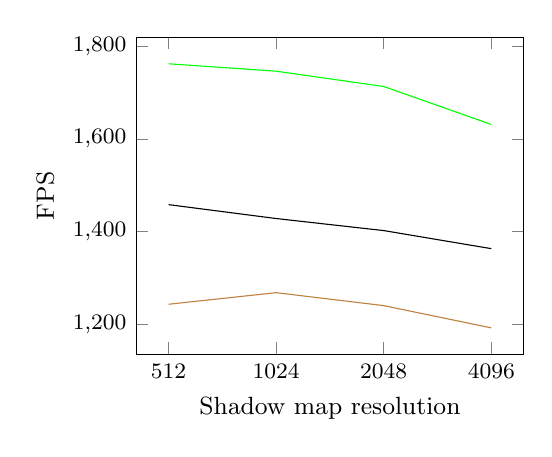
\begin{tikzpicture}
        \begin{semilogxaxis}[
            small,
            xlabel={Shadow map resolution},
            ylabel={FPS},
            xtick={512,1024,2048,4096},
            xticklabels={512,1024,2048,4096},
            % legend style={
            %     overlay,
            %     at={(1.25,0.5)},
            %     anchor=center},
            y tick label style={
                /pgf/number format/.cd,
                    fixed,   % po zakomentowaniu os rzednych jest indeksowana wykladniczo
                    fixed, % 1.0 zamiast 1
                    precision=1,
                /tikz/.cd
            },
            x tick label style={
                /pgf/number format/.cd,
                    fixed,
                    fixed,
                    precision=2,
                /tikz/.cd
            }
            ]
            \addplot [color=green]
            coordinates {
                (512,1762)(1024,1746)(2048,1713)(4096,1631)}; %\addlegendentry{720p}
            \addplot [color=black]
            coordinates {
                (512,1458)(1024,1428)(2048,1402)(4096,1363)}; %\addlegendentry{1080p}
            \addplot [color=brown]
            coordinates {
                (512,1243)(1024,1268)(2048,1240)(4096,1192)}; %\addlegendentry{2k}
        \end{semilogxaxis} 
    \end{tikzpicture}
    \caption{Results for the \textit{\textit{Chinese Dragon}} scene.}
    \label{fig:plot:basic_dragon}
\end{subfigure}
\hfill
\begin{subfigure}[t]{0.48\textwidth}
    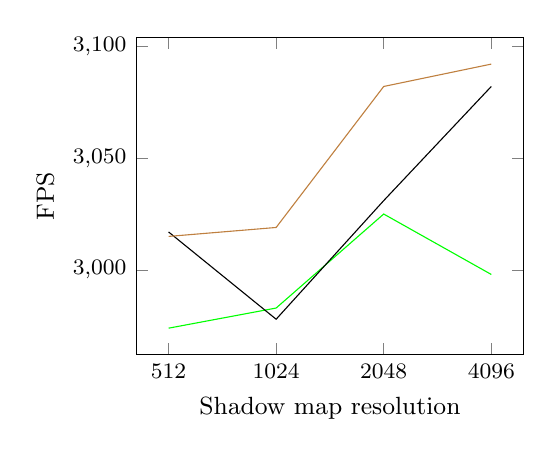
\begin{tikzpicture}
        \begin{semilogxaxis}[
            small,
            xlabel={Shadow map resolution},
            ylabel={FPS},
            xtick={512,1024,2048,4096},
            xticklabels={512,1024,2048,4096},
            % legend style={
            %     overlay,
            %     at={(1.25,0.5)},
            %     anchor=center},
            y tick label style={
                /pgf/number format/.cd,
                    fixed,   % po zakomentowaniu os rzednych jest indeksowana wykladniczo
                    fixed, % 1.0 zamiast 1
                    precision=1,
                /tikz/.cd
            },
            x tick label style={
                /pgf/number format/.cd,
                    fixed,
                    fixed,
                    precision=2,
                /tikz/.cd
            }
            ]
            \addplot [color=green]
            coordinates {
                (512,2974)(1024,2983)(2048,3025)(4096,2998)}; %\addlegendentry{720p}
            \addplot [color=black]
            coordinates {
                (512,3017)(1024,2978)(2048,3031)(4096,3082)}; %\addlegendentry{1080p}
            \addplot [color=brown]
            coordinates {
                (512,3015)(1024,3019)(2048,3082)(4096,3092)}; %\addlegendentry{2k}
        \end{semilogxaxis} 
    \end{tikzpicture}
    \caption{Results for the \textit{Cube} scene.}
    \label{fig:plot:basic_cube}
\end{subfigure}

\vspace{20pt}
\begin{subfigure}[t]{0.48\textwidth}
    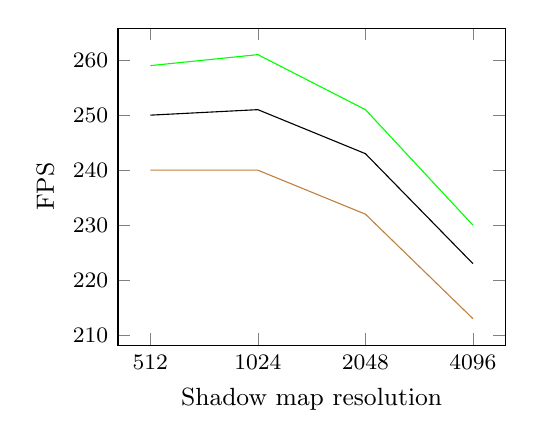
\begin{tikzpicture}
        \begin{semilogxaxis}[
            small,
            xlabel={Shadow map resolution},
            ylabel={FPS},
            xtick={512,1024,2048,4096},
            xticklabels={512,1024,2048,4096},
            % legend style={
            %     overlay,
            %     at={(1.25,0.5)},
            %     anchor=center},
            y tick label style={
                /pgf/number format/.cd,
                    fixed,   % po zakomentowaniu os rzednych jest indeksowana wykladniczo
                    fixed, % 1.0 zamiast 1
                    precision=1,
                /tikz/.cd
            },
            x tick label style={
                /pgf/number format/.cd,
                    fixed,
                    fixed,
                    precision=2,
                /tikz/.cd
            }
            ]
            \addplot [color=green]
            coordinates {
                (512,259)(1024,261)(2048,251)(4096,230)}; %\addlegendentry{720p}
            \addplot [color=black]
            coordinates {
                (512,250)(1024,251)(2048,243)(4096,223)}; %\addlegendentry{1080p}
            \addplot [color=brown]
            coordinates {
                (512,240)(1024,240)(2048,232)(4096,213)}; %\addlegendentry{2k}
        \end{semilogxaxis} 
    \end{tikzpicture}
    \caption{Results for the \textit{Power Plant} scene.}
    \label{fig:plot:basic_power}
\end{subfigure}
\hfill
\begin{subfigure}[t]{0.48\textwidth}
    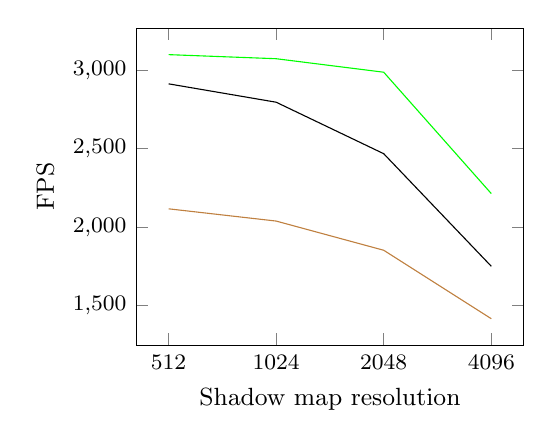
\begin{tikzpicture}
        \begin{semilogxaxis}[
            small,
            xlabel={Shadow map resolution},
            ylabel={FPS},
            xtick={512,1024,2048,4096},
            xticklabels={512,1024,2048,4096},
            % legend style={
            %     overlay,
            %     at={(1.25,0.5)},
            %     anchor=center},
            y tick label style={
                /pgf/number format/.cd,
                    fixed,   % po zakomentowaniu os rzednych jest indeksowana wykladniczo
                    fixed, % 1.0 zamiast 1
                    precision=1,
                /tikz/.cd
            },
            x tick label style={
                /pgf/number format/.cd,
                    fixed,
                    fixed,
                    precision=2,
                /tikz/.cd
            }
            ]
            \addplot [color=green]
            coordinates {
                (512,3098)(1024,3072)(2048,2986)(4096,2213)}; %\addlegendentry{720p}
            \addplot [color=black]
            coordinates {
                (512,2912)(1024,2795)(2048,2467)(4096,1750)}; %\addlegendentry{1080p}
            \addplot [color=brown]
            coordinates {
                (512,2116)(1024,2038)(2048,1852)(4096,1416)}; %\addlegendentry{2k}
        \end{semilogxaxis} 
    \end{tikzpicture}
    \caption{Results for the \textit{Crytek Sponza} scene.}
    \label{fig:plot:basic_sponza}
\end{subfigure}
\caption{Frames per second for all test scenes, for different sizes of the shadow map and output resolutions. In green \(1280\times 720\), in black \(1920\times 1080\) and in brown \(2560\times 1440\). Rendering with the basic shadow map implementation.}
\label{fig:plot:basic_results}
\end{figure}

The test results mostly match the expectation that fewer FPS will be produced with increasing shadow map resolution and output resolution. The only exception is plot \ref{fig:plot:basic_cube} of the \textit{Cube} scene results. This is however probably due to the fact that this scene is so simple, and in effect is rendered with such high FPS (highest in this test set, over 3000), that any interruptions from other programs on the machine will be visible. Inconsistencies might also be produced by hardware cores' dynamic clock rates, which can vary over the duration of the test.

The basic shadow mapping algorithm is simple enough to produce high FPS. Even in the most complex scene, the \textit{Power Plant}, over 210 frames are rendered at 2k output and 4k shadow map resolution.

Looking at the shapes of the plots, it can be said that the basic shadow mapping algorithm is not dependent on output resolution. The lower FPS for higher output resolutions stems mostly from the sole fact that more pixels need to be rendered, because the FPS falloffs along the x-axis follow the same shape for different output resolutions. In most cases the drop in FPS between the lowest and highest shadow map resolution is the same, regardless of the output resolution. 

The plots have their x-axis in logarithmic scale. Taking that into account, it can be observed that the FPS counts fall linearly with growing shadow map resolutions.

The algorithm's performance is not view-dependent. When traversing the scene the frame rates are stable. This is backed by the fact that in basic shadow mapping the same work is performed for each rendered pixel, consisting of a comparison operation with the depth value stored in the depth map. This however would not be true if shadow map fitting was used. In such case, the performance will become view dependent as more or less geometry will be rendered into the shadow map. This can provide a useful performance boost in large scenes.

Using the \textit{Tracy profiler} it can be confirmed that the renderer's performance is limited by the computations performed on the GPU, as the CPU thread spent approximately \(30\%\) of time waiting for the GPU resources to be available. \textit{Tracy} also reports that approximately \(40\%\) of the frame time was spent on the shadow map render pass and \(52\%\) on the main render pass. The remaining time was spent rendering the GUI and synchronizing. This can be expected as with this simple technique the shadow map pass is almost as expensive as the main pass. The main pass is slightly more involved as it outputs pixels and performs simple shading, as well as performs the shadow mapping itself, which requires texture lookups and comparisons that add time.

The rendering results for the \textit{Chinese Dragon} are presented in Fig. \ref{fig:test_basic_dragon_screens} and in Fig. \ref{fig:test_basic_sponza_screens} the \textit{Crytek Sponza} is presented.
\begin{figure}
    \centering
    \begin{subfigure}{0.48\textwidth}
		\centering
        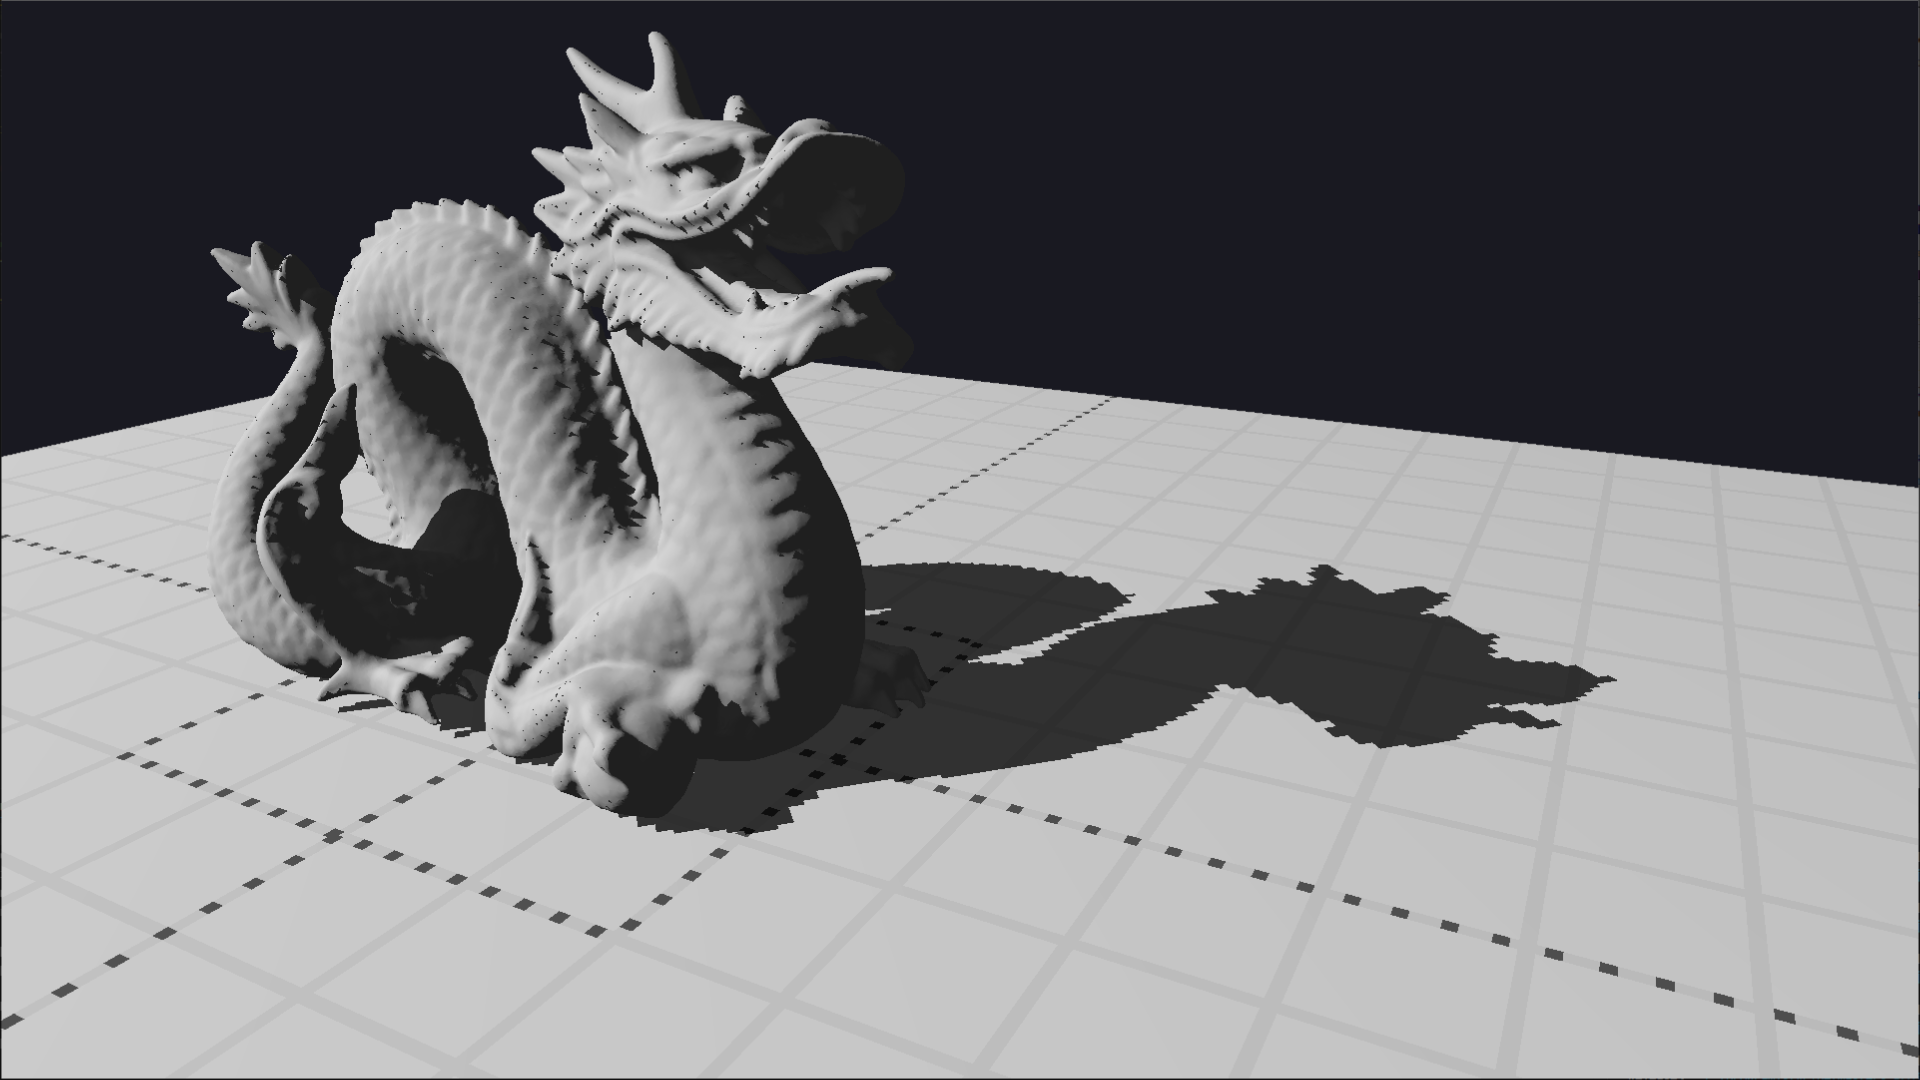
\includegraphics[width=\textwidth]{./graf/tests/basic/cropped/dragon_basic_fhd_512.png}
        \caption{The \textit{Chinese Dragon} rendered with \(512\times 512\) shadow map.}
    \end{subfigure}
	\hfill
    \begin{subfigure}{0.48\textwidth}
		\centering
        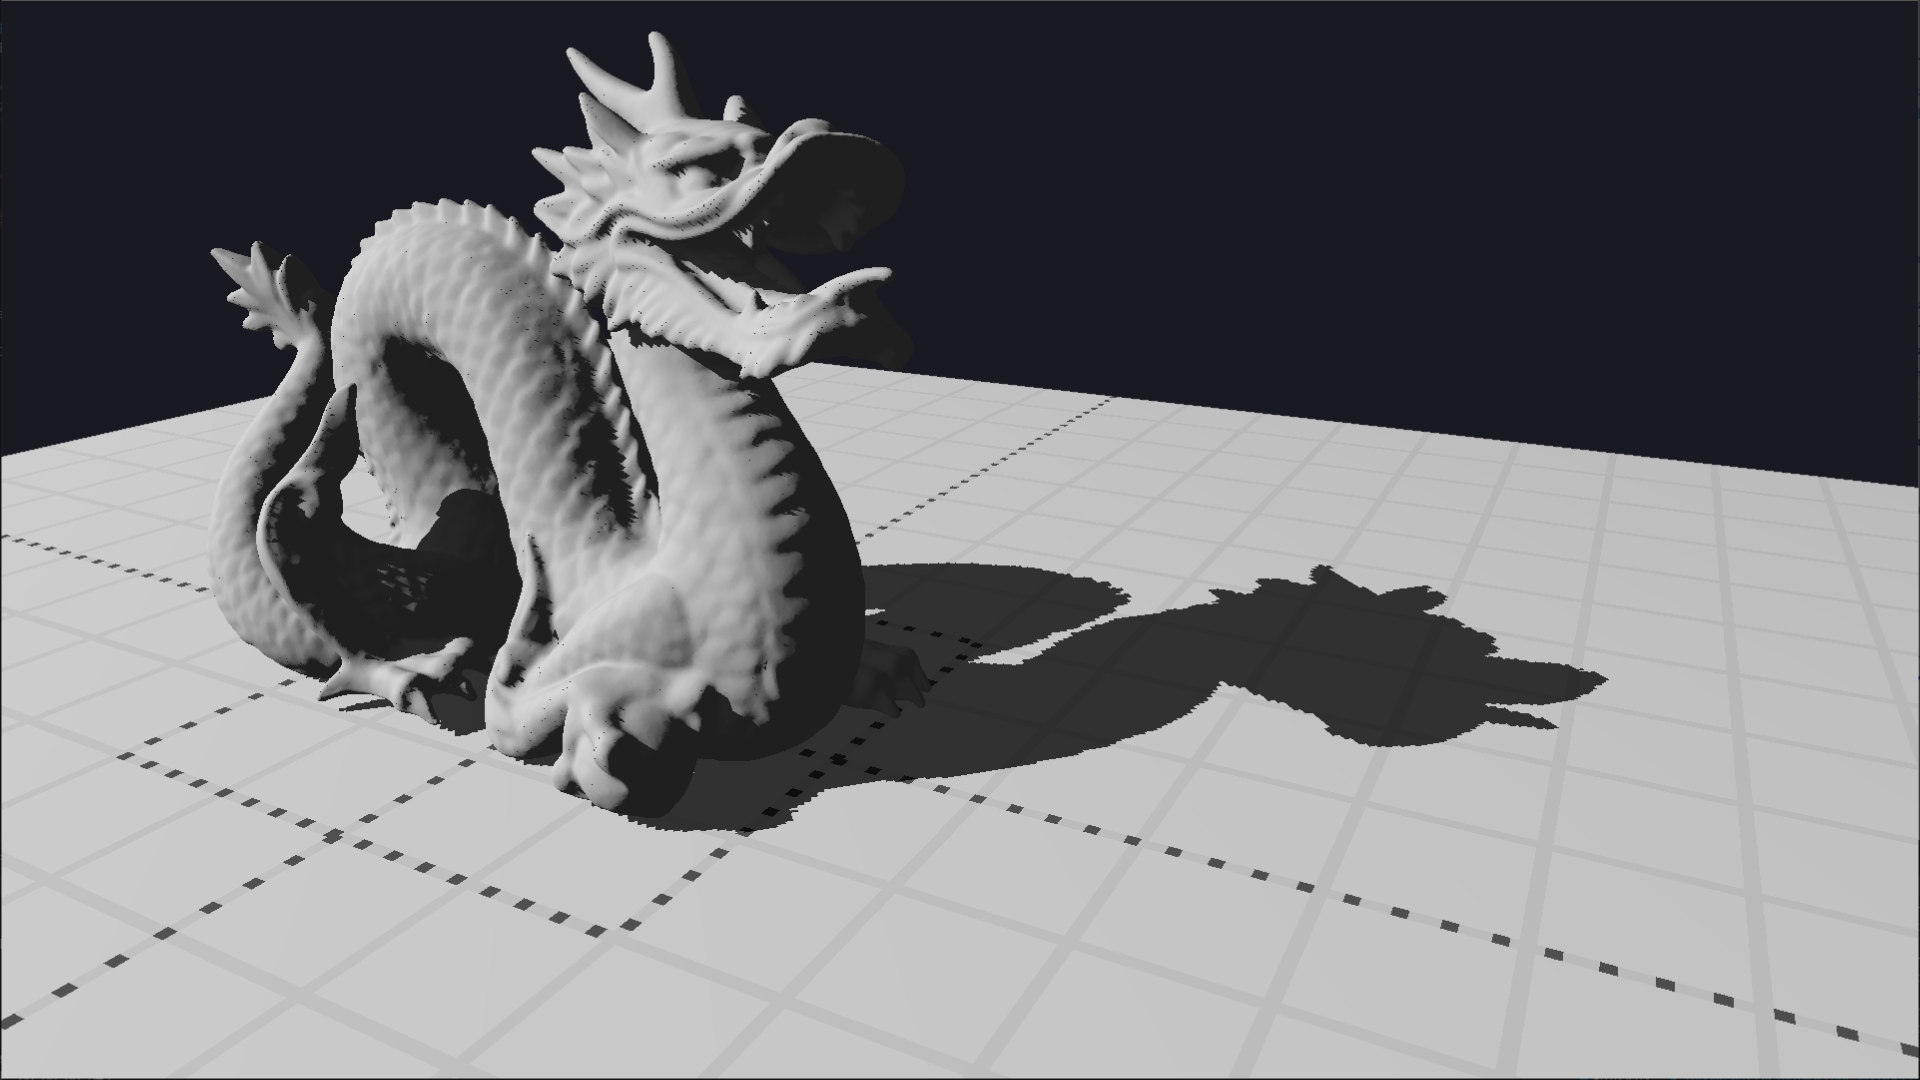
\includegraphics[width=\textwidth]{./graf/tests/basic/cropped/dragon_basic_fhd_1024.png}
        \caption{The \textit{Chinese Dragon} rendered with \(1024\times 1024\) shadow map.}
    \end{subfigure}

    \begin{subfigure}{0.48\textwidth}
		\centering
        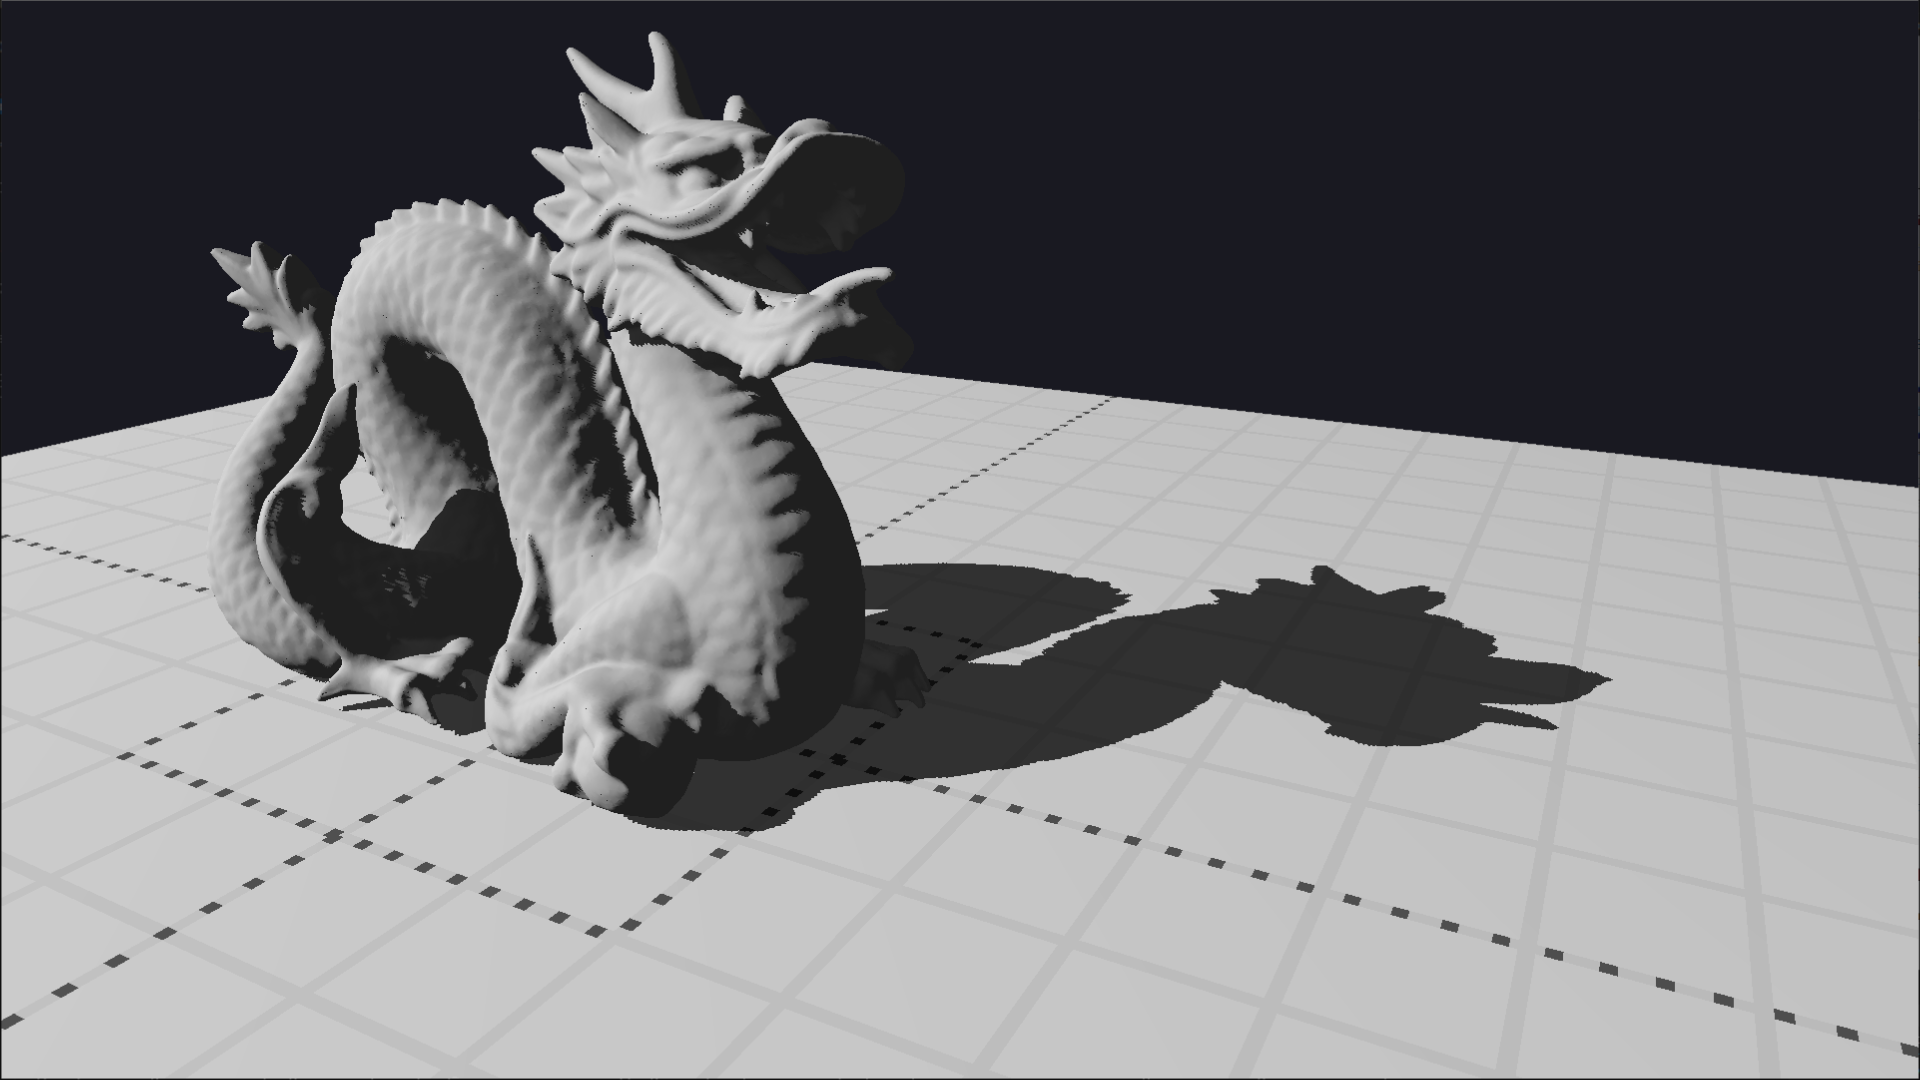
\includegraphics[width=\textwidth]{./graf/tests/basic/cropped/dragon_basic_fhd_2048.png}
        \caption{The \textit{Chinese Dragon} rendered with \(2048\times 2048\) shadow map.}
    \end{subfigure}
	\hfill
    \begin{subfigure}{0.48\textwidth}
		\centering
        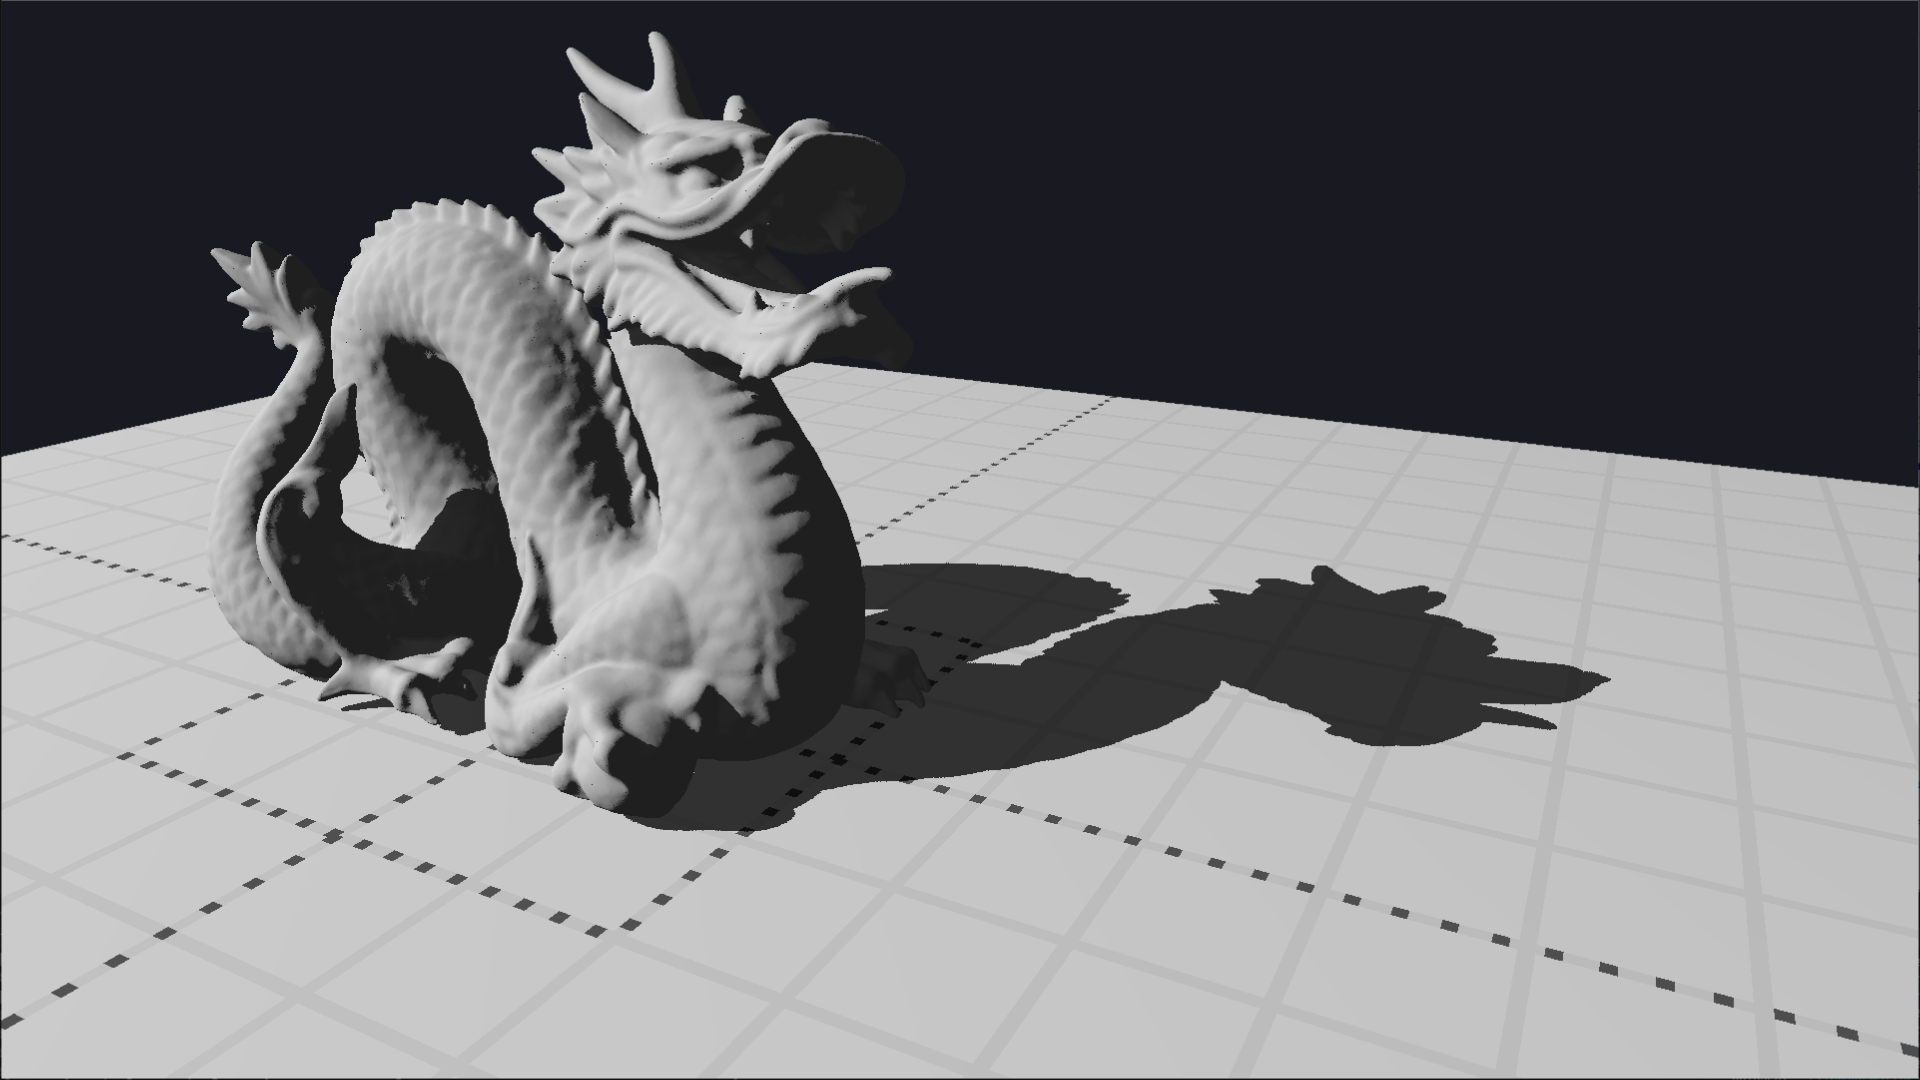
\includegraphics[width=\textwidth]{./graf/tests/basic/cropped/dragon_basic_fhd_4096.png}
        \caption{The \textit{Chinese Dragon} rendered with \(4096\times 4096\) shadow map.}
    \end{subfigure}

    \caption{The \textit{Chinese Dragon} scene rendered with different shadow map resolutions, using the basic shadow mapping algorithm.}
    \label{fig:test_basic_dragon_screens}
\end{figure}
\begin{figure}[t]
    \centering
    \begin{subfigure}{0.48\textwidth}
		\centering
        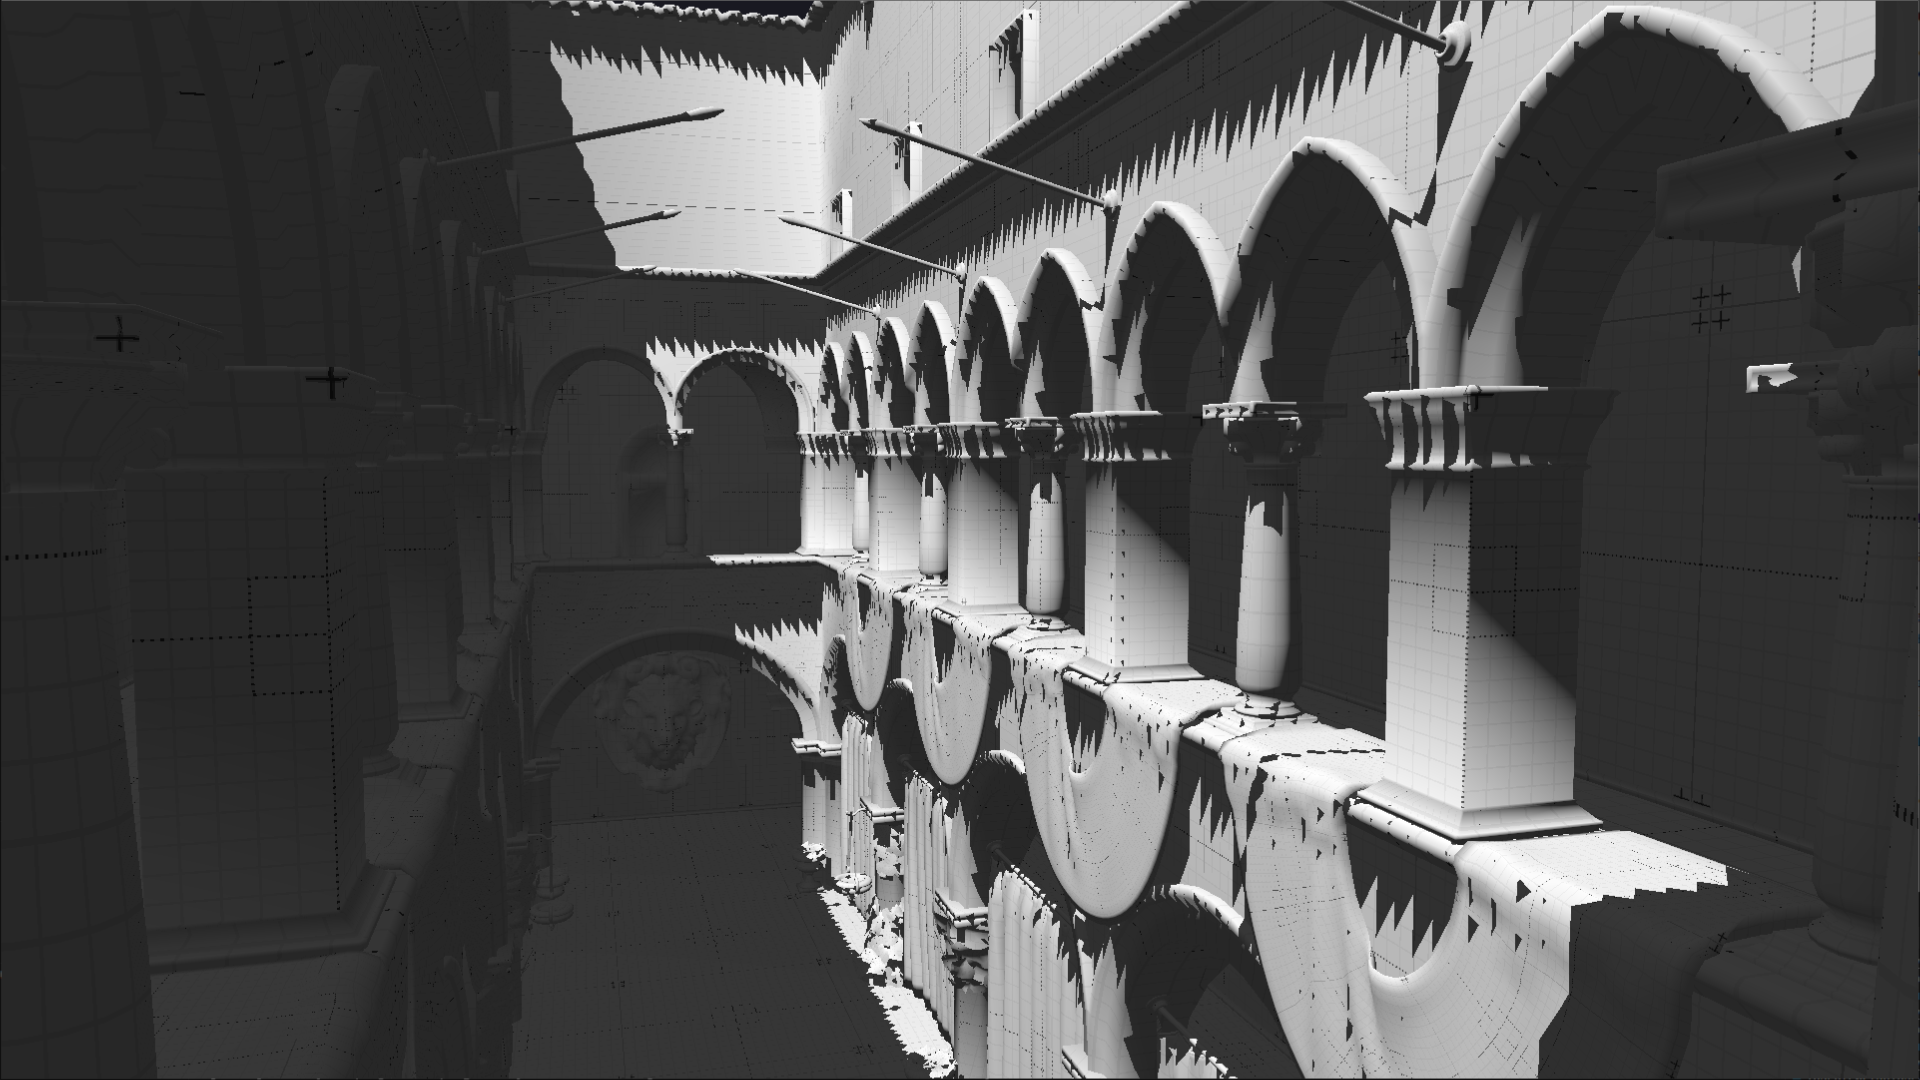
\includegraphics[width=\textwidth]{./graf/tests/basic/cropped/sponza_basic_fhd_512.png}
        \caption{The \textit{Crytek Sponza} rendered with \(512\times 512\) shadow map.}
    \end{subfigure}
	\hfill
    \begin{subfigure}{0.48\textwidth}
		\centering
        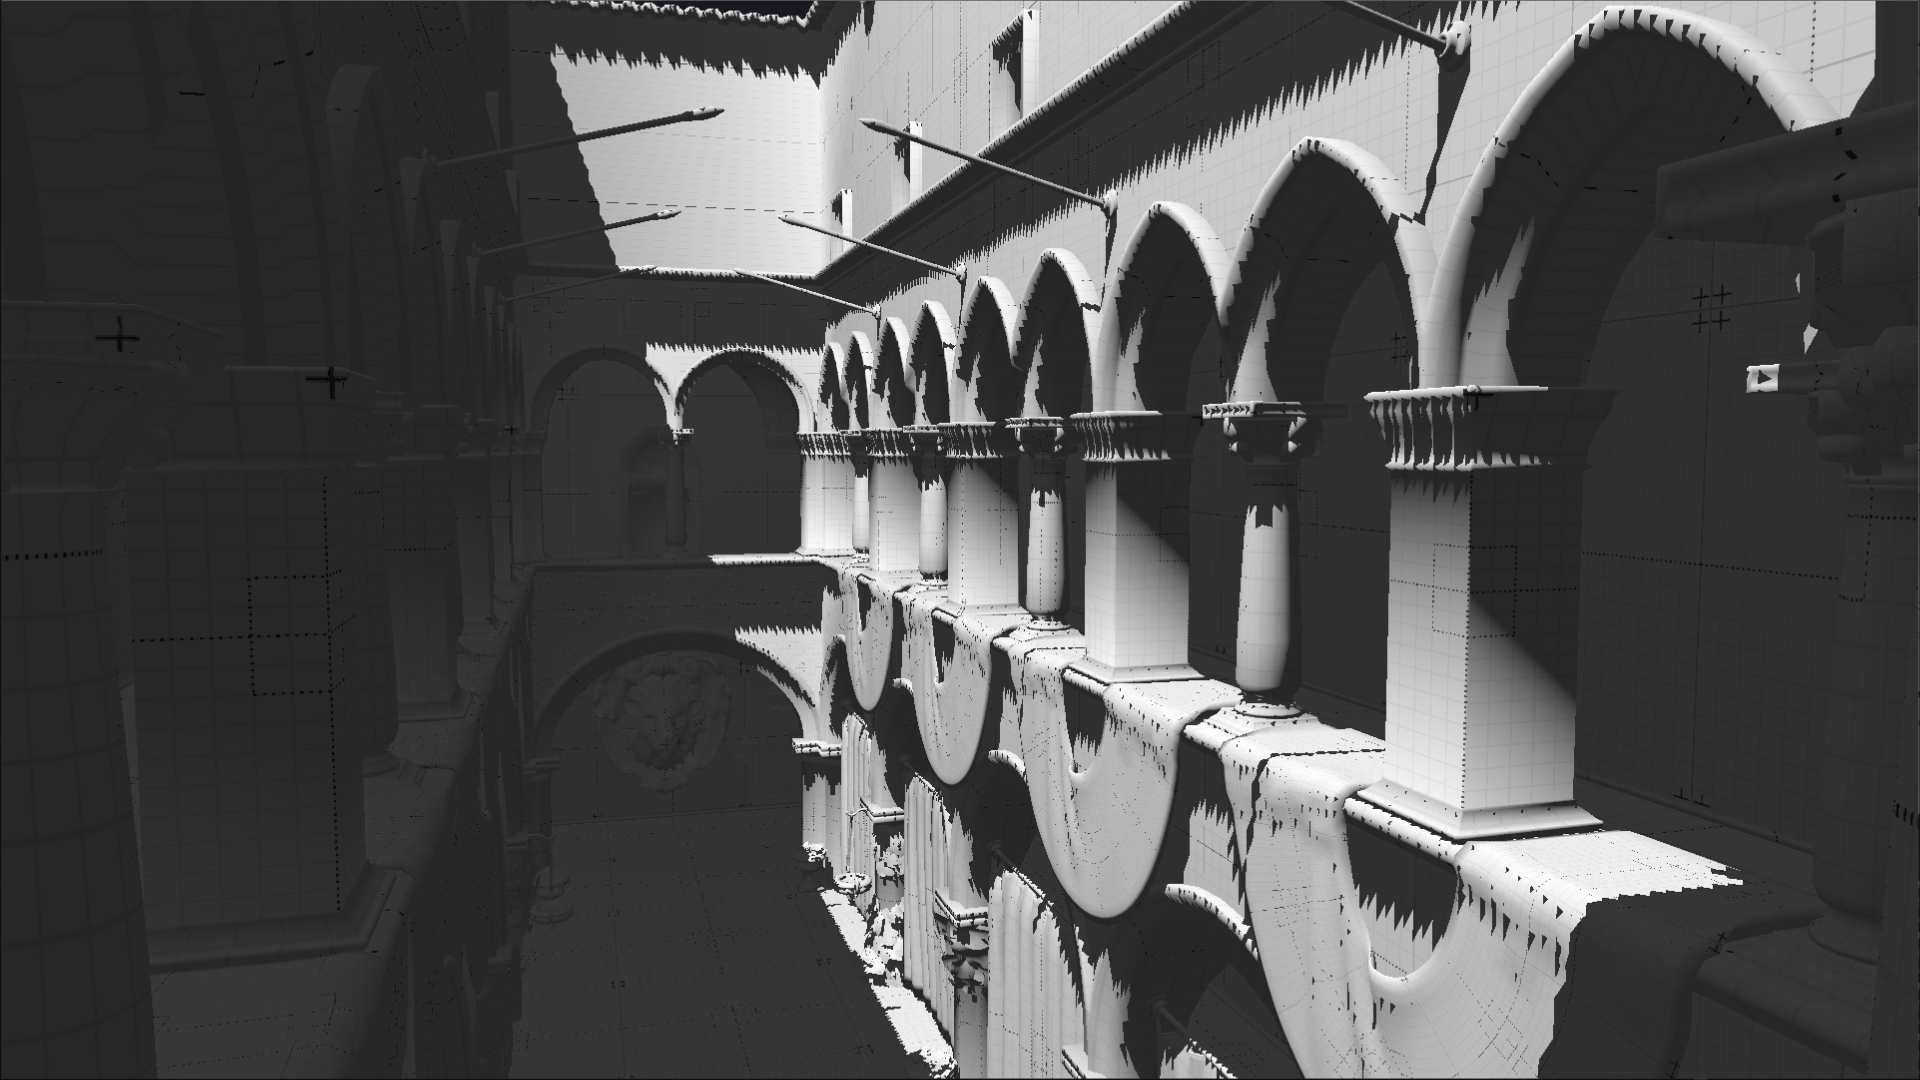
\includegraphics[width=\textwidth]{./graf/tests/basic/cropped/sponza_basic_fhd_1024.png}
        \caption{The \textit{\textit{Crytek Sponza}} rendered with \(1024\times 1024\) shadow map.}
    \end{subfigure}

    \begin{subfigure}{0.48\textwidth}
		\centering
        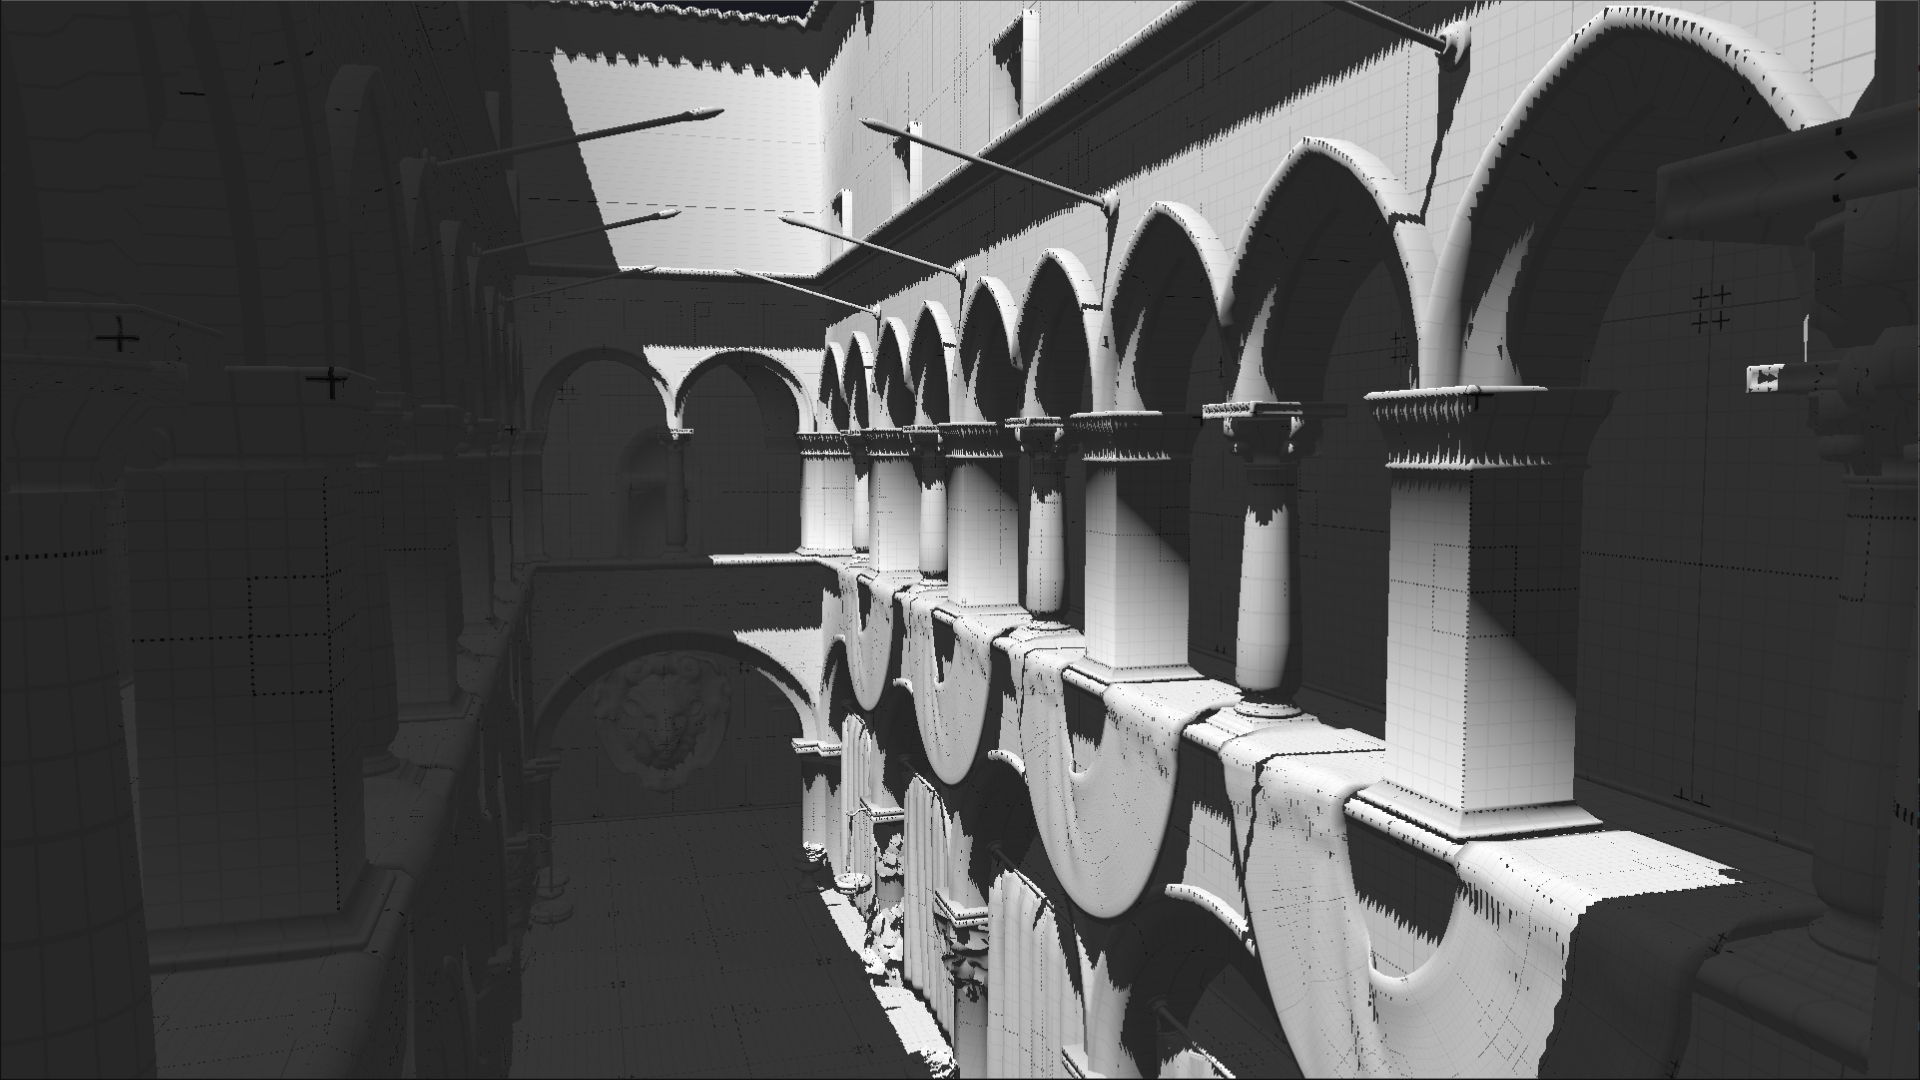
\includegraphics[width=\textwidth]{./graf/tests/basic/cropped/sponza_basic_fhd_2048.png}
        \caption{The \textit{Crytek Sponza} rendered with \(2048\times 2048\) shadow map.}
    \end{subfigure}
	\hfill
    \begin{subfigure}{0.48\textwidth}
		\centering
        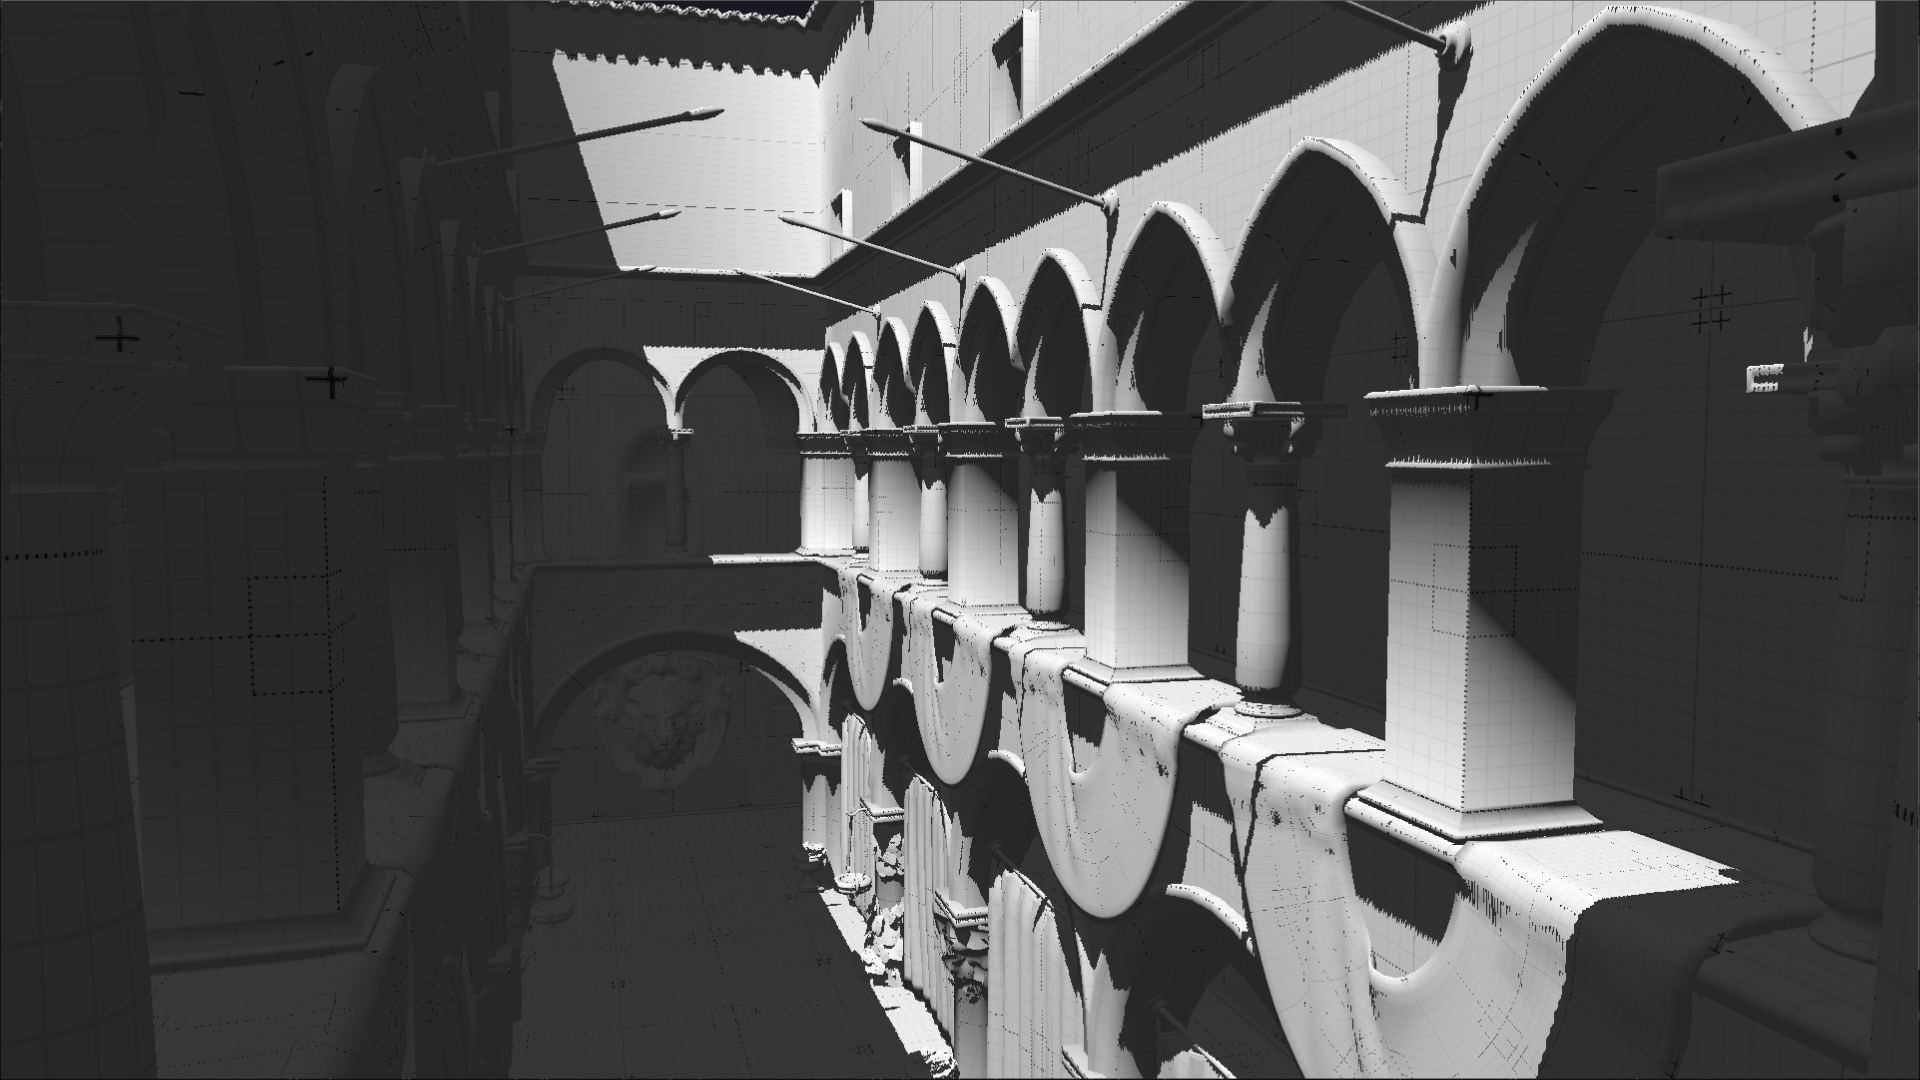
\includegraphics[width=\textwidth]{./graf/tests/basic/cropped/sponza_basic_fhd_4096.png}
        \caption{The \textit{Crytek Sponza} rendered with \(4096\times 4096\) shadow map.}
    \end{subfigure}

    \caption{The \textit{Crytek Sponza} scene rendered with different shadow map resolutions, using the basic shadow mapping algorithm.}
    \label{fig:test_basic_sponza_screens}
\end{figure}

The \textit{Chinese Dragon} results are quite good for higher resolution shadow maps, since the shadow map texels map many to one with regard to screen pixels. Aliasing is however very visible for lower resolutions. \textit{Crytek Sponza} suffers from shadow acne on vertical surfaces. This is a sign of badly chosen shadow bias. It gets less visible as resolution rises, but is always present. Even at the highest resolution, shadow map texel borders are still visible, where they were not visible in the \textit{Chinese Dragon} scene. This is due to the fact that the shadow map covers a larger area and each shadow map texel covers more space on the screen.

The memory usage is wholly dependent on the resolution of the shadow map. If memory is very scarce a depth buffer of lower precision can be used, but that is unlikely on modern graphics hardware to be the case. The depth map in this case was created to store the depth in 24 bits, plus additional 8 bits for the stencil buffer, totaling 32 bits per shadow map texel.

\subsection{Filtered shadow maps}
The following sections present experiments and their results performed using the implementations of different filtering techniques for shadow maps, which were described in sections \ref{section:filtering_shadow_maps} and \ref{section:pcf}.

\subsubsection{Hardware bilinear filtering}
\label{section:test_bilinear}
Hardware bilinear filtering is considered a simple filtering method that can improve appearance of shadows generated with shadow maps with practically no performance cost. This is tested for different output and shadow map resolutions in different test scenes and the results are presented in Fig. \ref{fig:plot:bilinear_results}.

\begin{figure}[h]
    \centering
    \begin{subfigure}[t]{0.48\textwidth}
        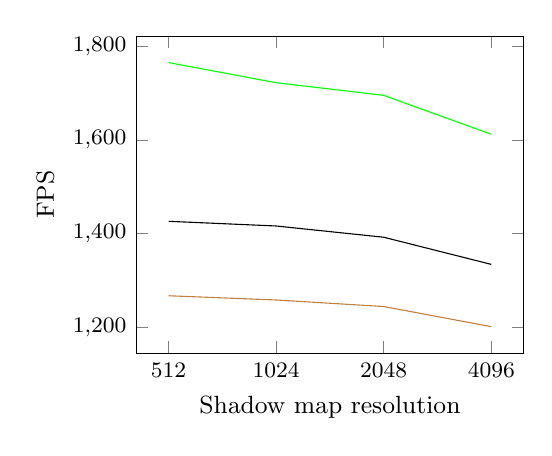
\begin{tikzpicture}
            \begin{semilogxaxis}[
                small,
                xlabel={Shadow map resolution},
                ylabel={FPS},
                xtick={512,1024,2048,4096},
                xticklabels={512,1024,2048,4096},
                % legend style={
                %     overlay,
                %     at={(1.25,0.5)},
                %     anchor=center},
                y tick label style={
                    /pgf/number format/.cd,
                        fixed,   % po zakomentowaniu os rzednych jest indeksowana wykladniczo
                        fixed, % 1.0 zamiast 1
                        precision=1,
                    /tikz/.cd
                },
                x tick label style={
                    /pgf/number format/.cd,
                        fixed,
                        fixed,
                        precision=2,
                    /tikz/.cd
                }
                ]
                \addplot [color=green]
                coordinates {
                    (512,1765)(1024,1722)(2048,1695)(4096,1612)}; %\addlegendentry{720p}
                \addplot [color=black]
                coordinates {
                    (512,1426)(1024,1416)(2048,1392)(4096,1334)}; %\addlegendentry{1080p}
                \addplot [color=brown]
                coordinates {
                    (512,1267)(1024,1258)(2048,1244)(4096,1201)}; %\addlegendentry{2k}
            \end{semilogxaxis} 
        \end{tikzpicture}
        \caption{Results for the \textit{Chinese Dragon} scene.}
        \label{fig:plot:bilinear_dragon}
    \end{subfigure}
    \hfill
    \begin{subfigure}[t]{0.48\textwidth}
        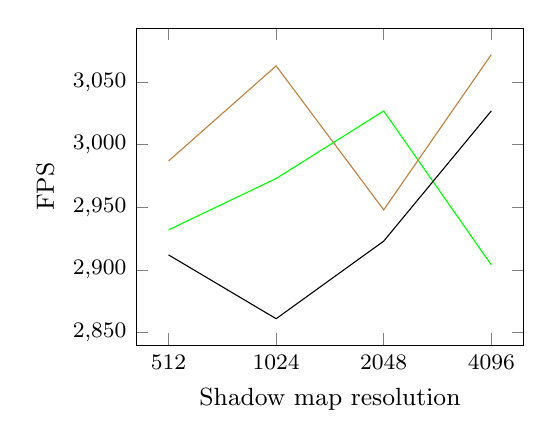
\begin{tikzpicture}
            \begin{semilogxaxis}[
                small,
                xlabel={Shadow map resolution},
                ylabel={FPS},
                xtick={512,1024,2048,4096},
                xticklabels={512,1024,2048,4096},
                % legend style={
                %     overlay,
                %     at={(1.25,0.5)},
                %     anchor=center},
                y tick label style={
                    /pgf/number format/.cd,
                        fixed,   % po zakomentowaniu os rzednych jest indeksowana wykladniczo
                        fixed, % 1.0 zamiast 1
                        precision=1,
                    /tikz/.cd
                },
                x tick label style={
                    /pgf/number format/.cd,
                        fixed,
                        fixed,
                        precision=2,
                    /tikz/.cd
                }
                ]
                \addplot [color=green]
                coordinates {
                    (512,2932)(1024,2973)(2048,3027)(4096,2904)}; %\addlegendentry{720p}
                \addplot [color=black]
                coordinates {
                    (512,2912)(1024,2861)(2048,2923)(4096,3027)}; %\addlegendentry{1080p}
                \addplot [color=brown]
                coordinates {
                    (512,2987)(1024,3063)(2048,2948)(4096,3072)}; %\addlegendentry{2k}
            \end{semilogxaxis} 
        \end{tikzpicture}
        \caption{Results for the \textit{Cube} scene.}
        \label{fig:plot:bilinear_cube}
    \end{subfigure}
    
    \vspace{20pt}
    \begin{subfigure}[t]{0.48\textwidth}
        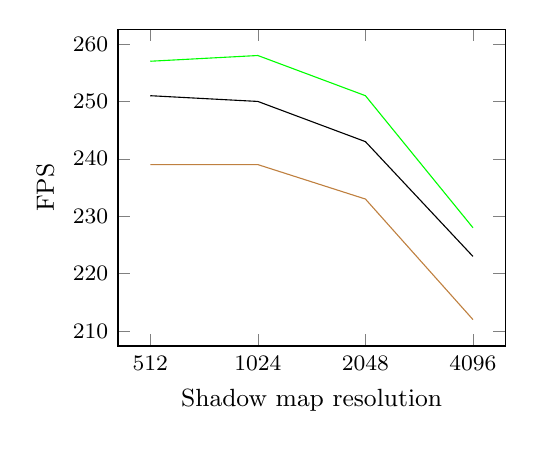
\begin{tikzpicture}
            \begin{semilogxaxis}[
                small,
                xlabel={Shadow map resolution},
                ylabel={FPS},
                xtick={512,1024,2048,4096},
                xticklabels={512,1024,2048,4096},
                % legend style={
                %     overlay,
                %     at={(1.25,0.5)},
                %     anchor=center},
                y tick label style={
                    /pgf/number format/.cd,
                        fixed,   % po zakomentowaniu os rzednych jest indeksowana wykladniczo
                        fixed, % 1.0 zamiast 1
                        precision=1,
                    /tikz/.cd
                },
                x tick label style={
                    /pgf/number format/.cd,
                        fixed,
                        fixed,
                        precision=2,
                    /tikz/.cd
                }
                ]
                \addplot [color=green]
                coordinates {
                    (512,257)(1024,258)(2048,251)(4096,228)}; %\addlegendentry{720p}
                \addplot [color=black]
                coordinates {
                    (512,251)(1024,250)(2048,243)(4096,223)}; %\addlegendentry{1080p}
                \addplot [color=brown]
                coordinates {
                    (512,239)(1024,239)(2048,233)(4096,212)}; %\addlegendentry{2k}
            \end{semilogxaxis} 
        \end{tikzpicture}
        \caption{Results for the \textit{\textit{Power Plant}} scene.}
        \label{fig:plot:bilinear_power}
    \end{subfigure}
    \hfill
    \begin{subfigure}[t]{0.48\textwidth}
        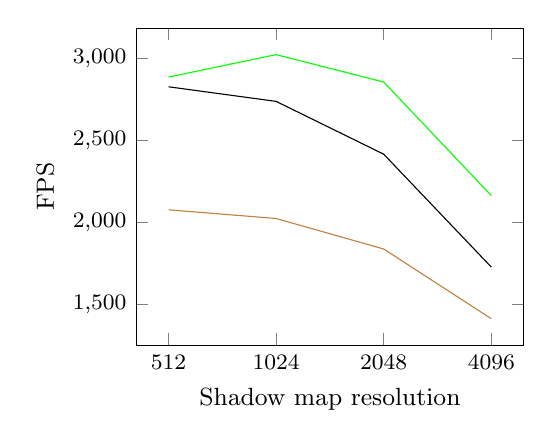
\begin{tikzpicture}
            \begin{semilogxaxis}[
                small,
                xlabel={Shadow map resolution},
                ylabel={FPS},
                xtick={512,1024,2048,4096},
                xticklabels={512,1024,2048,4096},
                % legend style={
                %     overlay,
                %     at={(1.25,0.5)},
                %     anchor=center},
                y tick label style={
                    /pgf/number format/.cd,
                        fixed,   % po zakomentowaniu os rzednych jest indeksowana wykladniczo
                        fixed, % 1.0 zamiast 1
                        precision=1,
                    /tikz/.cd
                },
                x tick label style={
                    /pgf/number format/.cd,
                        fixed,
                        fixed,
                        precision=2,
                    /tikz/.cd
                }
                ]
                \addplot [color=green]
                coordinates {
                    (512,2884)(1024,3021)(2048,2854)(4096,2162)}; %\addlegendentry{720p} here at 4k drpos <10 fps visible
                \addplot [color=black]
                coordinates {
                    (512,2825)(1024,2736)(2048,2414)(4096,1726)}; %at 4k shadow map, visible difference of few fps, sometimes... %\addlegendentry{1080p}
                \addplot [color=brown]
                coordinates {
                    (512,2075)(1024,2022)(2048,1836)(4096,1411)}; %\addlegendentry{2k}
            \end{semilogxaxis} 
        \end{tikzpicture}
        \caption{Results for the \textit{Crytek Sponza} scene.}
        \label{fig:plot:bilinear_sponza}
    \end{subfigure}
    \caption{Frames per second for all test scenes, for different sizes of the shadow map and output resolutions. In green \(1280\times 720\), in black \(1920\times 1080\) and in brown \(2560\times 1440\). Rendering with the basic shadow mapping technique with bilinear filtering enabled.}
    \label{fig:plot:bilinear_results}
\end{figure}

The results are very similar, with no immediately visible drop in performance. Taking the \textit{\textit{Power Plant}} scene as an example, the FPS range measured at Full HD output resolution is \([251:223]\). In the shadow mapping without filtering test the FPS range was \([250:223]\). The results are the same when accounting for instabilities caused by other software and dynamic clock rates. This is interesting when compared to results of \textit{Crytek Sponza} tests, where the Full HD range was \([2825:1726]\) with bilinear filtering and  \([2912:1750]\) without. Here, a significant drop in performance can be seen when using bilinear filtering. This might be caused by the fact FPS measurements are more sensitive in higher rages, as 1 FPS difference at 250 FPS is equal to 0.016ms, while 1 FPS difference at 2800 FPS is equal to only 0,000127ms. This is somewhat visible in the \textit{Crytek Sponza} FPS ranges, as the upper ends have a higher difference between them than lower ends. Additionally, since the \textit{Power Plant} is a much heavier scene performance-wise, the GPU has much more work to perform and the slowdown from using bilinear filtering can get masked better. When toggling bilinear filtering on and off during testing, the FPS readout would most of the time stay stable within reasonable FPS ranges. It seems that the cost of hardware bilinear filtering is indeed insignificant in realistic scenarios, where the GPU is fully utilized.

The effect on the final rendered result is on the other hand very significant, especially at lower shadow map resolutions, as presented in figure \ref{fig:test_bilinear_dragon_screens}. The shadow boundaries get smoother, which improves the visuals even at low shadow map resolutions. The texels are less noticeable and the shape is more easily readable as a shadow.

\begin{figure}[h]
    \centering
    \begin{subfigure}[t]{0.48\textwidth}
		\centering
        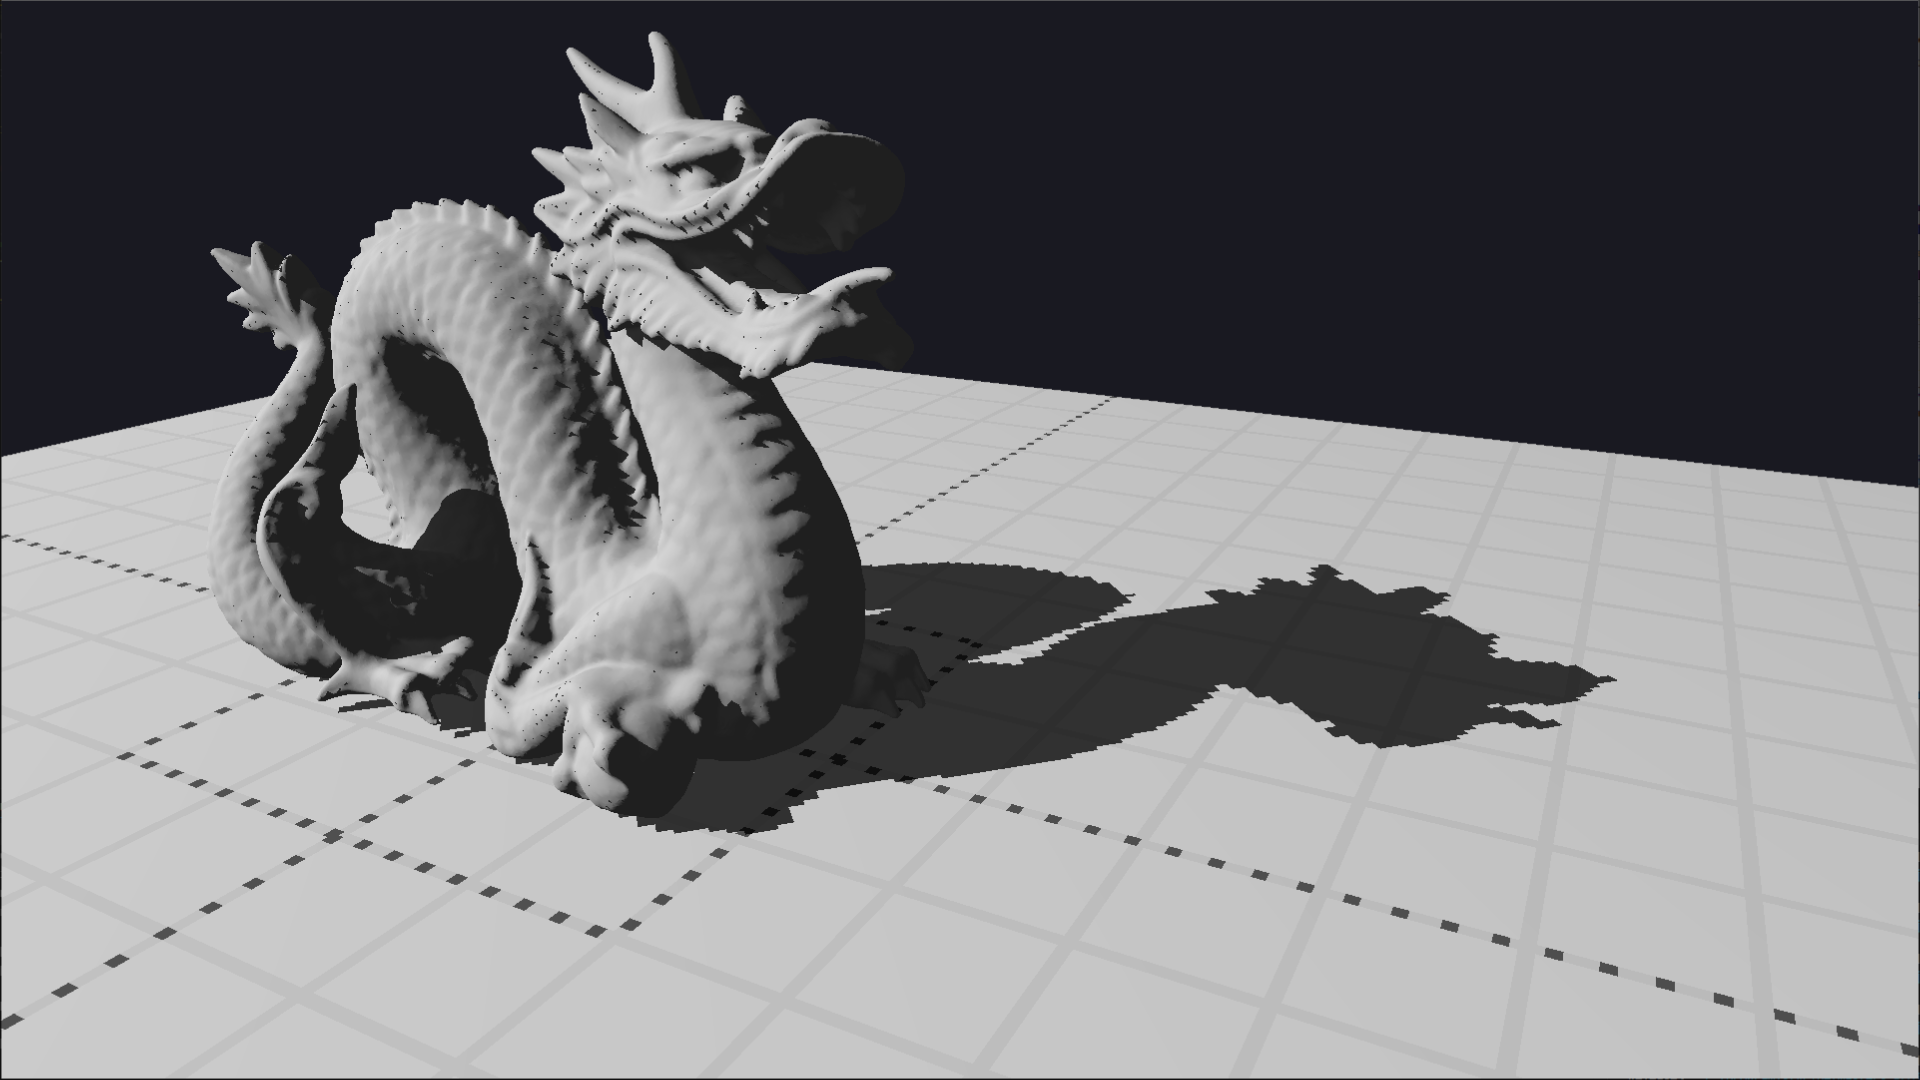
\includegraphics[width=\textwidth]{./graf/tests/basic/cropped/dragon_basic_fhd_512.png}
        \caption{The \textit{Chinese Dragon} rendered with a \(512\times 512\) shadow map with no filtering.}
    \end{subfigure}
	\hfill
    \begin{subfigure}[t]{0.48\textwidth}
		\centering
        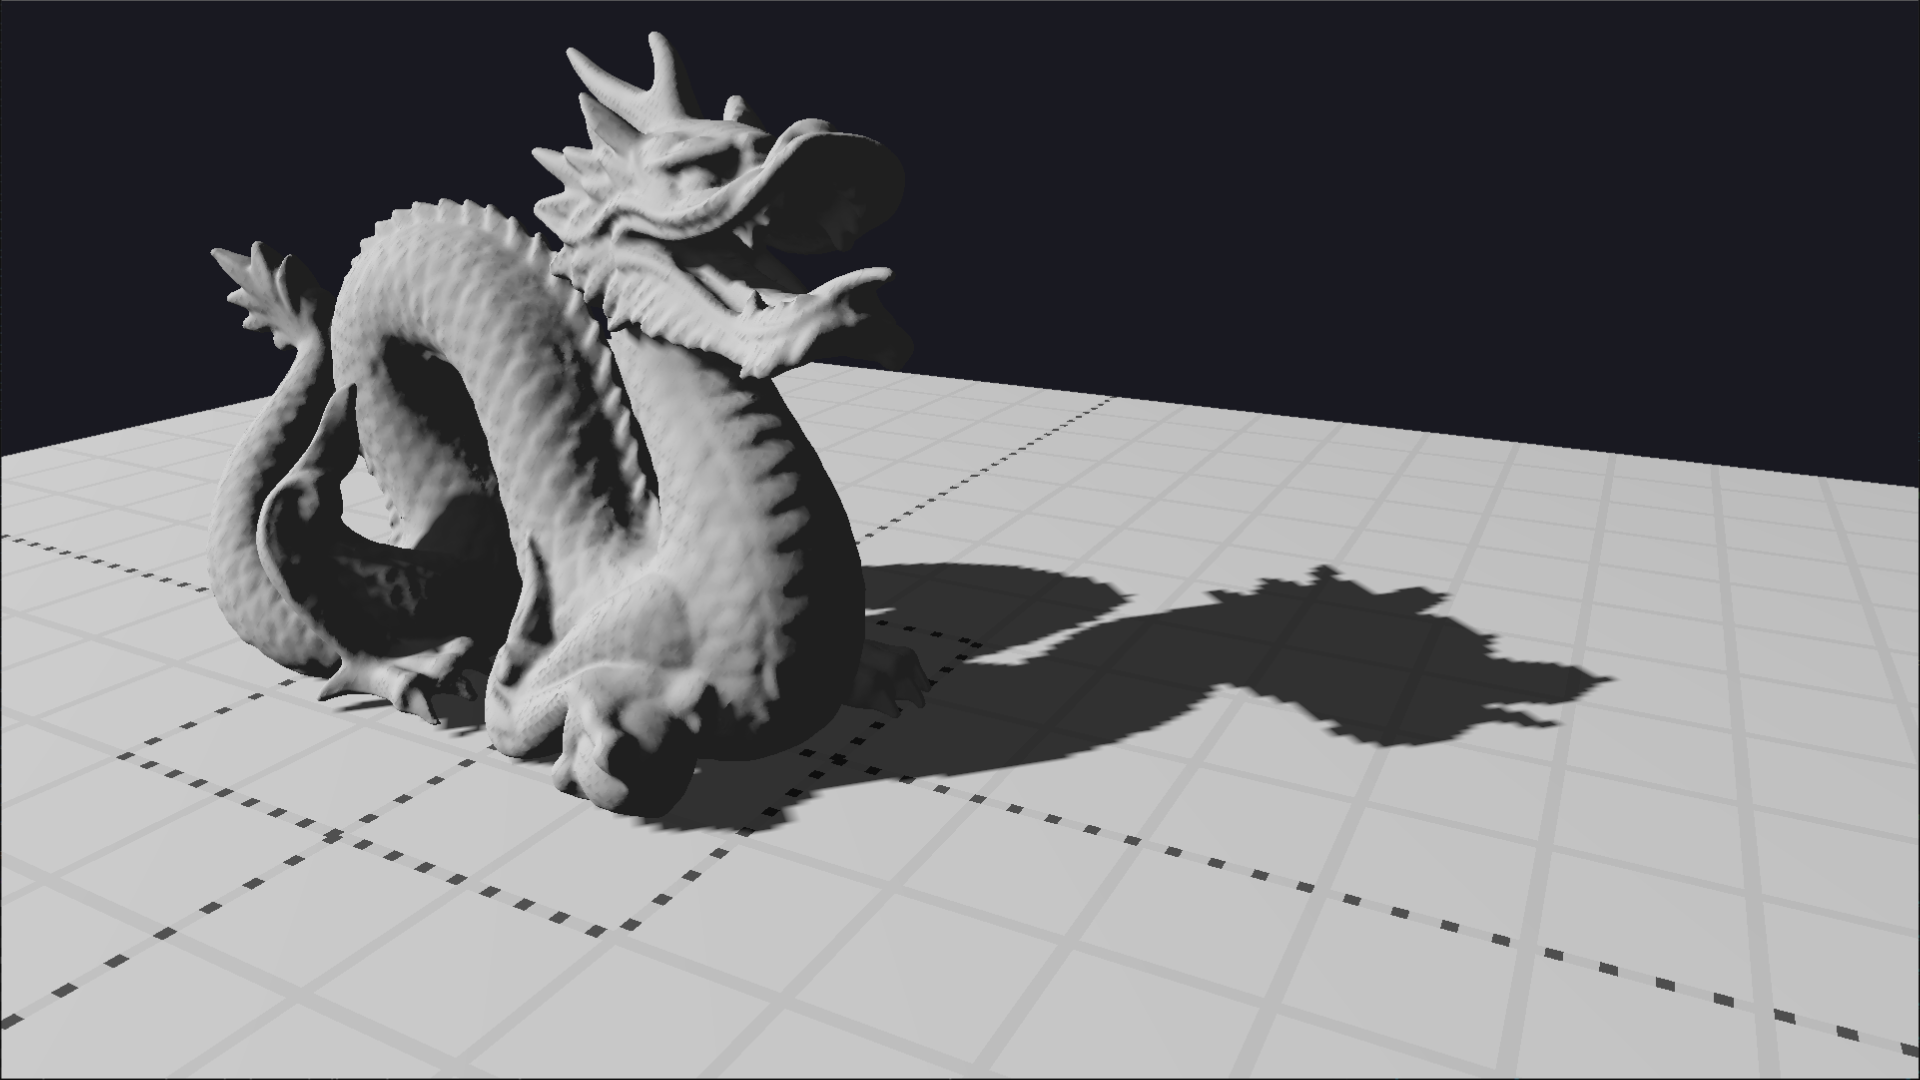
\includegraphics[width=\textwidth]{./graf/tests/bilinear/cropped/dragon_bilinear_fhd_512.png}
        \caption{The \textit{Chinese Dragon} rendered with a \(512\times 512\) shadow map with bilinear filtering.}
    \end{subfigure}
    \begin{subfigure}[t]{0.48\textwidth}
		\centering
        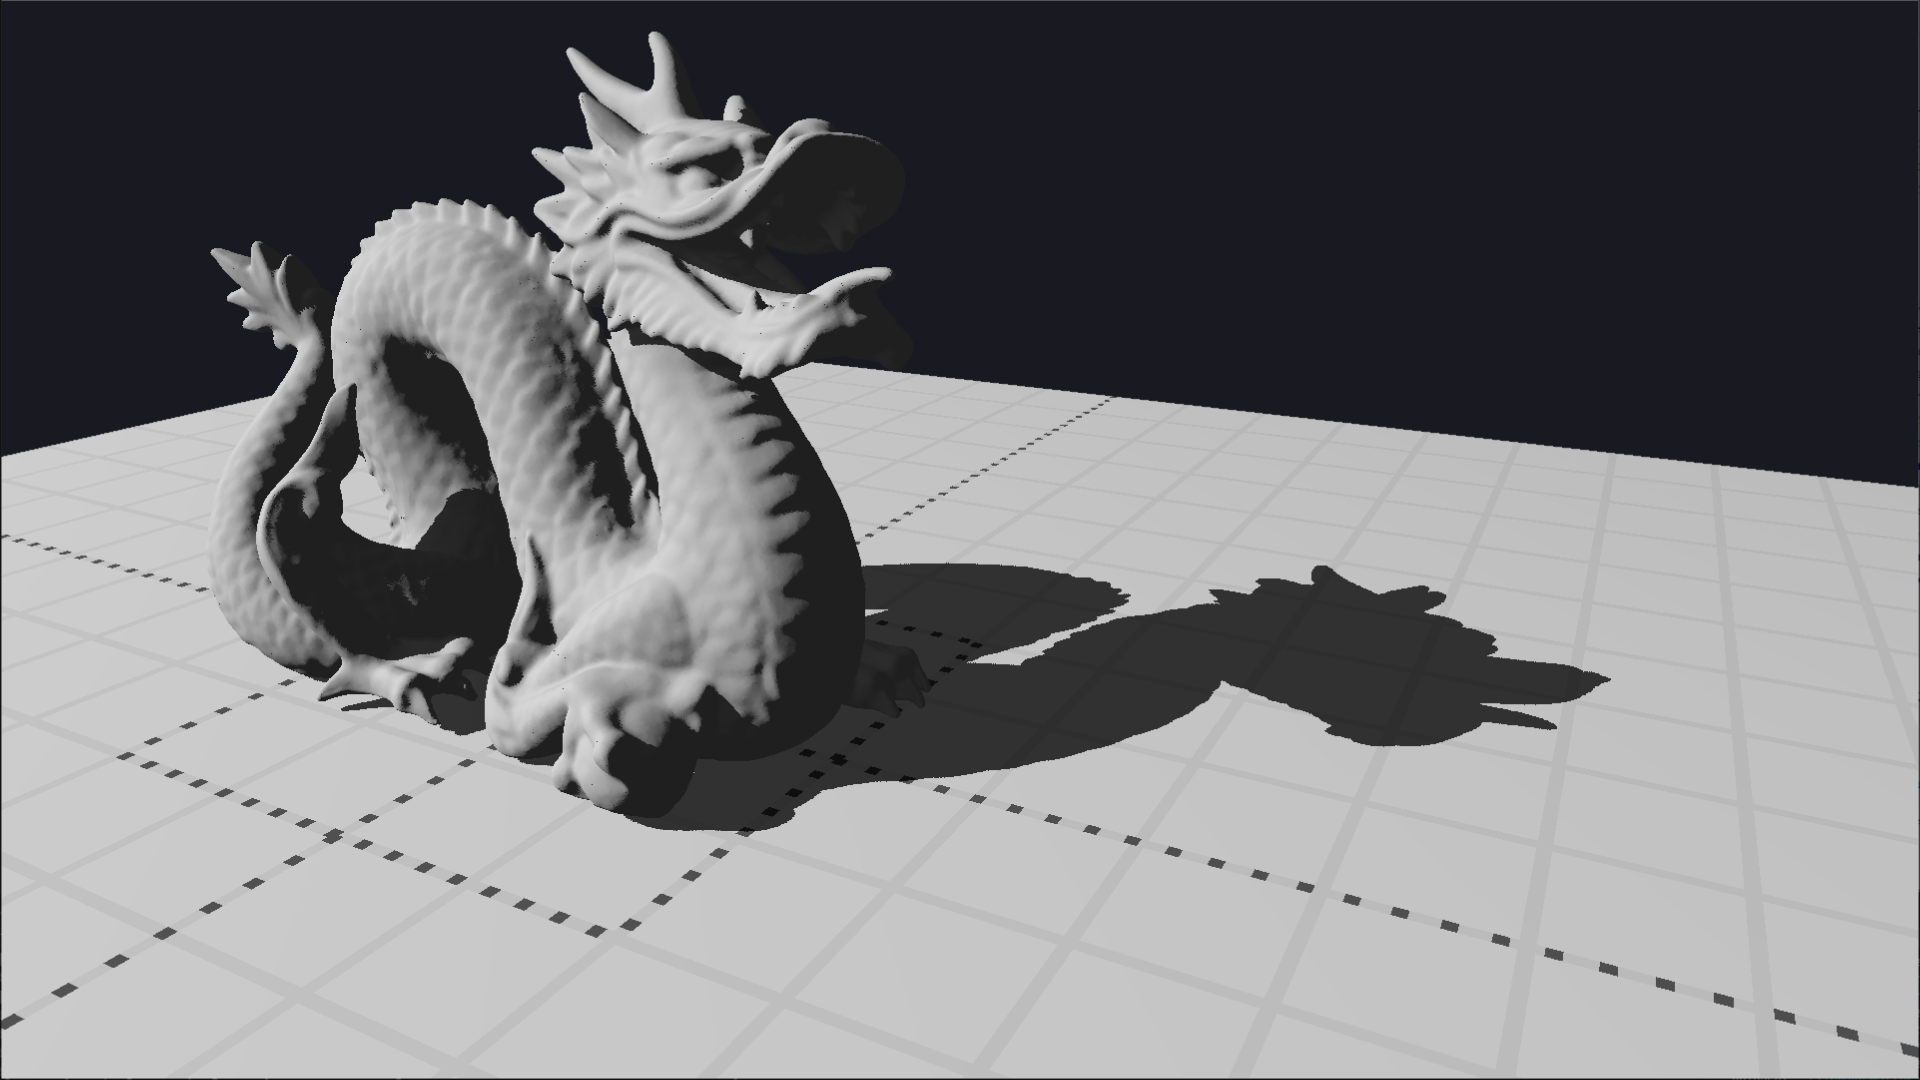
\includegraphics[width=\textwidth]{./graf/tests/basic/cropped/dragon_basic_fhd_4096.png}
        \caption{The \textit{Chinese Dragon} rendered with a \(4096\times 4096\) shadow map with no filtering.}
    \end{subfigure}
	\hfill
    \begin{subfigure}[t]{0.48\textwidth}
		\centering
        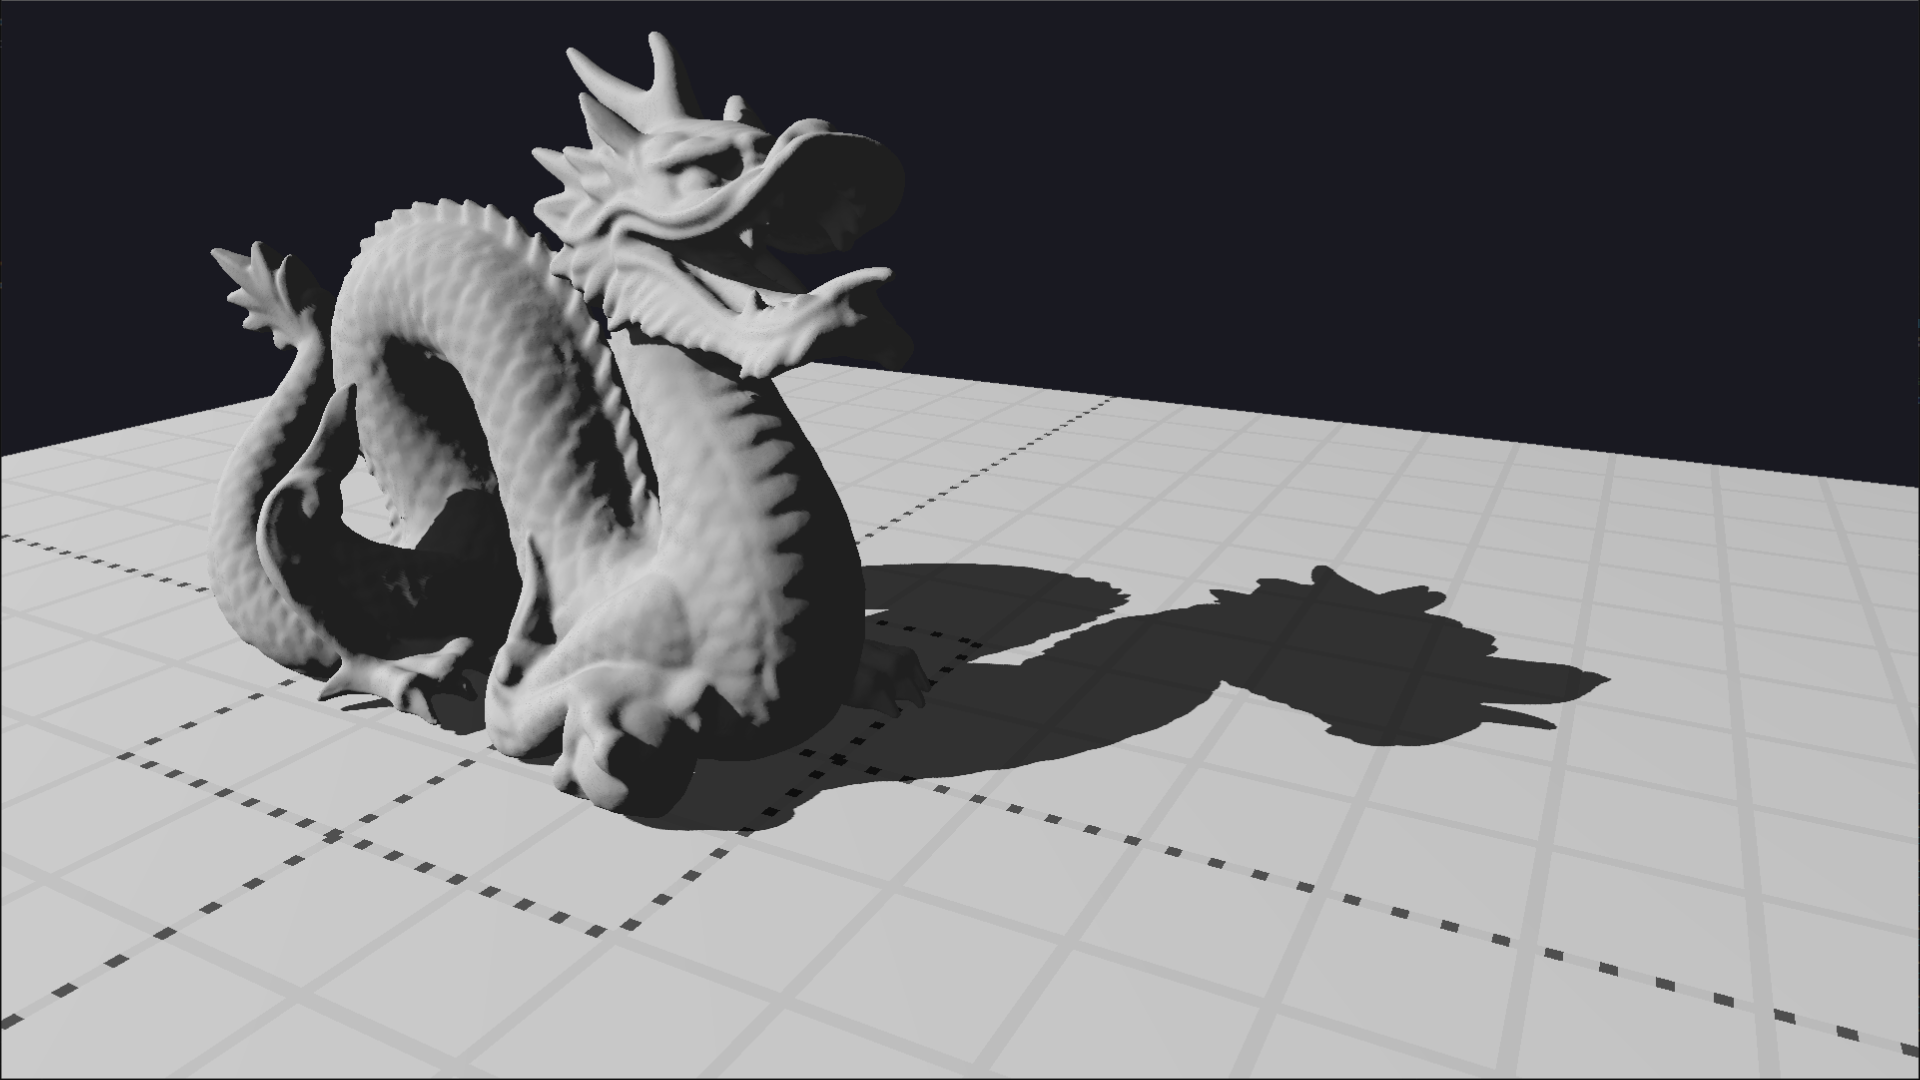
\includegraphics[width=\textwidth]{./graf/tests/bilinear/cropped/dragon_bilinear_fhd_4096.png}
        \caption{The \textit{Chinese Dragon} rendered with a \(4096\times 4096\) shadow map with bilinear filtering.}
    \end{subfigure}

    \caption{The \textit{Chinese Dragon} rendered with and without bilinear comparison filtering.}
    \label{fig:test_bilinear_dragon_screens}
\end{figure}

Unfortunately, this filtering means that biasing has to be adjusted, as samples will be taken around the original position. This results in visible shadow acne, especially at lower shadow map resolutions, where shadow map texels cover a larger area on screen. It's noteworthy that, while there will be more pixels that erroneously self-shadow, the contrast of such artifacts will be smaller. This can help hide them at higher shadow map resolutions.

\subsubsection{Percentage-closer filtering}
PCF is another filtering technique that allows for the creation of arbitrarily sized filter kernels used to filter the results of shadow computations. For the performance tests, the shadow map resolution will be kept constant to measure how kernel size and output resolution affect the FPS counts. Shadow map resolution does not impact the results in the context of this technique, apart from the performance degradation with higher shadow map resolutions observed in previous tests. The results for all scenes, for different square filter kernel sizes and output resolutions are presented in Fig. \ref{fig:plot:pcf_results}.
\begin{figure}[h]
    \centering
    \begin{subfigure}[t]{0.48\textwidth}
        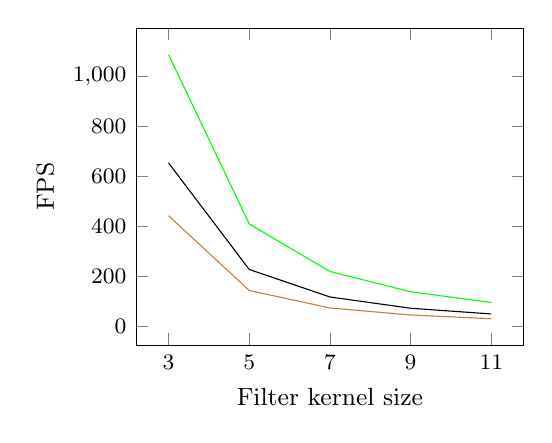
\begin{tikzpicture}
            \begin{axis}[
                small,
                xlabel={Filter kernel size},
                ylabel={FPS},
                xtick={3,5,7,9,11},
                xticklabels={3,5,7,9,11},
                % legend style={
                %     overlay,
                %     at={(1.25,0.5)},
                %     anchor=center},
                y tick label style={
                    /pgf/number format/.cd,
                        fixed,   % po zakomentowaniu os rzednych jest indeksowana wykladniczo
                        fixed, % 1.0 zamiast 1
                        precision=1,
                    /tikz/.cd
                },
                x tick label style={
                    /pgf/number format/.cd,
                        fixed,
                        fixed,
                        precision=2,
                    /tikz/.cd
                }
                ]
                \addplot [color=green]
                coordinates {
                    (3,1087)(5,410)(7,220)(9,139)(11,96)}; %\addlegendentry{720p}
                \addplot [color=black]
                coordinates {
                    (3,654)(5,228)(7,118)(9,73)(11,50)}; %\addlegendentry{1080p}
                \addplot [color=brown]
                coordinates {
                    (3,443)(5,144)(7,74)(9,46)(11,31)}; %\addlegendentry{2k}
            \end{axis} 
        \end{tikzpicture}
        \caption{Results for the \textit{Chinese Dragon} scene.}
        \label{fig:plot:pcf_dragon}
    \end{subfigure}
    \hfill
    \begin{subfigure}[t]{0.48\textwidth}
        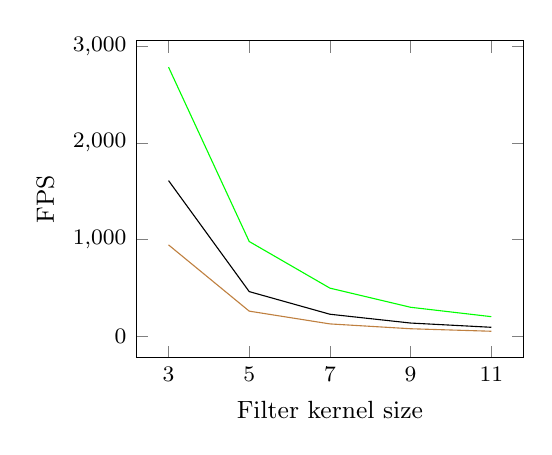
\begin{tikzpicture}
            \begin{axis}[
                small,
                xlabel={Filter kernel size},
                ylabel={FPS},
                xtick={3,5,7,9,11},
                xticklabels={3,5,7,9,11},
                % legend style={
                %     overlay,
                %     at={(1.25,0.5)},
                %     anchor=center},
                y tick label style={
                    /pgf/number format/.cd,
                        fixed,   % po zakomentowaniu os rzednych jest indeksowana wykladniczo
                        fixed, % 1.0 zamiast 1
                        precision=1,
                    /tikz/.cd
                },
                x tick label style={
                    /pgf/number format/.cd,
                        fixed,
                        fixed,
                        precision=2,
                    /tikz/.cd
                }
                ]
                \addplot [color=green]
                coordinates {
                    (3,2783)(5,980)(7,498)(9,300)(11,203)}; %\addlegendentry{720p}
                \addplot [color=black]
                coordinates {
                    (3,1610)(5,462)(7,228)(9,137)(11,93)}; %\addlegendentry{1080p}
                \addplot [color=brown]
                coordinates {
                    (3,945)(5,260)(7,128)(9,78)(11,52)}; %\addlegendentry{2k}
            \end{axis} 
        \end{tikzpicture}
        \caption{Results for the \textit{Cube} scene.}
        \label{fig:plot:pcf_cube}
    \end{subfigure}

    \vspace{20pt}
    \begin{subfigure}[t]{0.48\textwidth}
        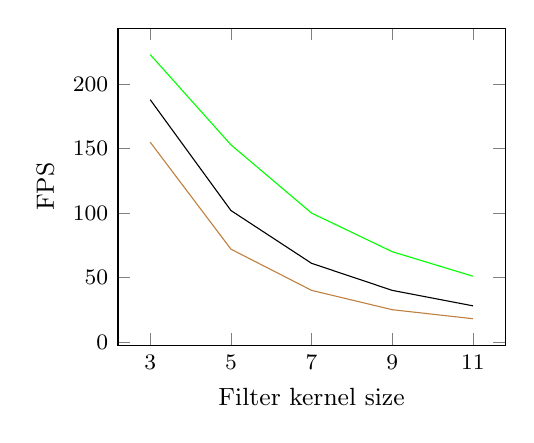
\begin{tikzpicture}
            \begin{axis}[
                small,
                xlabel={Filter kernel size},
                ylabel={FPS},
                xtick={3,5,7,9,11},
                xticklabels={3,5,7,9,11},
                % legend style={
                %     overlay,
                %     at={(1.25,0.5)},
                %     anchor=center},
                y tick label style={
                    /pgf/number format/.cd,
                        fixed,   % po zakomentowaniu os rzednych jest indeksowana wykladniczo
                        fixed, % 1.0 zamiast 1
                        precision=1,
                    /tikz/.cd
                },
                x tick label style={
                    /pgf/number format/.cd,
                        fixed,
                        fixed,
                        precision=2,
                    /tikz/.cd
                }
                ]
                \addplot [color=green]
                coordinates {
                    (3,223)(5,153)(7,100)(9,70)(11,51)}; %\addlegendentry{720p}
                \addplot [color=black]
                coordinates {
                    (3,188)(5,102)(7,61)(9,40)(11,28)}; %\addlegendentry{1080p}
                \addplot [color=brown]
                coordinates {
                    (3,155)(5,72)(7,40)(9,25)(11,18)}; %\addlegendentry{2k}
            \end{axis} 
        \end{tikzpicture}
        \caption{Results for the \textit{Power Plant} scene.}
        \label{fig:plot:pcf_power}
    \end{subfigure}
    \hfill
    \begin{subfigure}[t]{0.48\textwidth}
        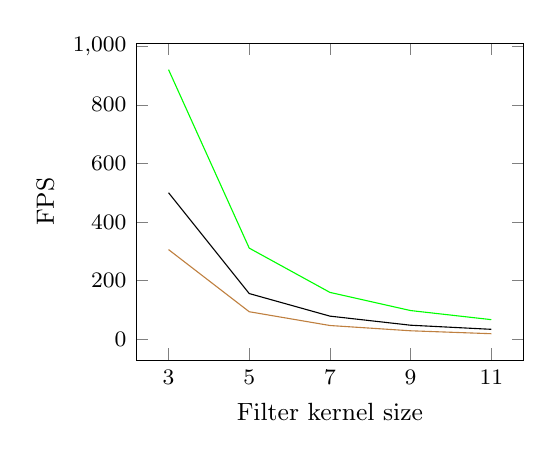
\begin{tikzpicture}
            \begin{axis}[
                small,
                xlabel={Filter kernel size},
                ylabel={FPS},
                xtick={3,5,7,9,11},
                xticklabels={3,5,7,9,11},
                % legend style={
                %     overlay,
                %     at={(1.25,0.5)},
                %     anchor=center},
                y tick label style={
                    /pgf/number format/.cd,
                        fixed,   % po zakomentowaniu os rzednych jest indeksowana wykladniczo
                        fixed, % 1.0 zamiast 1
                        precision=1,
                    /tikz/.cd
                },
                x tick label style={
                    /pgf/number format/.cd,
                        fixed,
                        fixed,
                        precision=2,
                    /tikz/.cd
                }
                ]
                \addplot [color=green]
                coordinates {
                    (3,920)(5,311)(7,160)(9,98)(11,67)}; %\addlegendentry{720p}
                \addplot [color=black]
                coordinates {
                    (3,500)(5,156)(7,79)(9,48)(11,34)}; %\addlegendentry{1080p}
                \addplot [color=brown]
                coordinates {
                    (3,306)(5,94)(7,47)(9,29)(11,19)}; %\addlegendentry{2k}
            \end{axis} 
        \end{tikzpicture}
        \caption{Results for the \textit{Crytek Sponza} scene.}
        \label{fig:plot:pcf_sponza}
    \end{subfigure}
    \caption{Frames per second for all test scenes, for different sizes of the filter kernel and output resolutions. In green \(1280\times 720\), in black \(1920\times 1080\) and in brown \(2560\times 1440\). Rendering with the basic shadow mapping technique with PCF at constant shadow map size \(1024\times 1024\).}
    \label{fig:plot:pcf_results}
\end{figure}

The results show performance dropping exponentially with regard to increasing filter kernel size. This is expected, as for a kernel of size \(n\) there are \(n^2\) depth comparisons performed per output pixel. This fact makes high kernel sizes impractical and limits the usability of the approach. A larger smoothing effect is better achieved by using a scale factor to scale the sample offsets within the filter kernel than by increasing the kernel size.

\begin{figure}[p]
    \centering
    \begin{subfigure}[t]{0.48\textwidth}
		\centering
        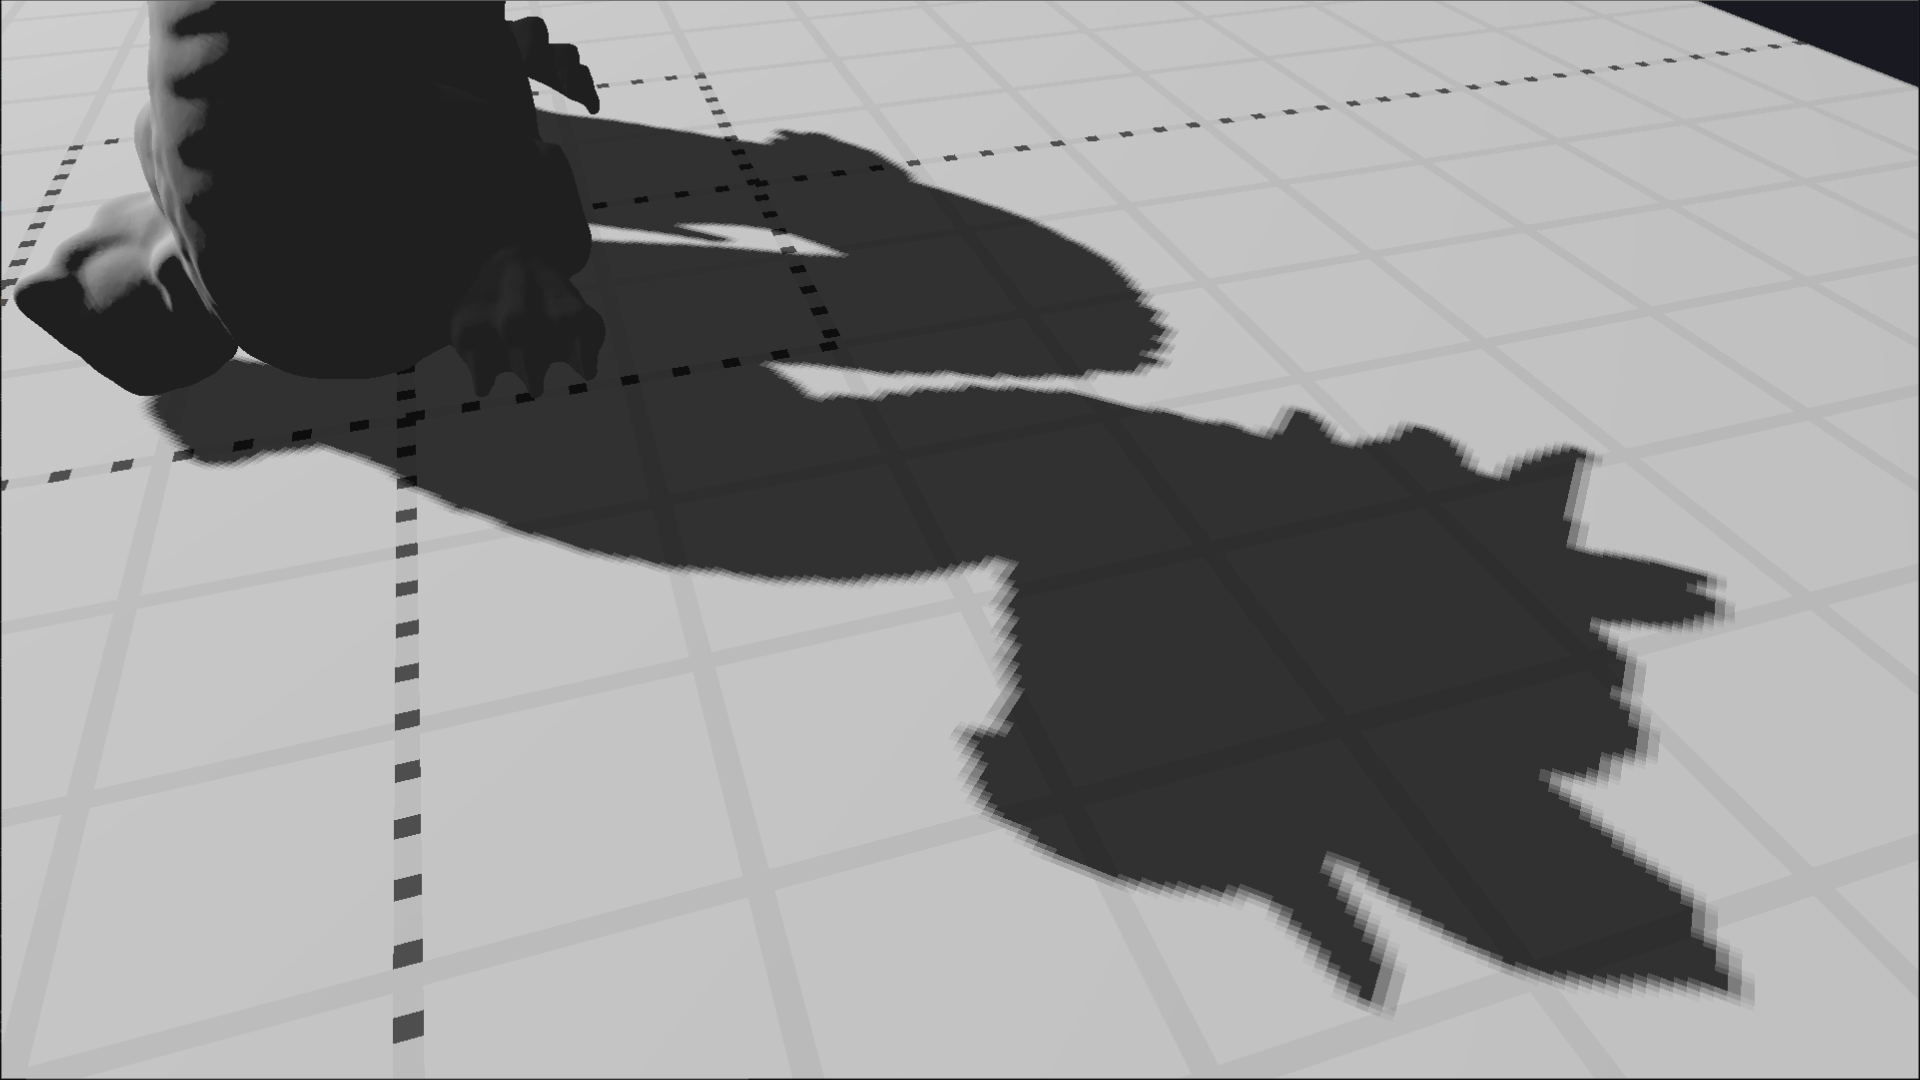
\includegraphics[width=\textwidth]{./graf/tests/pcf/cropped/dragon_pcf_fhd_1024_3x3.png}
        \caption{The shadow of the \textit{Chinese Dragon} filtered with a \(3\times 3\) kernel.}
    \end{subfigure}
	\hfill
    \begin{subfigure}[t]{0.48\textwidth}
		\centering
        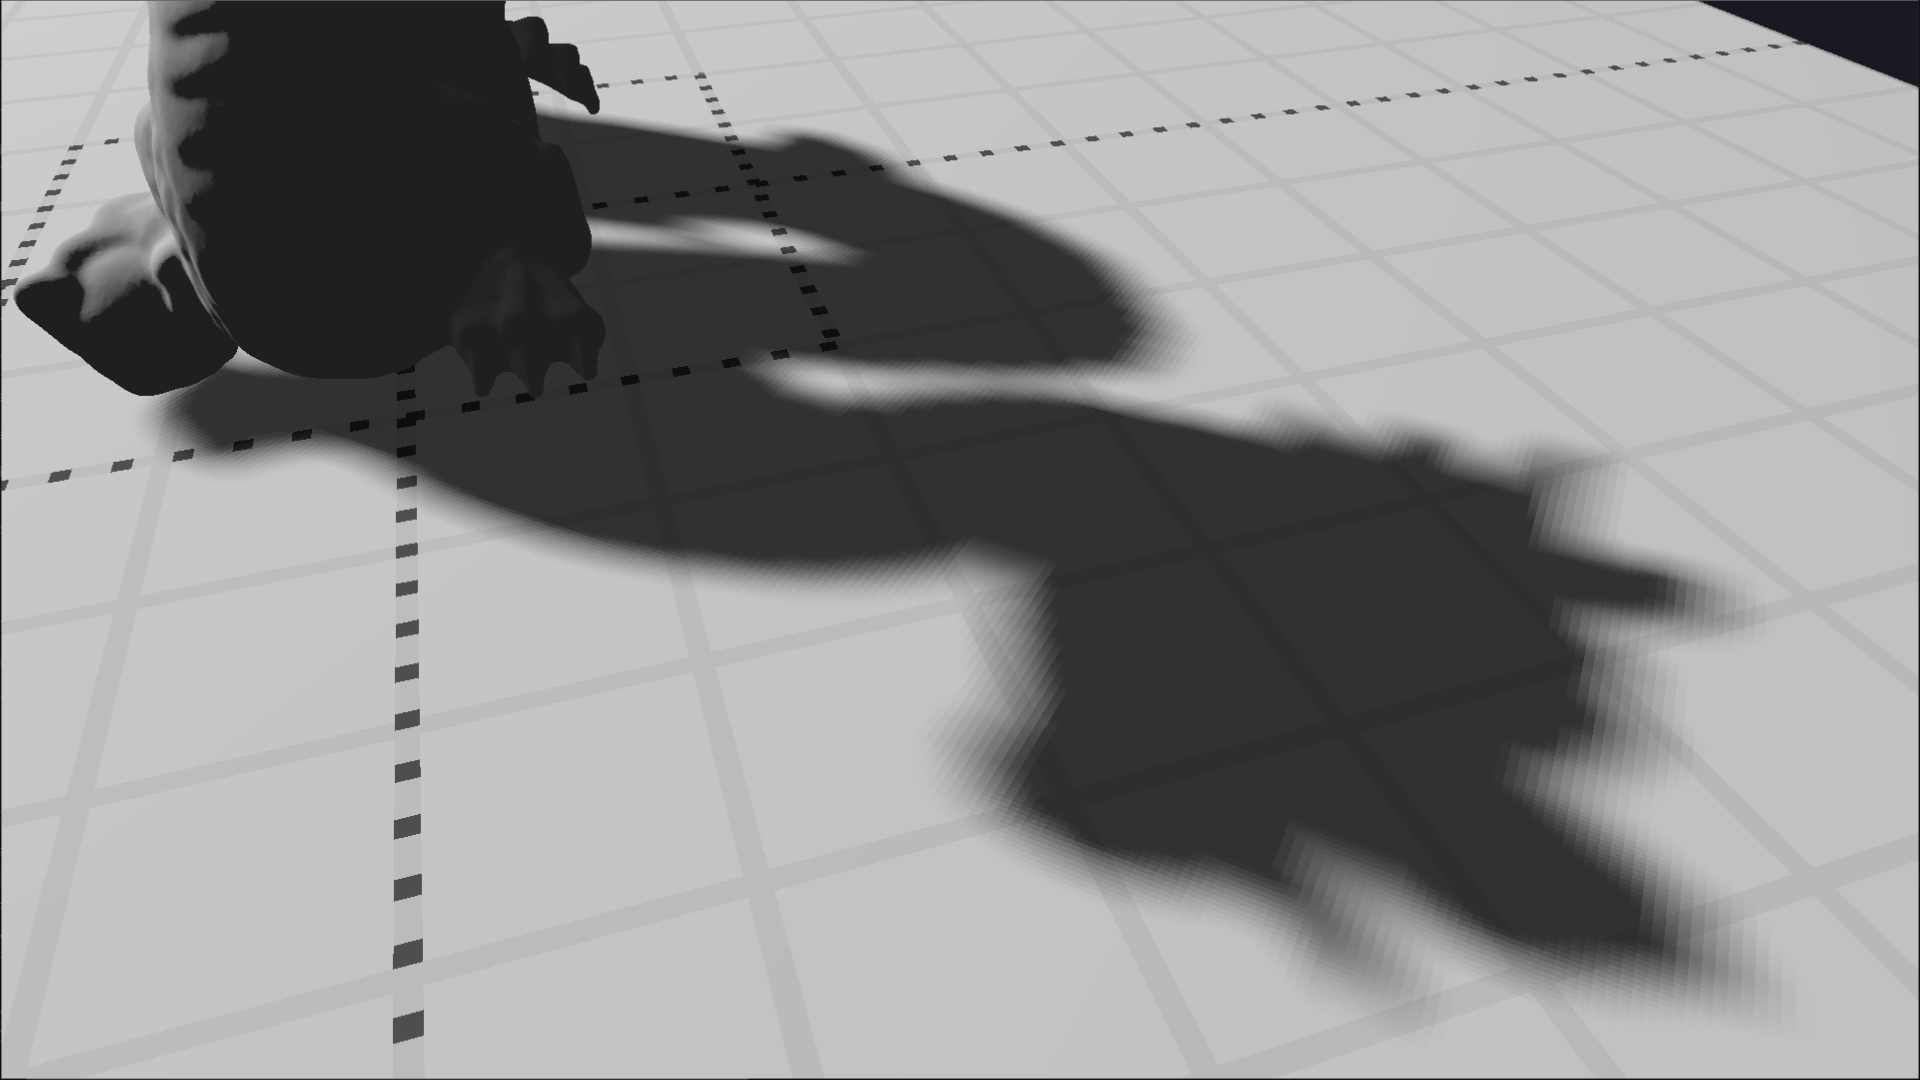
\includegraphics[width=\textwidth]{./graf/tests/pcf/cropped/dragon_pcf_fhd_1024_11x11.png}
        \caption{The shadow of the \textit{Chinese Dragon} filtered with an \(11\times 11\) kernel.}
    \end{subfigure}

    \begin{subfigure}[t]{0.48\textwidth}
		\centering
        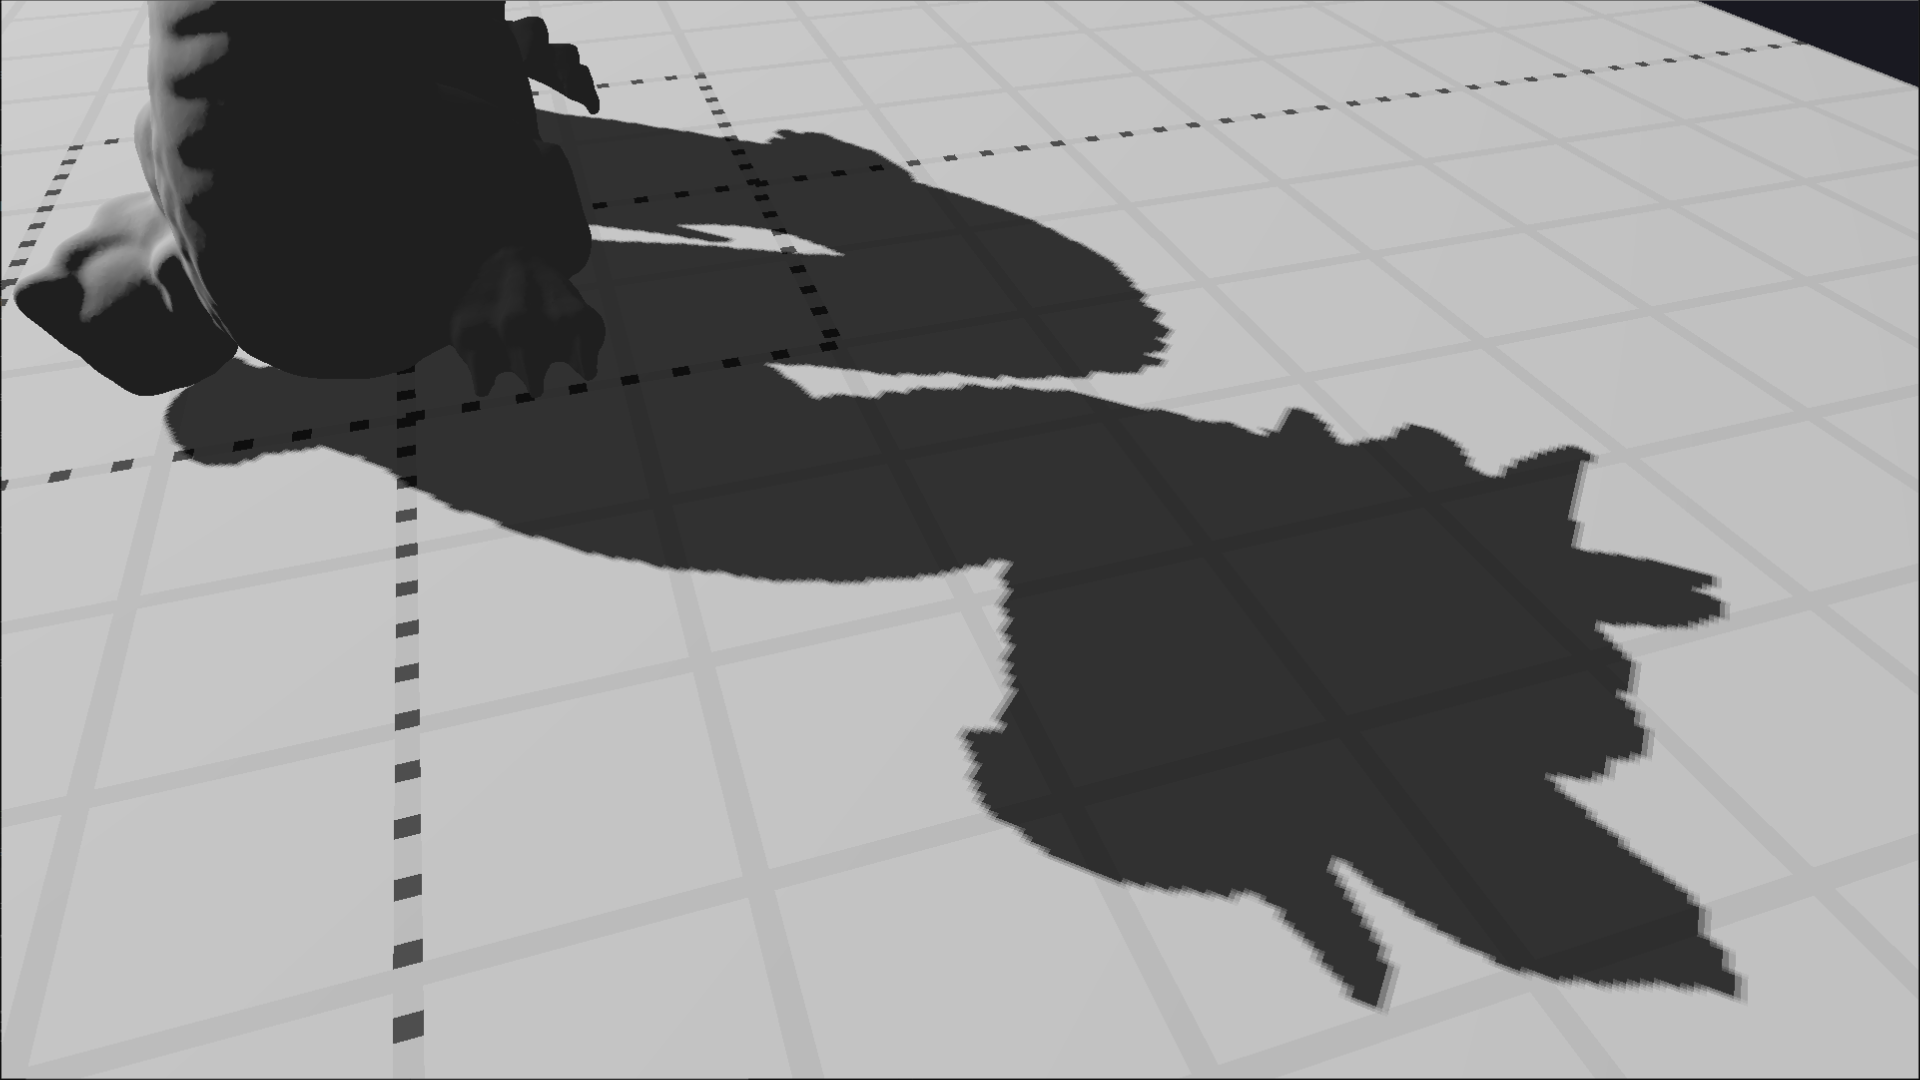
\includegraphics[width=\textwidth]{./graf/tests/pcf/cropped/dragon_pcf_fhd_1024_3x3_offset05.png}
        \caption{The shadow of the \textit{Chinese Dragon} filtered with a \(3\times 3\) kernel and a scale of \(0.5\) applied to each kernel offset.}
    \end{subfigure}
    \hfill
    \begin{subfigure}[t]{0.48\textwidth}
		\centering
        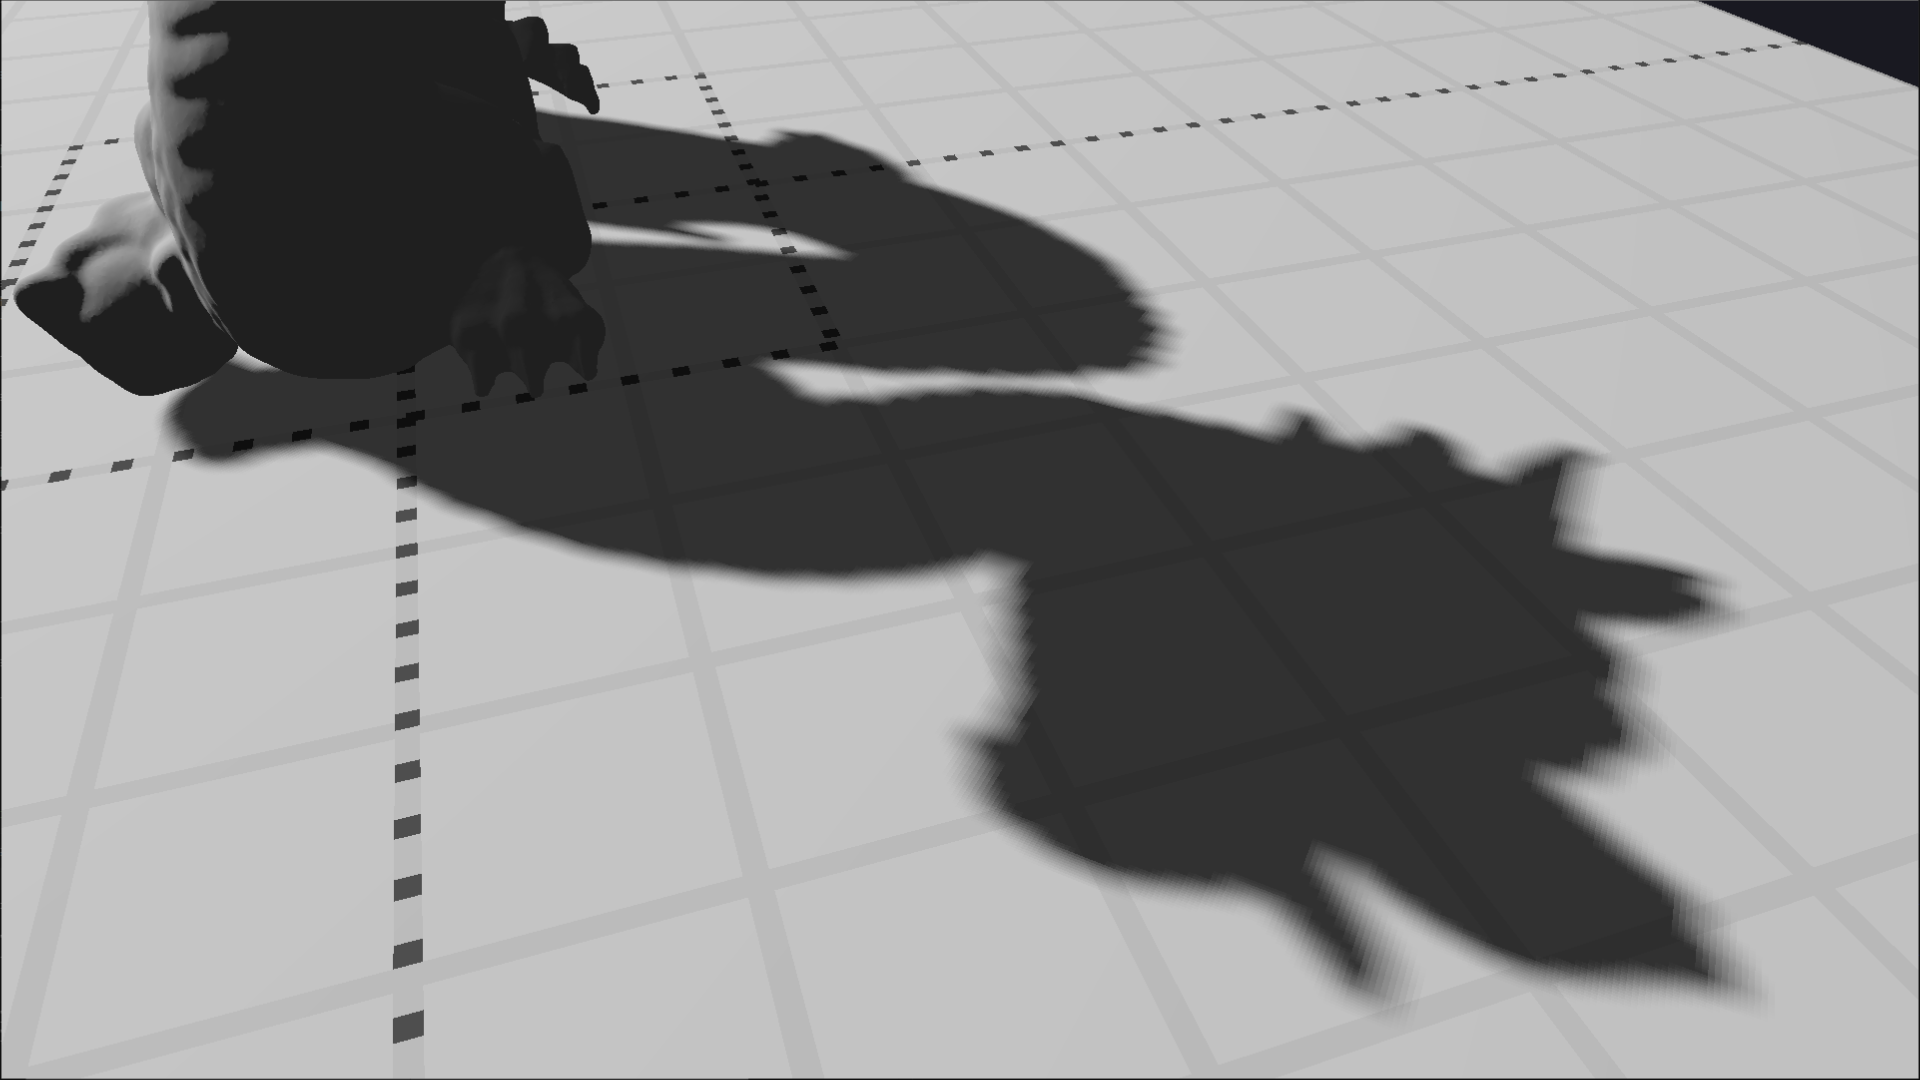
\includegraphics[width=\textwidth]{./graf/tests/pcf/cropped/dragon_pcf_fhd_1024_11x11_offset05.png}
        \caption{The shadow of the \textit{Chinese Dragon} filtered with an \(11\times 11\) kernel and a scale of \(0.5\) applied to each kernel offset.}
    \end{subfigure}

    \begin{subfigure}[t]{0.48\textwidth}
		\centering
        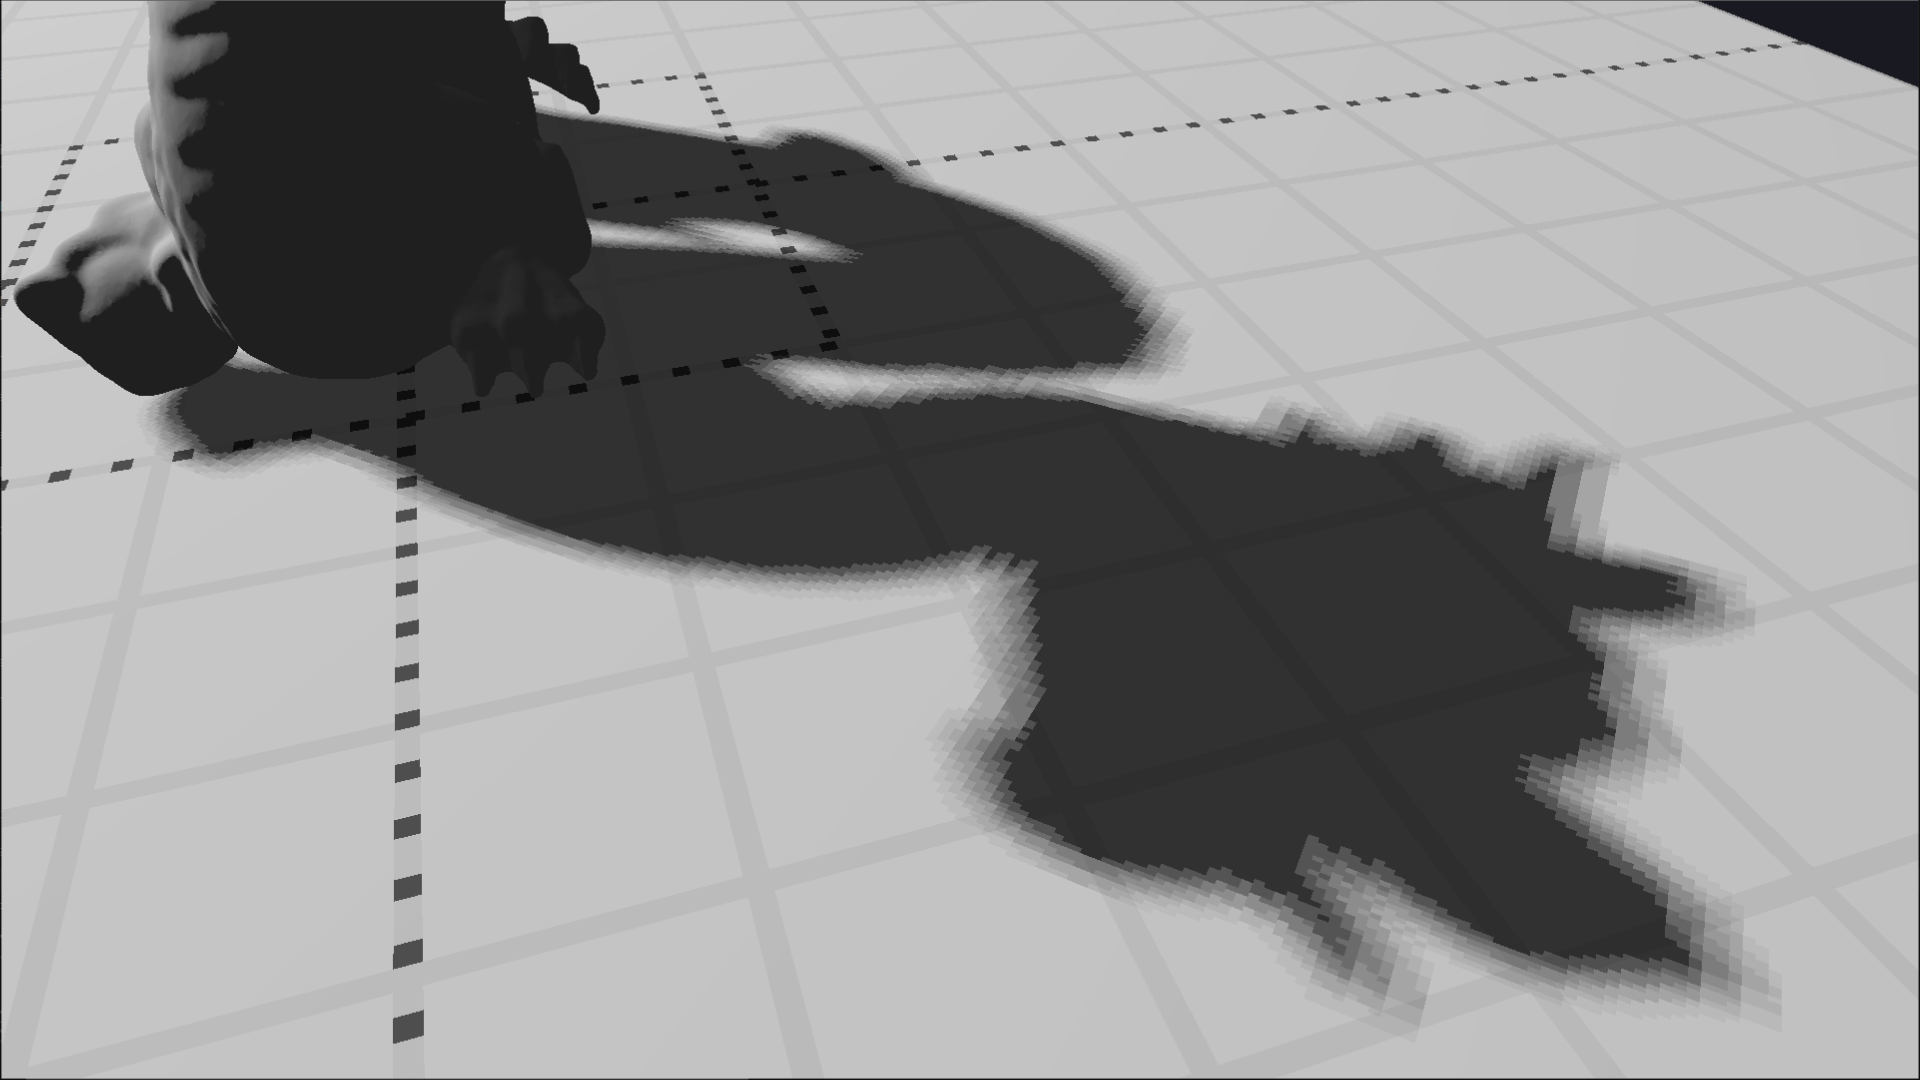
\includegraphics[width=\textwidth]{./graf/tests/pcf/cropped/dragon_pcf_fhd_1024_3x3_offset3.png}
        \caption{The shadow of the \textit{Chinese Dragon} filtered with a \(3\times 3\) kernel and a scale of \(3\) applied to each kernel offset.}
    \end{subfigure}
	\hfill
    \begin{subfigure}[t]{0.48\textwidth}
		\centering
        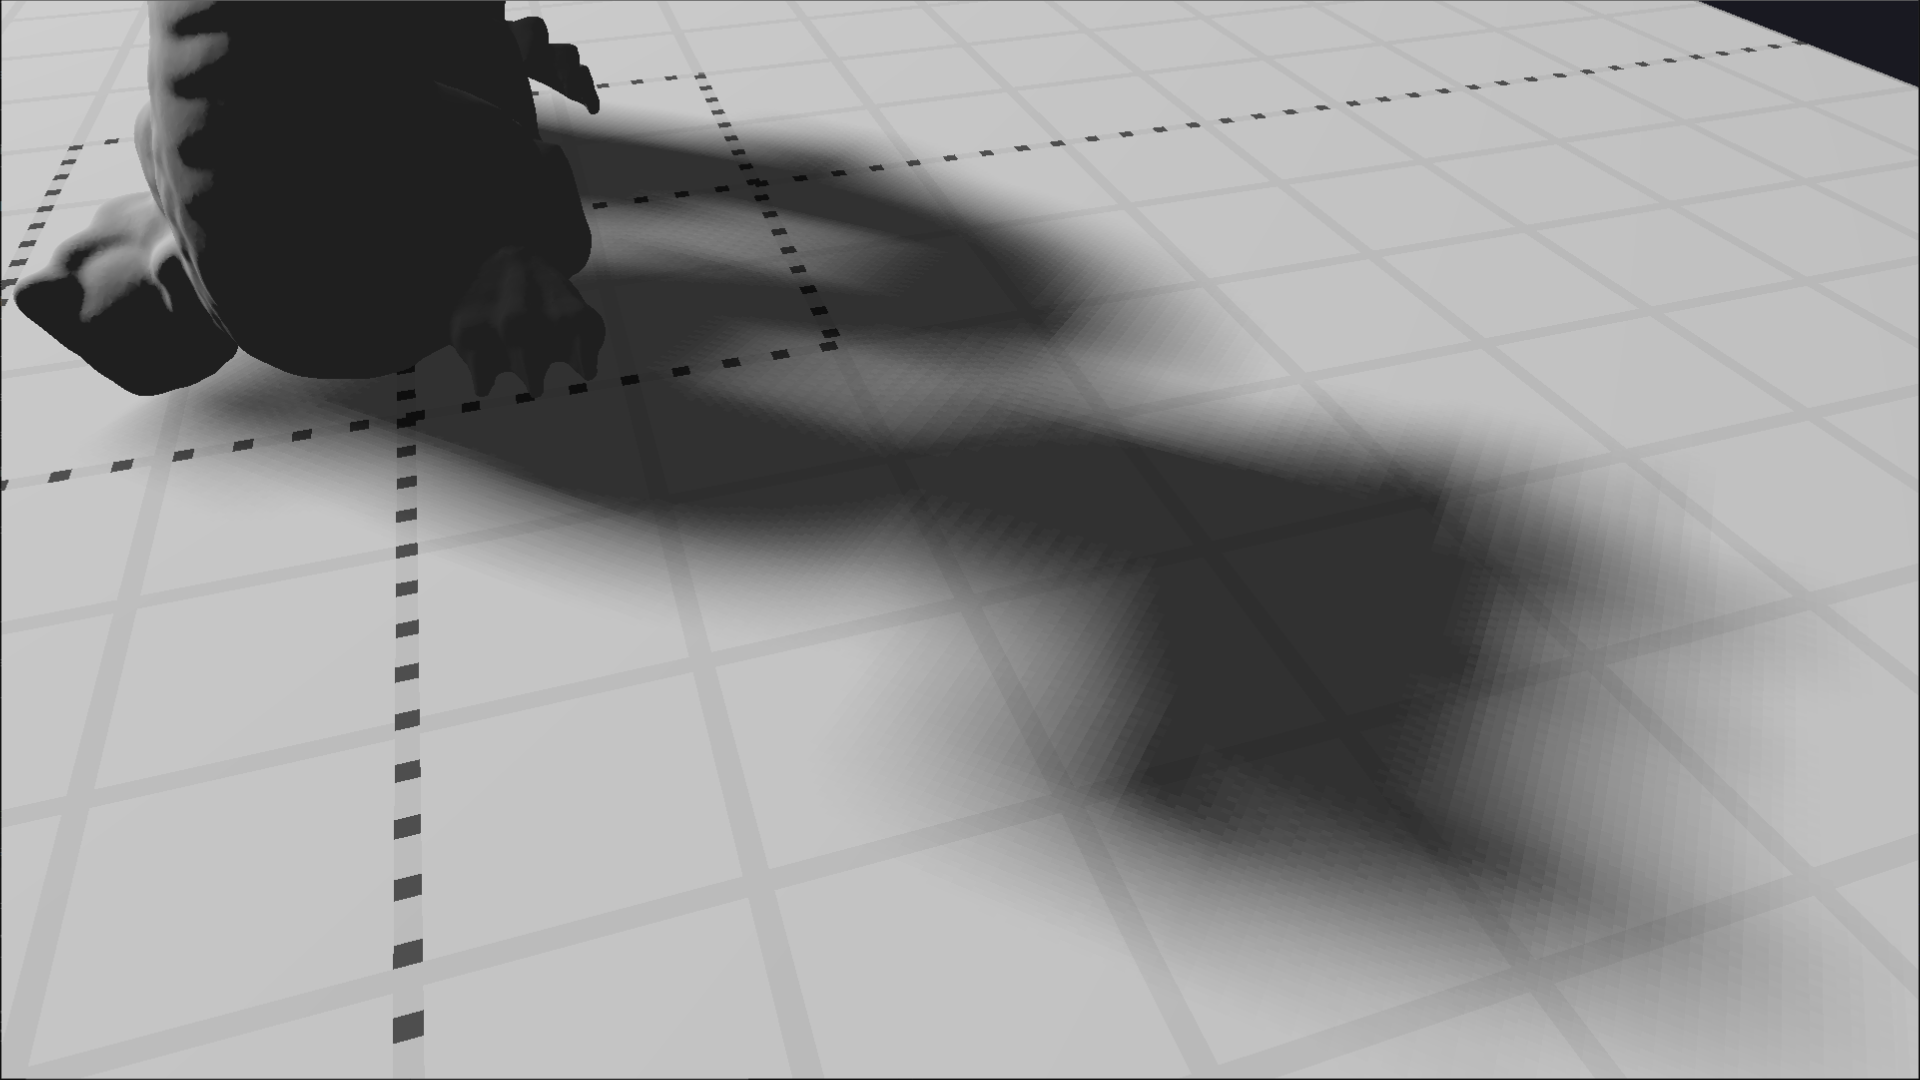
\includegraphics[width=\textwidth]{./graf/tests/pcf/cropped/dragon_pcf_fhd_1024_11x11_offset3.png}
        \caption{The shadow of the \textit{Chinese Dragon} filtered with an \(11\times 11\) kernel and a scale of \(3\) applied to each kernel offset.}
    \end{subfigure}    

    \caption{The \textit{Chinese Dragon} rendered with \(3\times 3\) and \(11\times 11\) kernels with different offset scales.}
    \label{fig:test_pcf_dragon_screens}
\end{figure}

During testing interesting behavior was observed. In all tests, when the application was running with its initial kernel parameter unchanged, the frame rate would be much higher than at the same kernel size after any change to it was made. This difference in some cases was as large as the entire FPS value after a change, meaning the loss of half the frame rate. The reason for this is not known, because default initialization and optimization of the code path is unlikely, as neither the shader code nor the compiler know of the initial settings that will be used for the kernel size. All results shown in Fig. \ref{fig:plot:pcf_results} present FPS values after the initial change was made.

The appearance of shadows rendered with different sizes of kernels and offsets is presented in Fig. \ref{fig:test_pcf_dragon_screens}.
Banding is very much visible in the smoothed areas of the shadows, even with the largest kernel. This is because of the limited range of shades that can be produced in these transitional areas. A transition that appears smoother can be achieved by setting a smaller than 1 offset scale, but that limits the size of the smoothed shadow areas. Additionally, texel boundaries are always visible with this method.

The usage of even the smallest \(3\times 3\) kernel requires adjusting the depth bias to get clean results. The larger the kernel, the more bias is needed. This could be partially alleviated by using the distance from the kernel center to scale a bias that is added before the comparison happens, but overall bias would still depend on receiver orientations and would need to be adjusted per-scene.

\begin{figure}[h]
    \centering
    \begin{subfigure}[t]{0.45\textwidth}
		\centering
        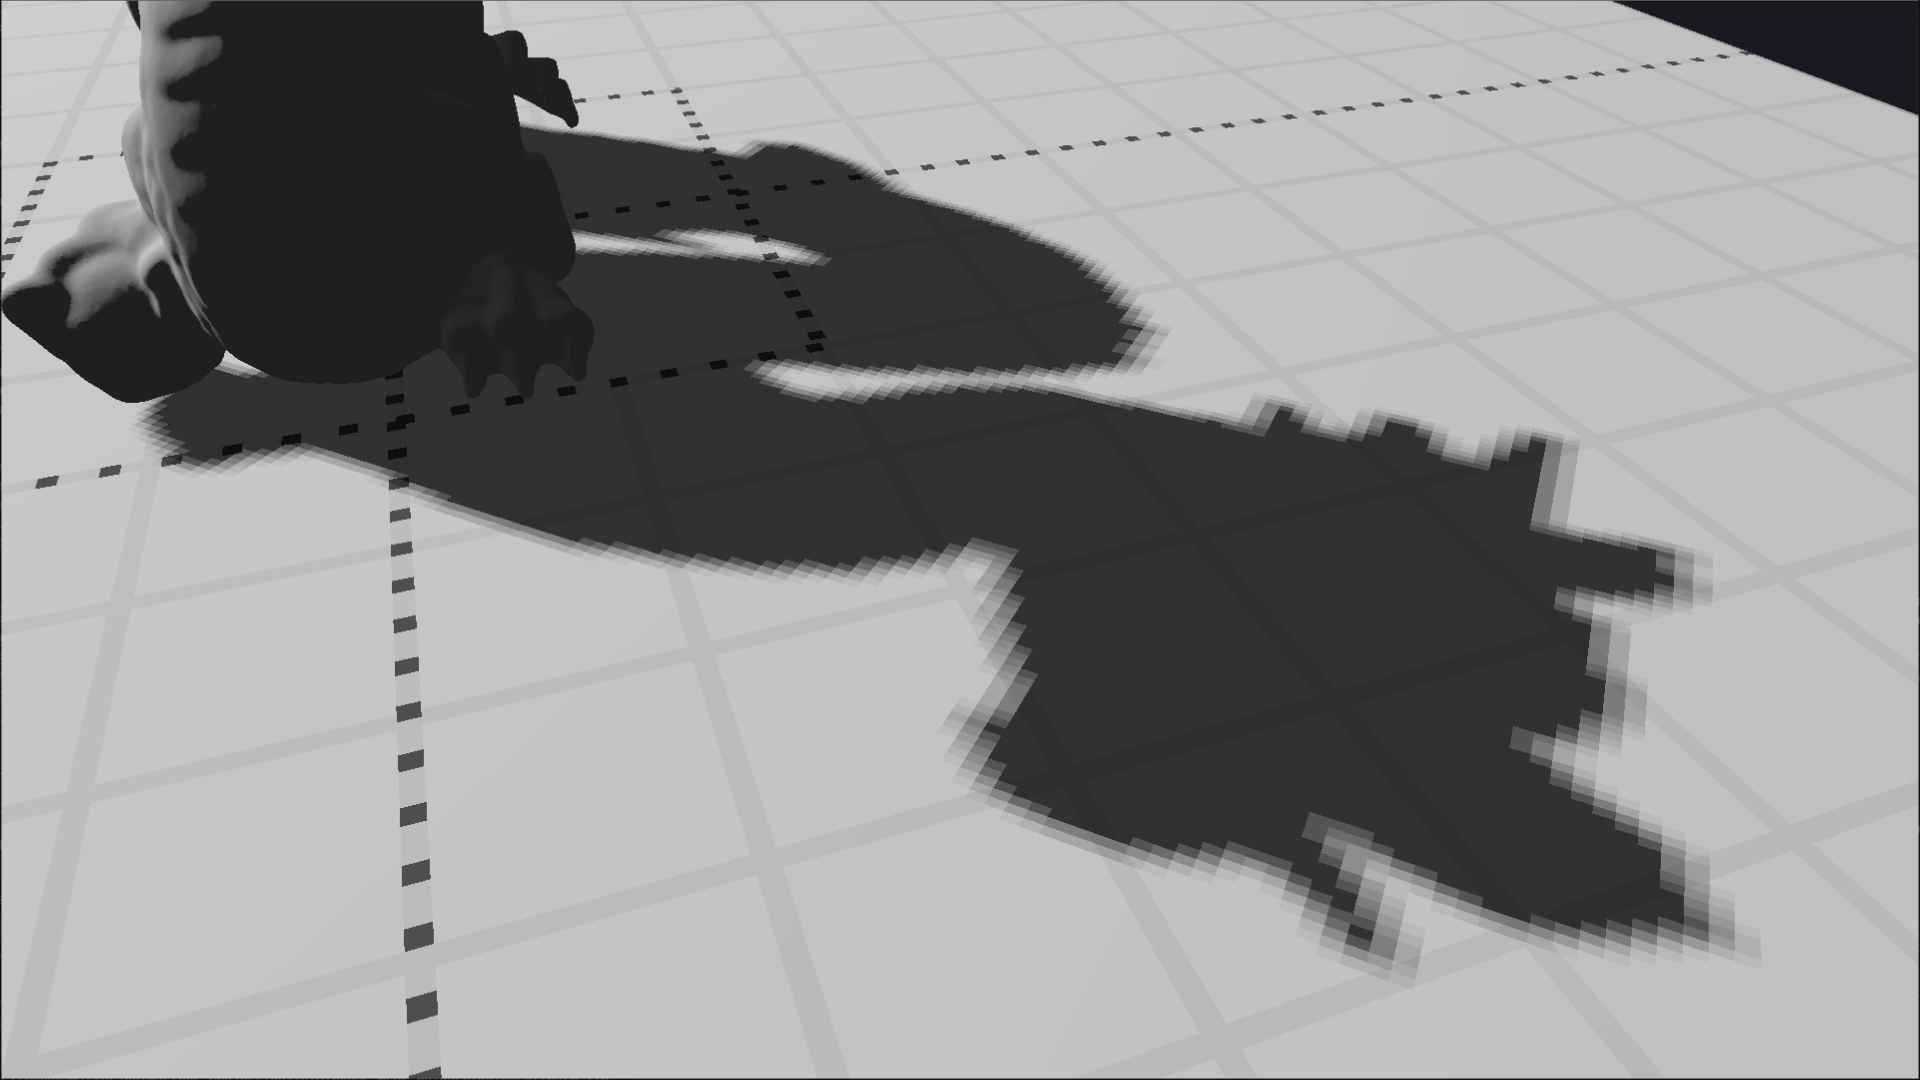
\includegraphics[width=\textwidth]{./graf/tests/pcf/cropped/dragon_pcf_fhd_512_3x3.png}
        \caption{The \textit{Chinese Dragon} rendered with basic \(3\times 3\) PCF.}
    \end{subfigure}
	\hfill
    \begin{subfigure}[t]{0.45\textwidth}
		\centering
        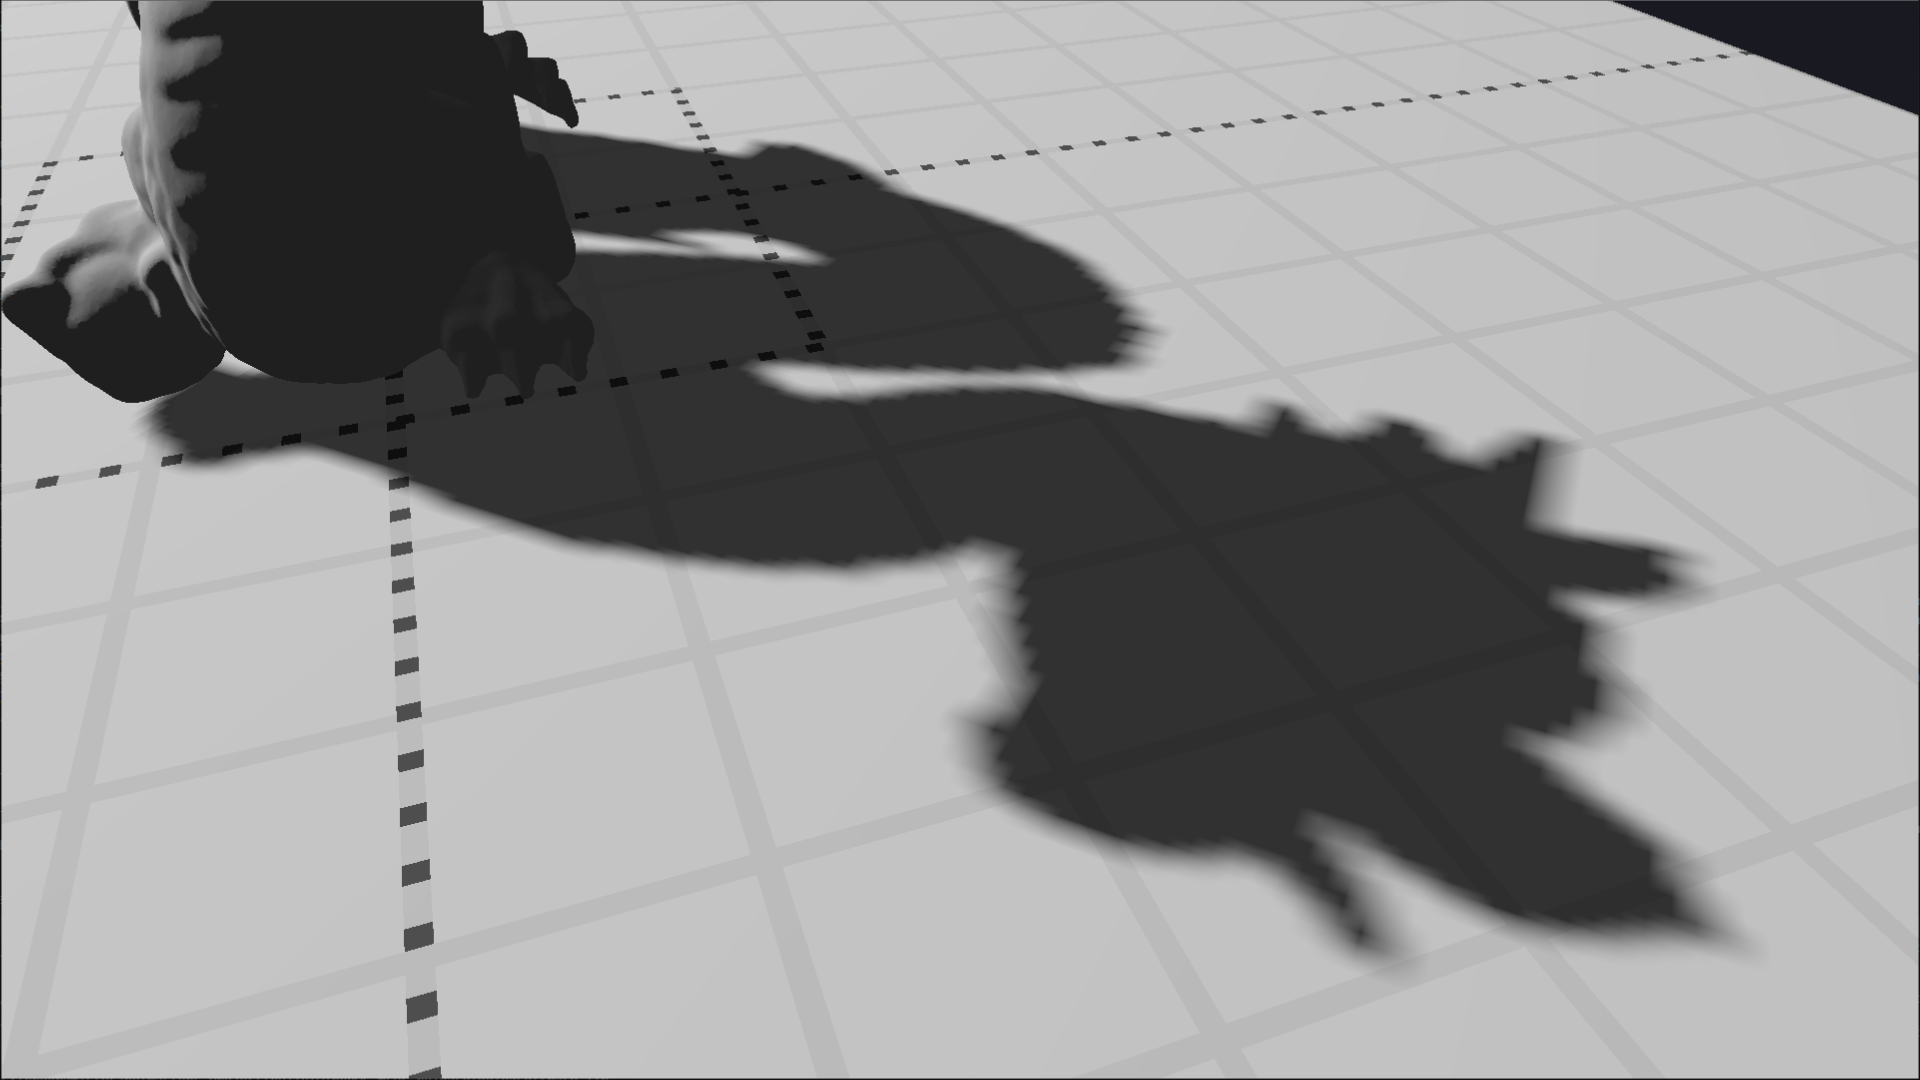
\includegraphics[width=\textwidth]{./graf/tests/pcf/cropped/dragon_pcf_fhd_512_3x3_bilinear.png}
        \caption{The \textit{Chinese Dragon} rendered with \(3\times 3\) PCF enhanced by bilinear filtering.}
    \end{subfigure}
    \begin{subfigure}[t]{0.45\textwidth}
		\centering
        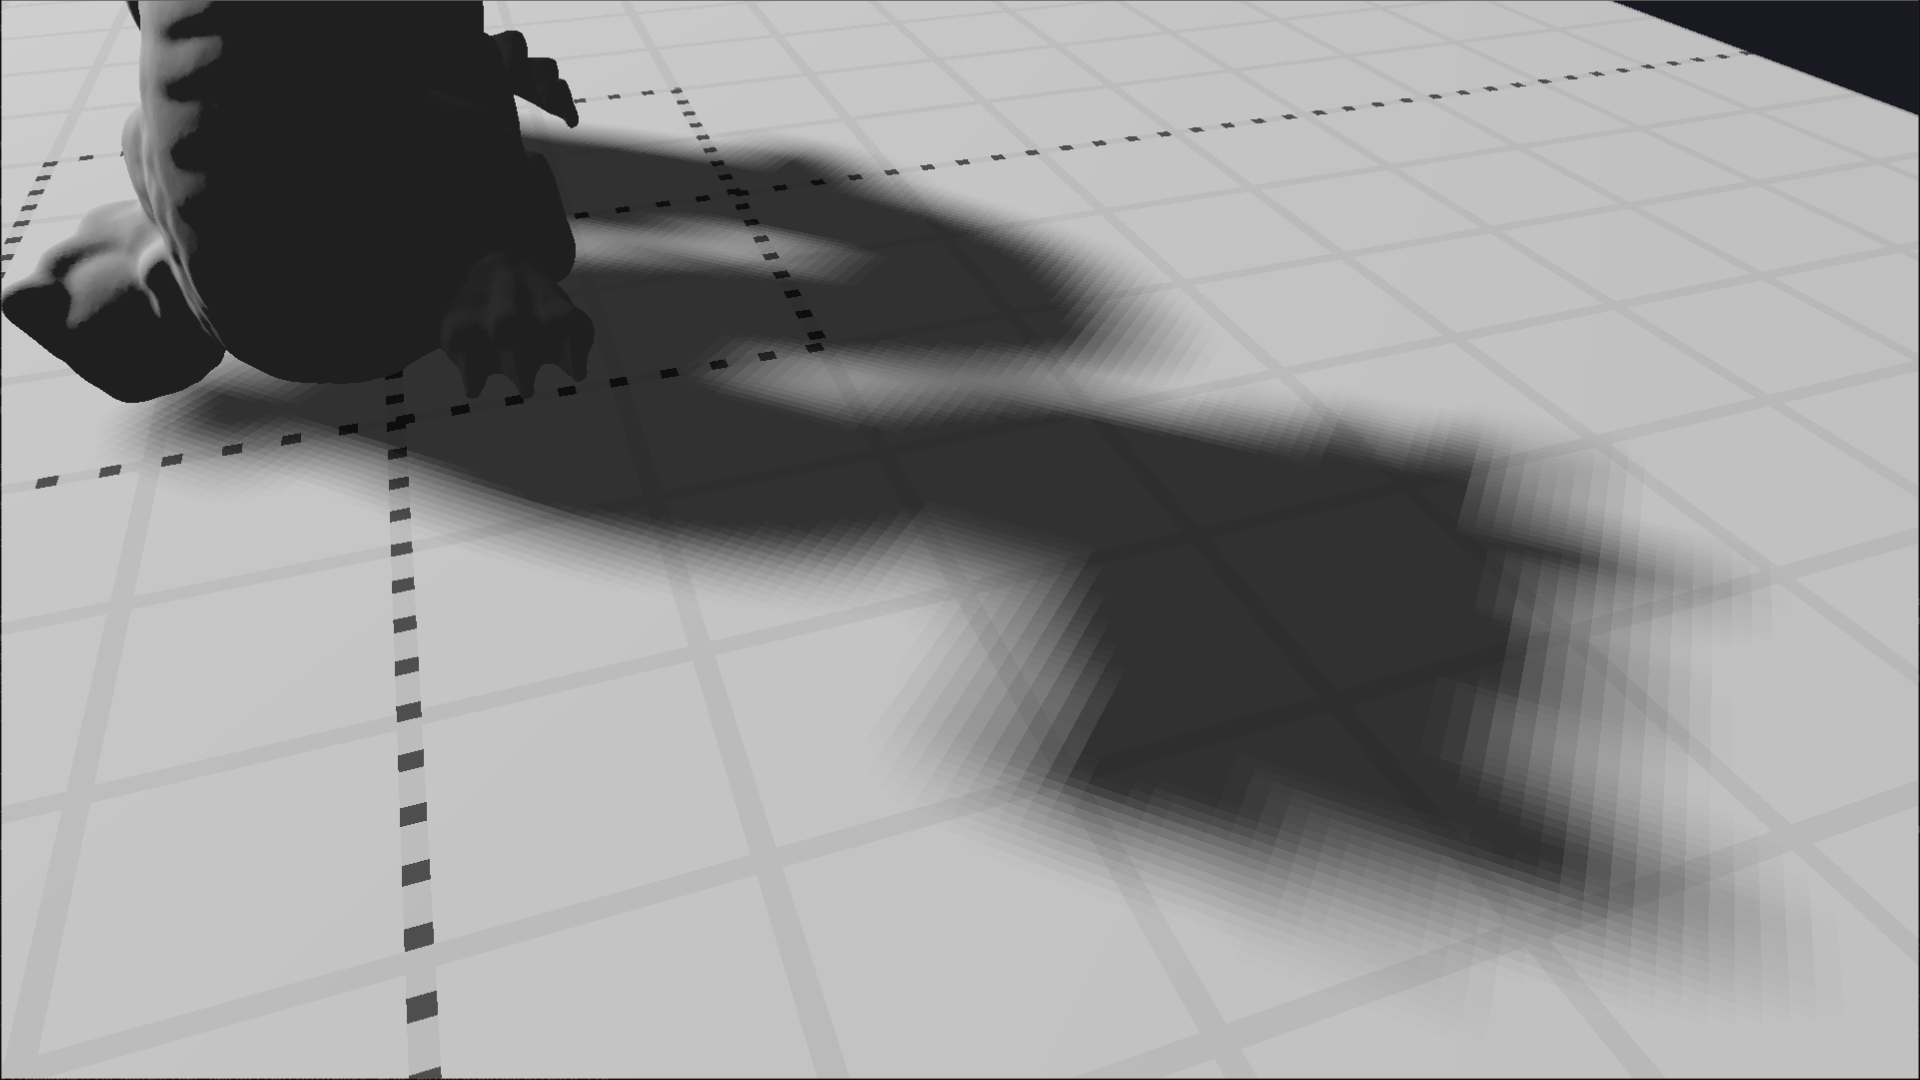
\includegraphics[width=\textwidth]{./graf/tests/pcf/cropped/dragon_pcf_fhd_512_11x11.png}
        \caption{The \textit{Chinese Dragon} rendered with basic \(11\times 11\) PCF.}
    \end{subfigure}
	\hfill
    \begin{subfigure}[t]{0.45\textwidth}
		\centering
        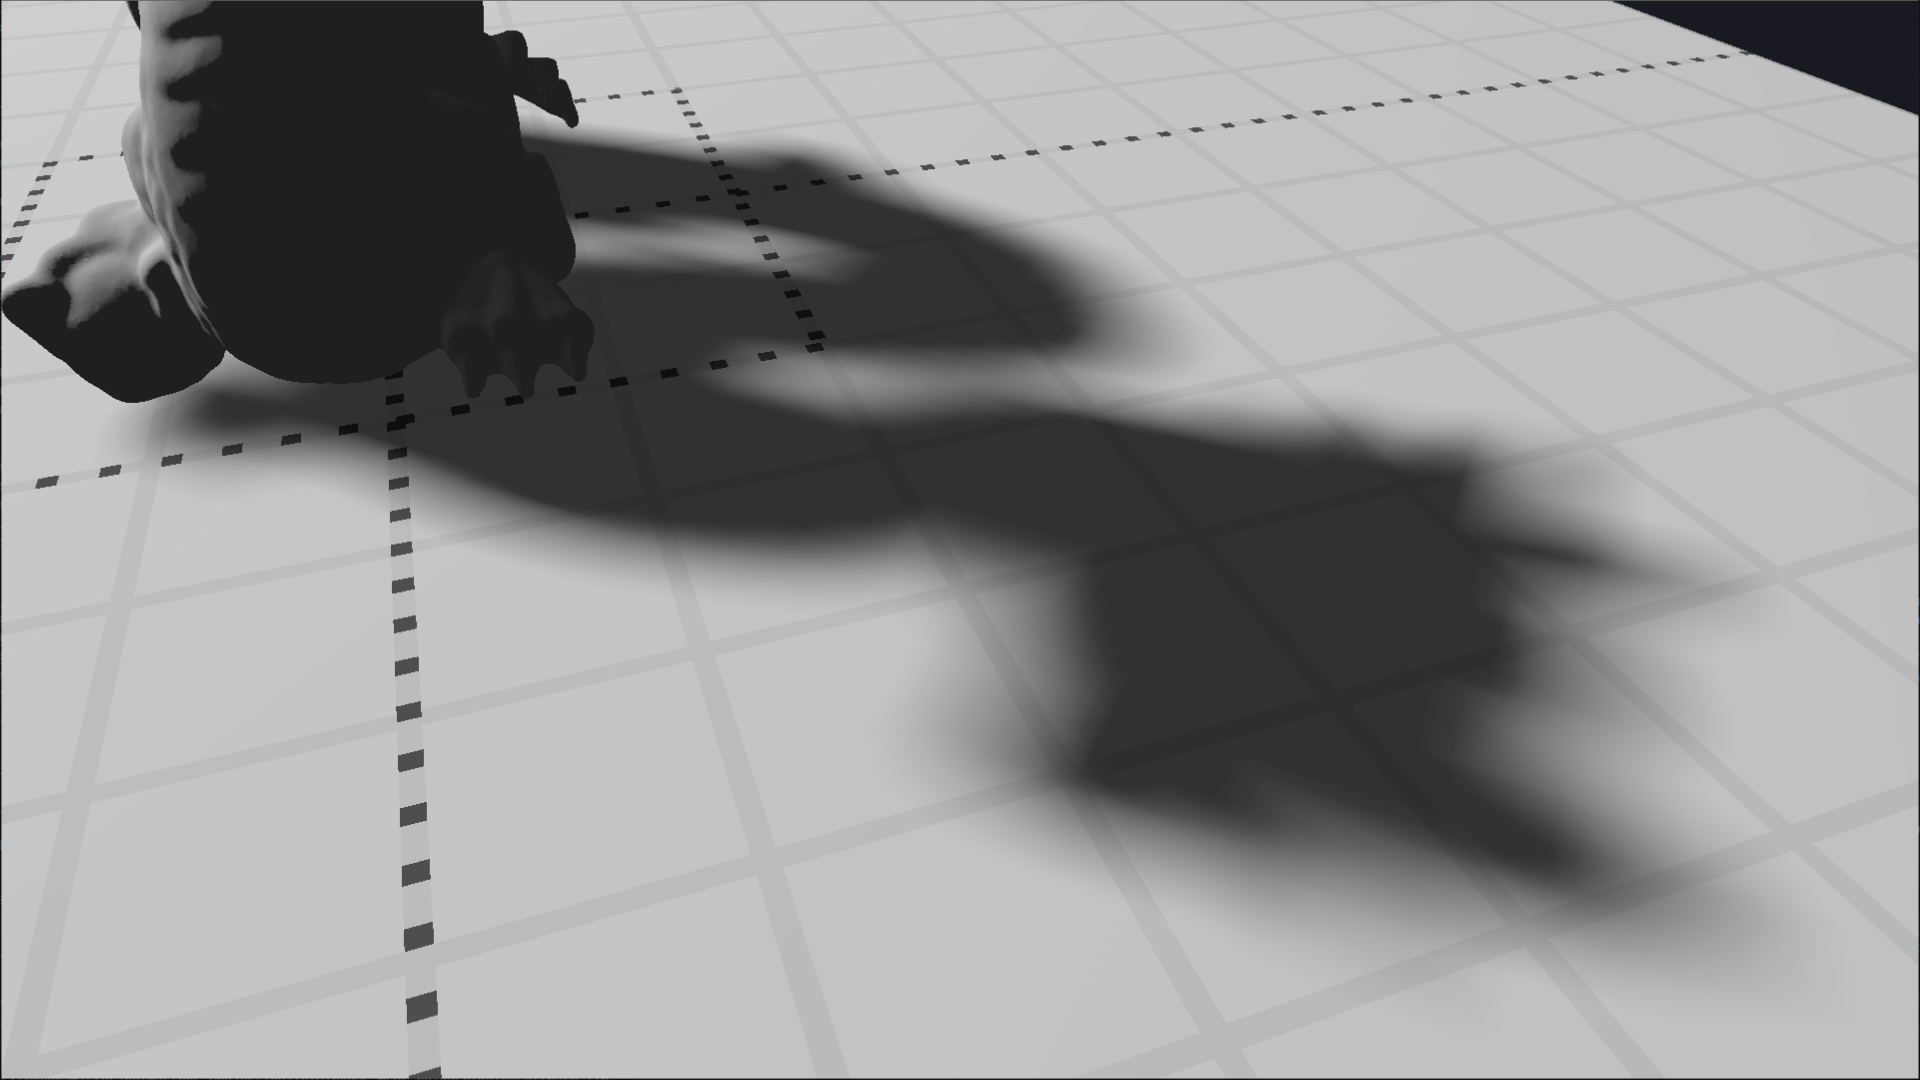
\includegraphics[width=\textwidth]{./graf/tests/pcf/cropped/dragon_pcf_fhd_512_11x11_bilinear.png}
        \caption{The \textit{Chinese Dragon} rendered with \(11\times 11\) PCF enhanced by bilinear filtering.}
    \end{subfigure}

    \caption{The \textit{Chinese Dragon} rendered with PCF and with and without additional bilinear comparison filtering, using a \(512\times 512\) shadow map resolution.}
    \label{fig:test_pfc_bilinear_dragon_screens}
\end{figure}

The performance cost and underwhelming results make this technique mainly a stepping stone for more robust approaches. It is not practical to use it in real applications that need to run in real-time. There is however one adjustment that can be made to significantly improve the shadow's appearance produced by PCF. As established in section \ref{section:test_bilinear}, hardware bilinear comparison filtering comes at virtually no performance cost. It can be applied to PCF, the results of which are shown in Fig. \ref{fig:test_pfc_bilinear_dragon_screens}

These results show that bilinear comparison filtering combined with PCF can lead to a great improvement of the visuals, even at kernel sizes as small as \(3\times 3\). Additionally, the shadow map used there has only \(512\times 512\) resolution, making it a very performant option. The impractical kernel size \(11\times 11\), when combined with bilinear filtering gives very smooth results, without any banding, hiding the texel boundaries very well, especially considering the low resolution of the shadow map.

\subsubsection{Adaptive percentage-closer filtering}
Adaptive PCF aims to improve the performance of regular PCF by allowing only some of the kernel samples to be processed when the shaded pixel in not in a penumbra region. It also improves the control over the penumbra size while maintaining visual quality. This is tested in this section, beginning with the results of performance testing presented in Fig. \ref{fig:plot:pcf_adaptive_results}.

\begin{figure}[h]
    \centering
    \begin{subfigure}[t]{0.48\textwidth}
        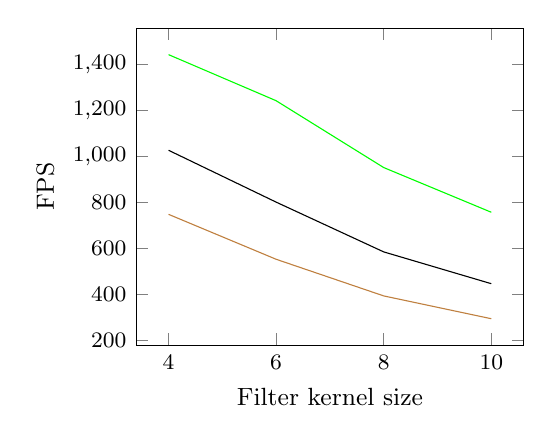
\begin{tikzpicture}
            \begin{axis}[
                small,
                xlabel={Filter kernel size},
                ylabel={FPS},
                xtick={4,6,8,10},
                xticklabels={4,6,8,10},
                % legend style={
                %     overlay,
                %     at={(1.25,0.5)},
                %     anchor=center},
                y tick label style={
                    /pgf/number format/.cd,
                        fixed,   % po zakomentowaniu os rzednych jest indeksowana wykladniczo
                        fixed, % 1.0 zamiast 1
                        precision=1,
                    /tikz/.cd
                },
                x tick label style={
                    /pgf/number format/.cd,
                        fixed,
                        fixed,
                        precision=2,
                    /tikz/.cd
                }
                ]
                \addplot [color=green]
                coordinates {
                    (4,1441)(6,1241)(8,951)(10,757)}; %\addlegendentry{720p}
                \addplot [color=black]
                coordinates {
                    (4,1026)(6,801)(8,585)(10,447)}; %\addlegendentry{1080p}
                \addplot [color=brown]
                coordinates {
                    (4,748)(6,553)(8,394)(10,295)}; %\addlegendentry{2k}
            \end{axis} 
        \end{tikzpicture}
        \caption{Results for the \textit{Chinese Dragon} scene.}
        \label{fig:plot:pcf_adaptive_dragon}
    \end{subfigure}
    \hfill
    \begin{subfigure}[t]{0.48\textwidth}
        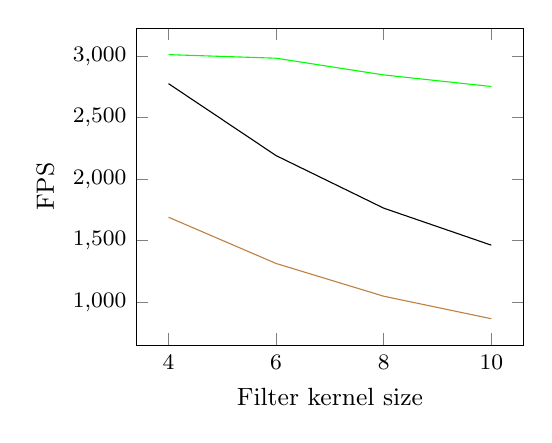
\begin{tikzpicture}
            \begin{axis}[
                small,
                xlabel={Filter kernel size},
                ylabel={FPS},
                xtick={4,6,8,10},
                xticklabels={4,6,8,10},
                % legend style={
                %     overlay,
                %     at={(1.25,0.5)},
                %     anchor=center},
                y tick label style={
                    /pgf/number format/.cd,
                        fixed,   % po zakomentowaniu os rzednych jest indeksowana wykladniczo
                        fixed, % 1.0 zamiast 1
                        precision=1,
                    /tikz/.cd
                },
                x tick label style={
                    /pgf/number format/.cd,
                        fixed,
                        fixed,
                        precision=2,
                    /tikz/.cd
                }
                ]
                \addplot [color=green]
                coordinates {
                    (4,3012)(6,2983)(8,2847)(10,2753)}; %\addlegendentry{720p}
                \addplot [color=black]
                coordinates {
                    (4,2776)(6,2191)(8,1764)(10,1463)}; %\addlegendentry{1080p}
                \addplot [color=brown]
                coordinates {
                    (4,1690)(6,1314)(8,1048)(10,865)}; %\addlegendentry{2k}
            \end{axis} 
        \end{tikzpicture}
        \caption{Results for the \textit{Cube} scene.}
        \label{fig:plot:pcf_adaptive_cube}
    \end{subfigure}

    \vspace{20pt}
    \begin{subfigure}[t]{0.48\textwidth}
        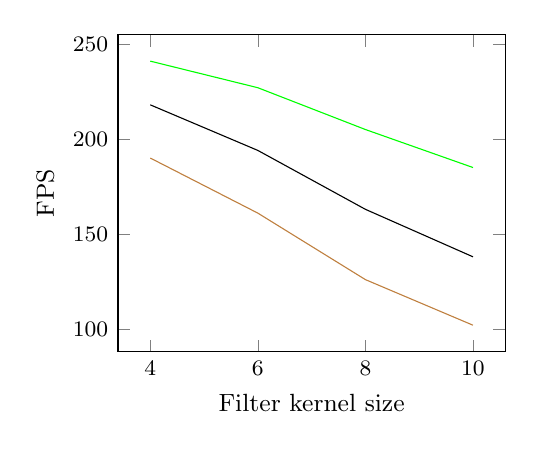
\begin{tikzpicture}
            \begin{axis}[
                small,
                xlabel={Filter kernel size},
                ylabel={FPS},
                xtick={4,6,8,10},
                xticklabels={4,6,8,10},
                % legend style={
                %     overlay,
                %     at={(1.25,0.5)},
                %     anchor=center},
                y tick label style={
                    /pgf/number format/.cd,
                        fixed,   % po zakomentowaniu os rzednych jest indeksowana wykladniczo
                        fixed, % 1.0 zamiast 1
                        precision=1,
                    /tikz/.cd
                },
                x tick label style={
                    /pgf/number format/.cd,
                        fixed,
                        fixed,
                        precision=2,
                    /tikz/.cd
                }
                ]
                \addplot [color=green]
                coordinates {
                    (4,241)(6,227)(8,205)(10,185)}; %\addlegendentry{720p}
                \addplot [color=black]
                coordinates {
                    (4,218)(6,194)(8,163)(10,138)}; %\addlegendentry{1080p}
                \addplot [color=brown]
                coordinates {
                    (4,190)(6,161)(8,126)(10,102)}; %\addlegendentry{2k}
            \end{axis} 
        \end{tikzpicture}
        \caption{Results for the \textit{Power Plant} scene.}
        \label{fig:plot:pcf_adaptive_power}
    \end{subfigure}
    \hfill
    \begin{subfigure}[t]{0.48\textwidth}
        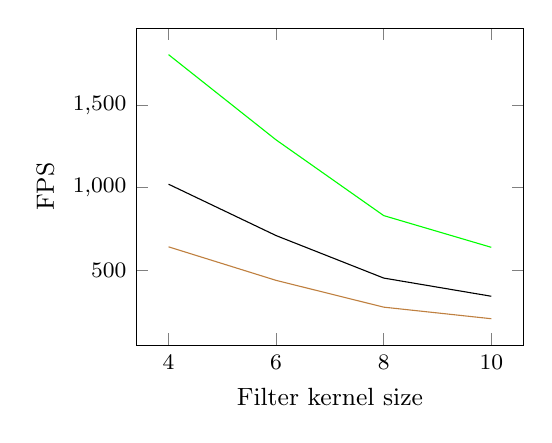
\begin{tikzpicture}
            \begin{axis}[
                small,
                xlabel={Filter kernel size},
                ylabel={FPS},
                xtick={4,6,8,10},
                xticklabels={4,6,8,10},
                % legend style={
                %     overlay,
                %     at={(1.25,0.5)},
                %     anchor=center},
                y tick label style={
                    /pgf/number format/.cd,
                        fixed,   % po zakomentowaniu os rzednych jest indeksowana wykladniczo
                        fixed, % 1.0 zamiast 1
                        precision=1,
                    /tikz/.cd
                },
                x tick label style={
                    /pgf/number format/.cd,
                        fixed,
                        fixed,
                        precision=2,
                    /tikz/.cd
                }
                ]
                \addplot [color=green]
                coordinates {
                    (4,1805)(6,1289)(8,831)(10,639)}; %\addlegendentry{720p}
                \addplot [color=black]
                coordinates {
                    (4,1021)(6,710)(8,453)(10,343)}; %\addlegendentry{1080p}
                \addplot [color=brown]
                coordinates {
                    (4,642)(6,439)(8,277)(10,207)}; %\addlegendentry{2k}
            \end{axis} 
        \end{tikzpicture}
        \caption{Results for the \textit{Crytek Sponza} scene.}
        \label{fig:plot:pcf_adaptive_sponza}
    \end{subfigure}
    \caption{Frames per second for all test scenes, for different sizes of the filter kernel and output resolutions. In green \(1280\times 720\), in black \(1920\times 1080\) and in brown \(2560\times 1440\). Rendering with the basic shadow mapping technique with adaptive PCF at constant shadow map size \(1024\times 1024\).}
    \label{fig:plot:pcf_adaptive_results}
\end{figure}

The produced graphs show that the technique does indeed improve performance in a significant way. Not only are the FPS higher, giving for the smallest kernel sizes \(15\%\) up to \(104\%\) more FPS depending on the scene, but the frame rate also falls off less rapidly with increasing kernel size, giving between \(392\%\) up to \(1473\%\) more FPS for the largest kernel sizes. This is a very meaningful performance boost, making this technique capable of real-time performance. This is owed to the fact that small kernels are used to determine if a position is in the penumbra region which needs to be smoothed, and filtering stops if it is not.
% for max kernel:
%     regular:
%         34 (sponza)
%         28
%         93
%         50 (dragon)
%     adaptive:
%         343 = 908% more fps
%         138 = 392% more fps
%         1463 = 1473
%         447 = 794

% for min kernel:
% regular:
%     500
%     188
%     1610
%     654
% adaptive:
%     1021 = 104% more
%     218 = 15% more
%     2776 = 72% more
%     1026 = 56% more

Because this optimization technique is adaptive, its performance is view dependent. More kernel samples will be used if the view contains large penumbra regions than when it only contains fully lit or fully shadowed surfaces. The FPS difference can be even that of \(50\%\). It can also vary depending on the scene for the same reason, so actual performance gains will vary. Performance will also be directly dependent on the sample offset scale, since with higher offsets larger penumbras are produced. This technique however will always give better or equal performance as basic PCF of the same kernel size.

As observed in previous tests, the bias has to be adjusted carefully when using filtering. In the case of adaptive PCF, a bad bias will not only result in degradation of the produced visuals but also degradation of performance, as more surface points will utilize the full kernel size when in the penumbra of an erroneous shadow.

Adaptive PCF in this implementation uses \(m\times m\) sets of randomized kernels. A specific kernel is chosen per-pixel based on screen coordinates. This is to minimize banding by introducing noise into penumbra areas, which is treated by the eye as a smoothed shadow boundary. Figure \ref{fig:test_adaptive_sets_dragon_screens} presents results rendered with different amounts of kernels for a large offset scale.

\begin{figure}[h]
    \centering
    \begin{subfigure}[t]{0.45\textwidth}
		\centering
        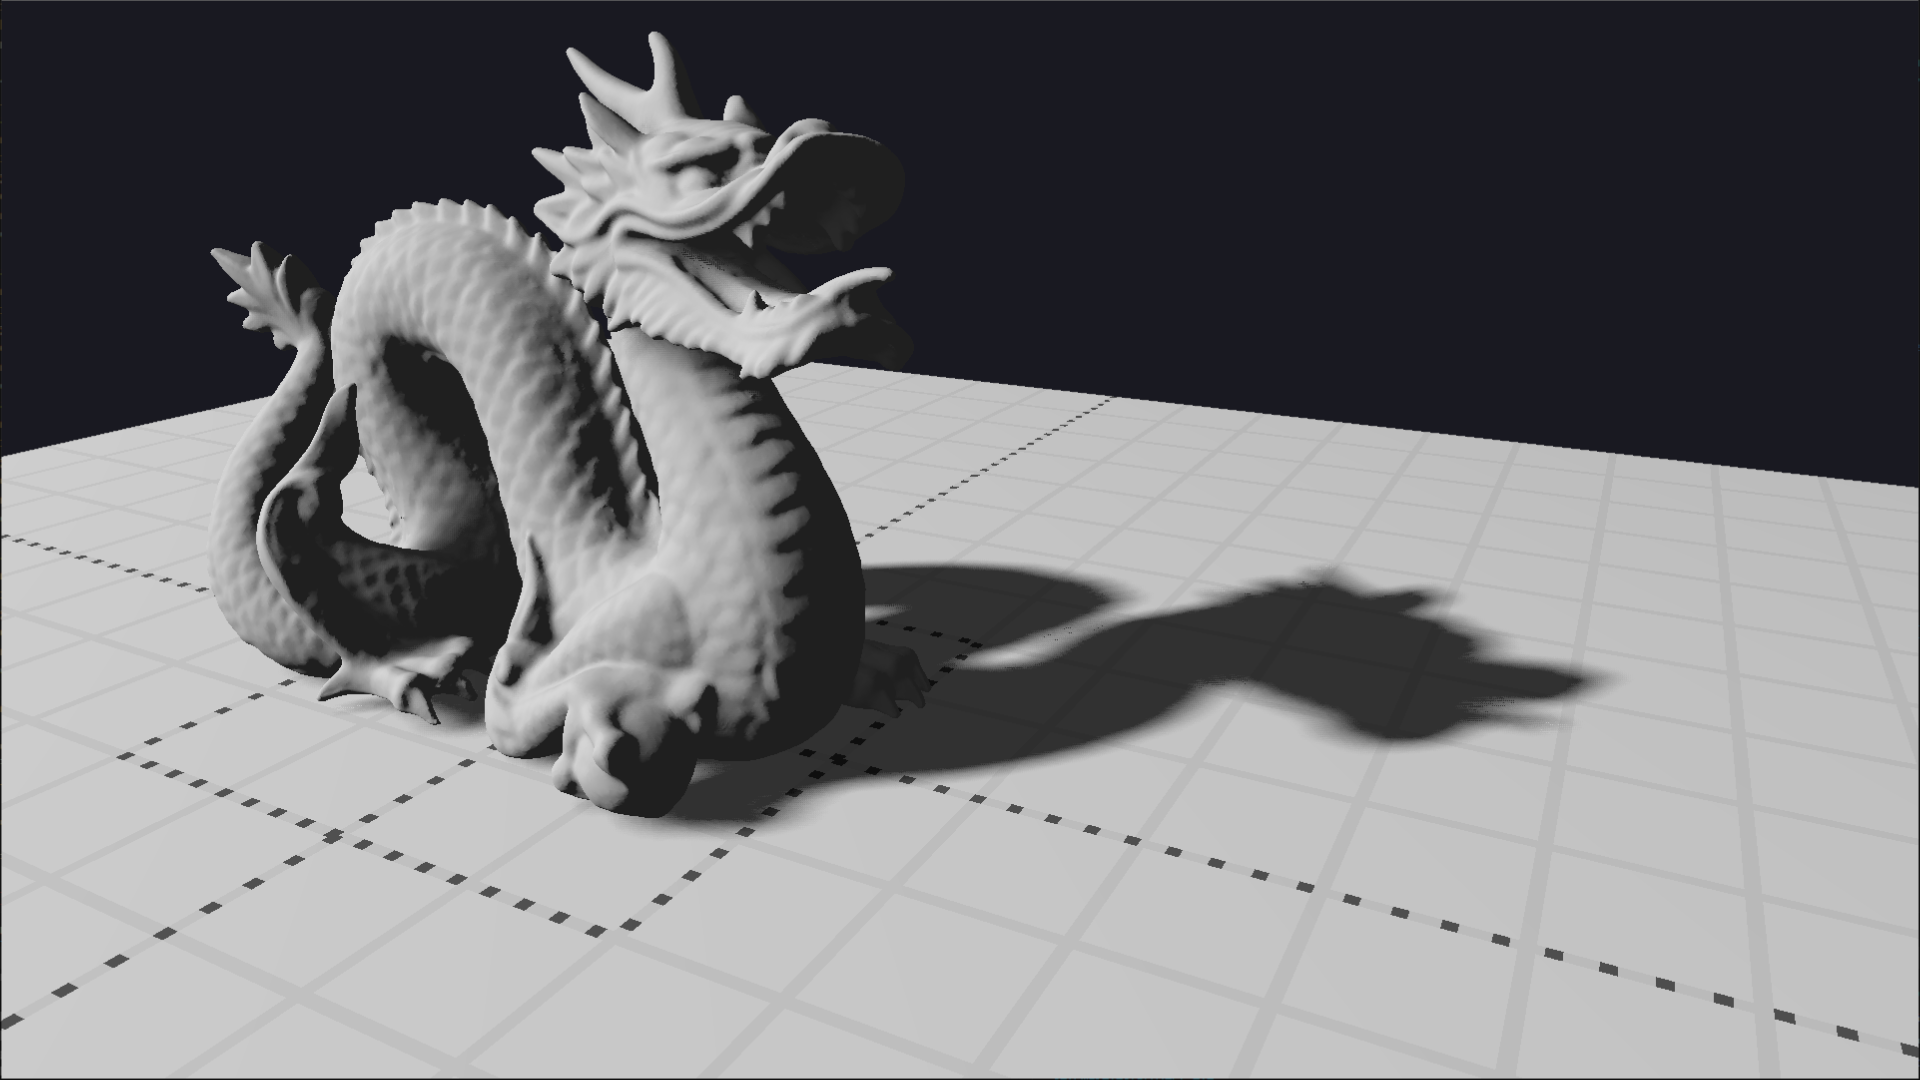
\includegraphics[width=\textwidth]{./graf/tests/adaptive/cropped/dragon_adaptive_fhd_1024_2x2_8x8_offset5.png}
        \caption{The \textit{Chinese Dragon} rendered with \(2\times 2\) set of kernels with adaptive PCF.}
    \end{subfigure}
	\hfill
    \begin{subfigure}[t]{0.45\textwidth}
		\centering
        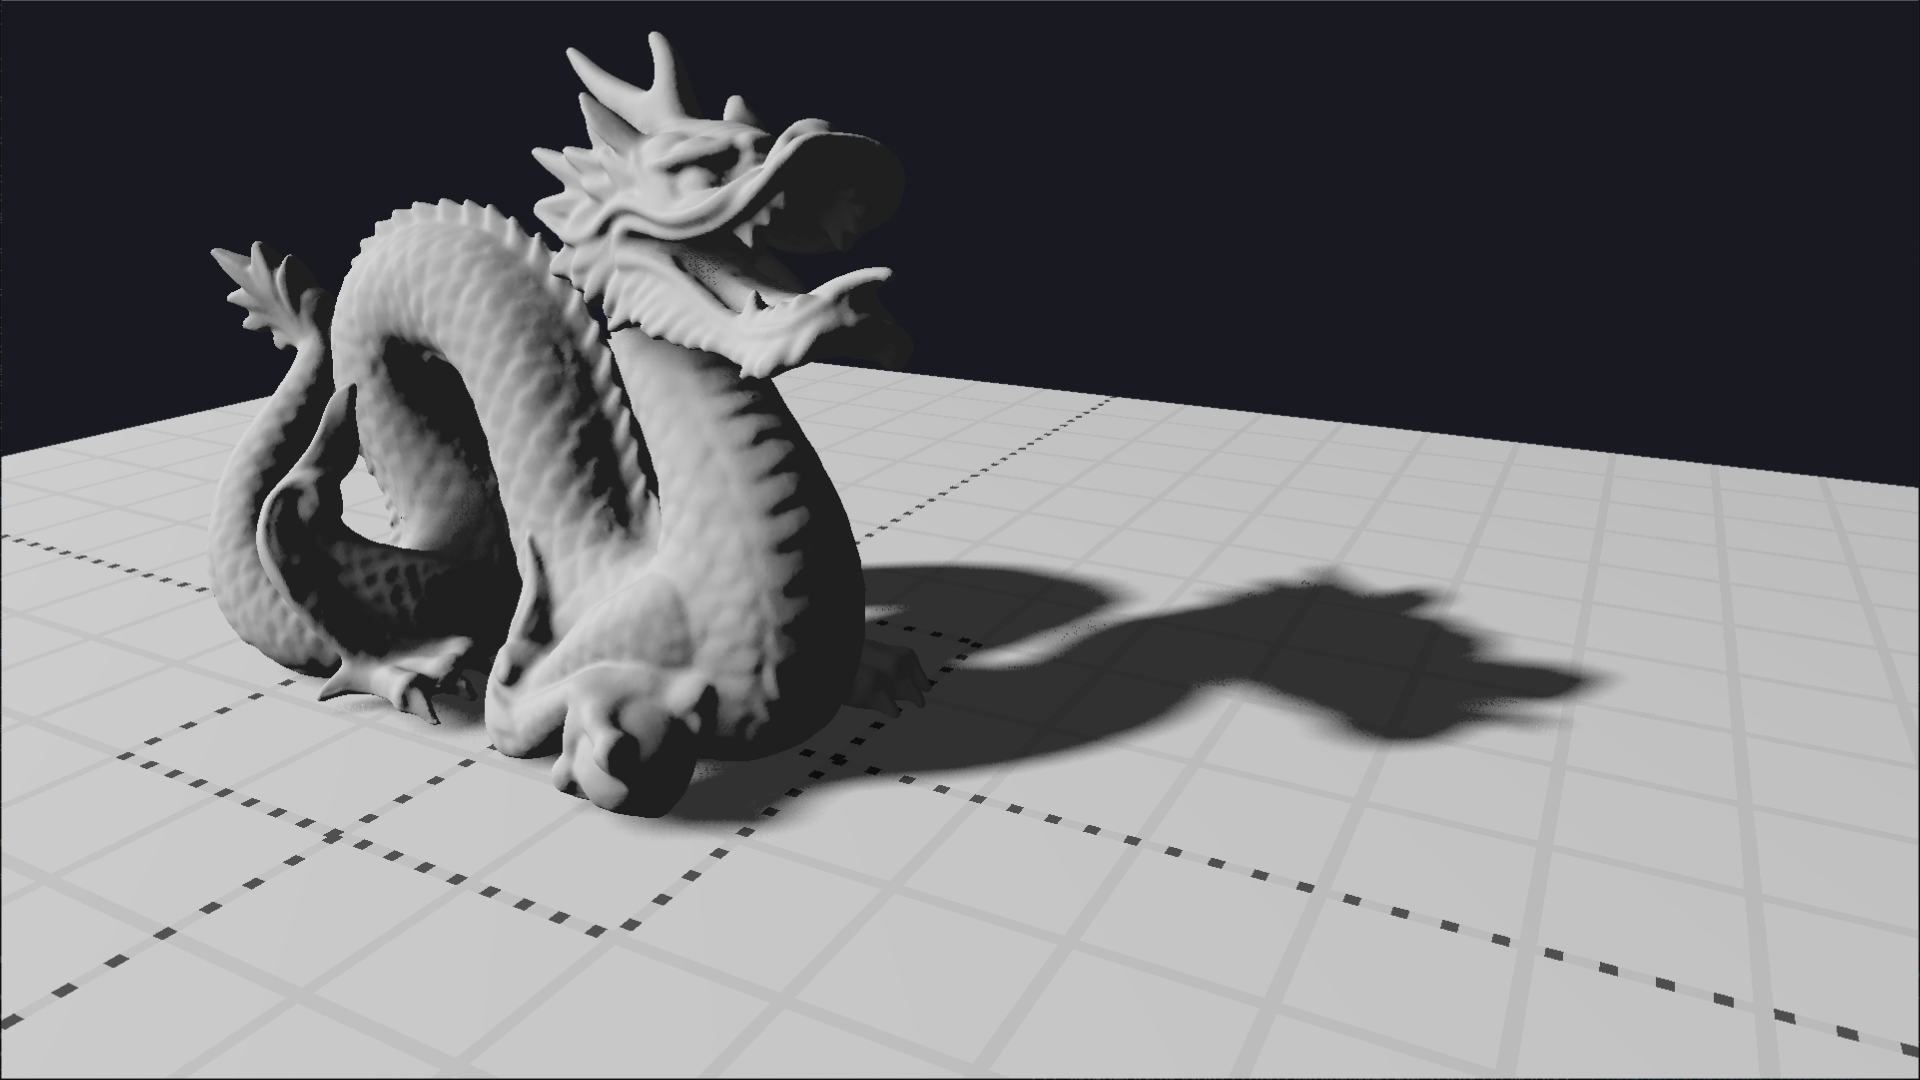
\includegraphics[width=\textwidth]{./graf/tests/adaptive/cropped/dragon_adaptive_fhd_1024_6x6_8x8_offset5.png}
        \caption{The \textit{Chinese Dragon} rendered with \(6\times 6\) set of kernels with adaptive PCF.}
    \end{subfigure}
    \begin{subfigure}[t]{0.45\textwidth}
		\centering
        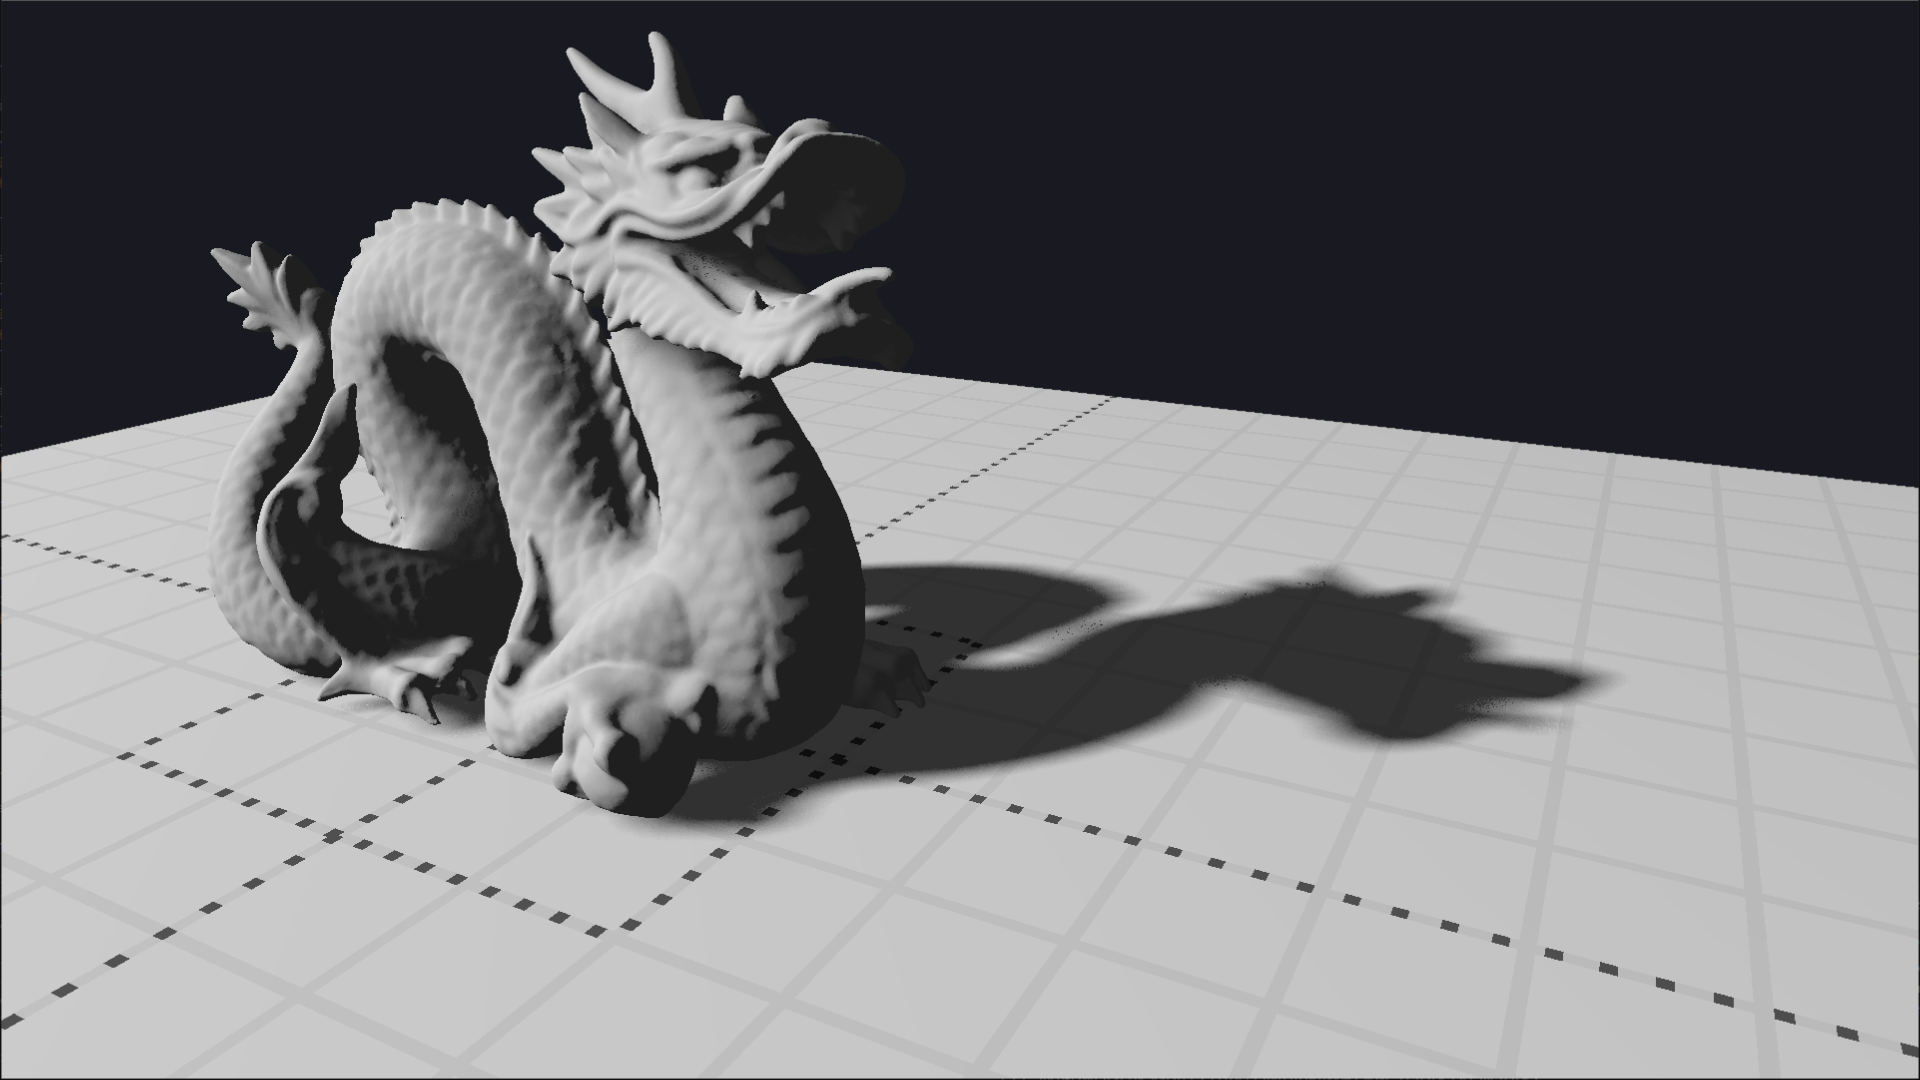
\includegraphics[width=\textwidth]{./graf/tests/adaptive/cropped/dragon_adaptive_fhd_1024_14x14_8x8_offset5.png}
        \caption{The \textit{Chinese Dragon} rendered with \(14\times 14\) set of kernels with adaptive PCF.}
    \end{subfigure}
	\hfill
    \begin{subfigure}[t]{0.45\textwidth}
		\centering
        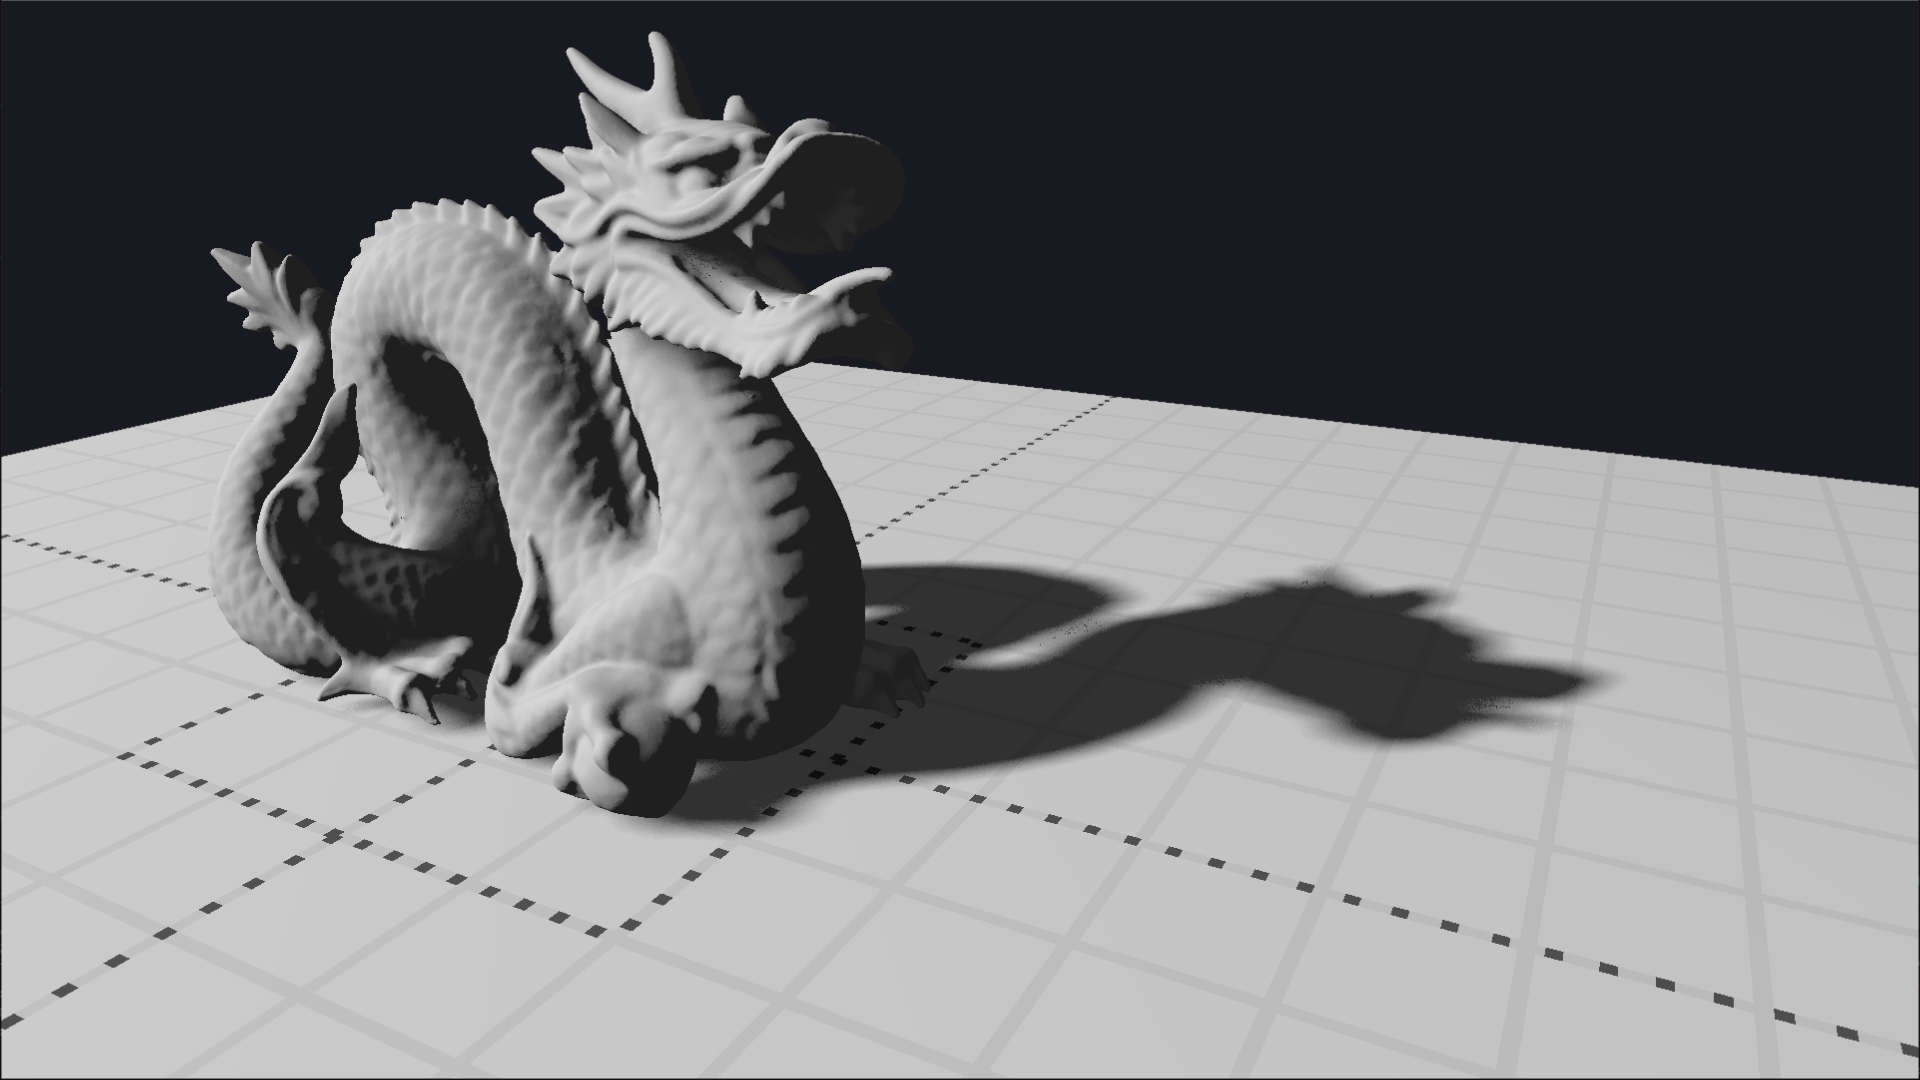
\includegraphics[width=\textwidth]{./graf/tests/adaptive/cropped/dragon_adaptive_fhd_1024_24x24_8x8_offset5.png}
        \caption{The \textit{Chinese Dragon} rendered with \(24\times 24\) set of kernels with adaptive PCF.}
    \end{subfigure}

    \caption{The \textit{Chinese Dragon} rendered with adaptive PCF, using a \(1024\times 1024\) shadow map resolution, kernel size of \(8\times 8\), kernel offset scale of \(5\) and varying counts of kernel sets.}
    \label{fig:test_adaptive_sets_dragon_screens}
\end{figure}

Testing shows no real performance cost of increasing the filter sets count in this range. The kernels are stored in a 3D texture of dimensions \(m\times m \times (n^2/2) \), which is itself generated once on application startup on the CPU, so the cost of generating a large set does not affect FPS. Additionally, accessing a set is simple and efficient, as each output fragment coordinate is simply divided by \(m\) to sample the 3D texture. The sampler is set to wrap the UV addresses, so the filter sets repeat in each direction on screen every \(m\) pixels.

The effect of kernel set count on the visuals is small. For the smallest \(2\times 2\) set there is visible repetition in the structure of the penumbra in the mouth of the dragon or in the shadow near its head. Higher counts provide improvements to the apparent smoothness of the shadow. The difference is a bit more noticeable in movement, where too few sets cause visible repeating patterns in the penumbra regions, that are overlaid on the shadow effect. These artifacts tend to disappear at sizes higher than \(14\times 14\).

As it was mentioned, the 3D texture used to store the kernel offsets has dimensions \(m\times m \times n^2/2\). This means that memory requirements of this technique grow exponentially both with the dimension \(m\) and \(n\). The size is slightly reduced by using a texture with four, \(32\)-bit channels, and storing each \(xy\) offset into two of the channels. This means that two kernel offsets can be stored in a single texel of the texture.

It is worth noting a caveat of this technique that is visible in the results in Fig. \ref{fig:test_adaptive_sets_dragon_screens}. High contrast noise appears in lit areas that are surrounded by shadow, such as in between the neck and back of the dragon's shadow. These erroneous areas stem from the optimization technique. Since the samples farthest away from the kernel center determine if the point is in shadow or not, such areas can get incorrectly classified as shadowed. This issue could be alleviated by using weights when averaging the filter samples, that decrease with the distance from the kernel center.

Overall, the performance and visual results of adaptive PCF make it a very practical solution to filtering shadow maps. The shadows look smooth, and their penumbras are easily controlled with the offset scale.

\subsubsection{Variance shadow maps}
Variance shadow maps were implemented with a separable box filter for blurring of shadows, as explained in section \ref{section:impl_vsm}. This is expected to bring significant performance improvements in comparison to PCF. Below, in Fig. \ref{fig:plot:vsm_results}, are the results of experiments with all the test scenes with different sizes of the filter kernel and for different output resolutions.

\begin{figure}[h]
    \centering
    \begin{subfigure}[t]{0.48\textwidth}
        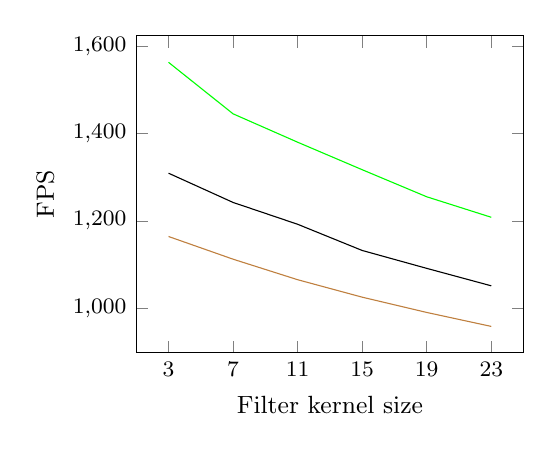
\begin{tikzpicture}
            \begin{axis}[
                small,
                xlabel={Filter kernel size},
                ylabel={FPS},
                xtick={3,7,11,15,19,23},
                xticklabels={3,7,11,15,19,23},
                % legend style={
                %     overlay,
                %     at={(1.25,0.5)},
                %     anchor=center},
                y tick label style={
                    /pgf/number format/.cd,
                        fixed,   % po zakomentowaniu os rzednych jest indeksowana wykladniczo
                        fixed, % 1.0 zamiast 1
                        precision=1,
                    /tikz/.cd
                },
                x tick label style={
                    /pgf/number format/.cd,
                        fixed,
                        fixed,
                        precision=2,
                    /tikz/.cd
                }
                ]
                \addplot [color=green]
                coordinates {
                    (3,1563)(7,1445)(11,1380)(15,1317)(19,1255)(23,1208)}; %\addlegendentry{720p}
                \addplot [color=black]
                coordinates {
                    (3,1309)(7,1242)(11,1192)(15,1132)(19,1091)(23,1051)}; %\addlegendentry{1080p}
                \addplot [color=brown]
                coordinates {
                    (3,1164)(7,1112)(11,1065)(15,1025)(19,990)(23,958)}; %\addlegendentry{2k}
            \end{axis} 
        \end{tikzpicture}
        \caption{Results for the \textit{Chinese Dragon} scene.}
        \label{fig:plot:vsm_dragon}
    \end{subfigure}
    \hfill
    \begin{subfigure}[t]{0.48\textwidth}
        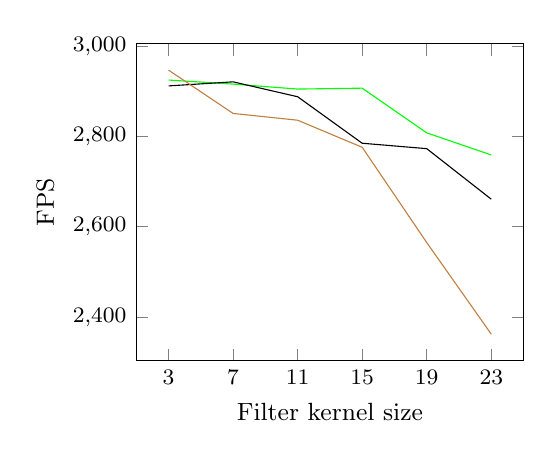
\begin{tikzpicture}
            \begin{axis}[
                small,
                xlabel={Filter kernel size},
                ylabel={FPS},
                xtick={3,7,11,15,19,23},
                xticklabels={3,7,11,15,19,23},
                % legend style={
                %     overlay,
                %     at={(1.25,0.5)},
                %     anchor=center},
                y tick label style={
                    /pgf/number format/.cd,
                        fixed,   % po zakomentowaniu os rzednych jest indeksowana wykladniczo
                        fixed, % 1.0 zamiast 1
                        precision=1,
                    /tikz/.cd
                },
                x tick label style={
                    /pgf/number format/.cd,
                        fixed,
                        fixed,
                        precision=2,
                    /tikz/.cd
                }
                ]
                \addplot [color=green]
                coordinates {
                    (3,2925)(7,2916)(11,2905)(15,2907)(19,2808)(23,2759)}; %\addlegendentry{720p}
                \addplot [color=black]
                coordinates {
                    (3,2912)(7,2921)(11,2888)(15,2785)(19,2773)(23,2661)}; %\addlegendentry{1080p}
                \addplot [color=brown]
                coordinates {
                    (3,2947)(7,2851)(11,2836)(15,2776)(19,2565)(23,2362)}; %\addlegendentry{2k}
            \end{axis} 
        \end{tikzpicture}
        \caption{Results for the \textit{Cube} scene.}
        \label{fig:plot:vsm_cube}
    \end{subfigure}

    \vspace{20pt}
    \begin{subfigure}[t]{0.48\textwidth}
        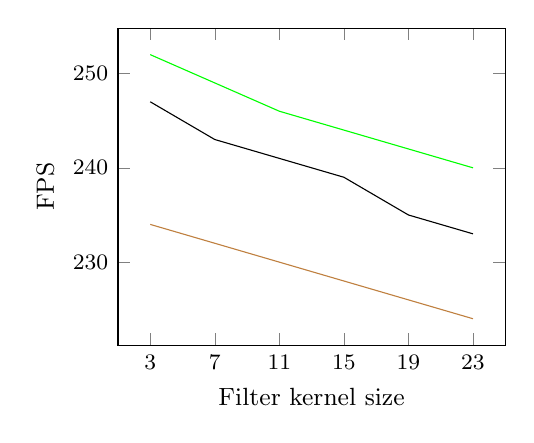
\begin{tikzpicture}
            \begin{axis}[
                small,
                xlabel={Filter kernel size},
                ylabel={FPS},
                xtick={3,7,11,15,19,23},
                xticklabels={3,7,11,15,19,23},
                % legend style={
                %     overlay,
                %     at={(1.25,0.5)},
                %     anchor=center},
                y tick label style={
                    /pgf/number format/.cd,
                        fixed,   % po zakomentowaniu os rzednych jest indeksowana wykladniczo
                        fixed, % 1.0 zamiast 1
                        precision=1,
                    /tikz/.cd
                },
                x tick label style={
                    /pgf/number format/.cd,
                        fixed,
                        fixed,
                        precision=2,
                    /tikz/.cd
                }
                ]
                \addplot [color=green]
                coordinates {
                    (3,252)(7,249)(11,246)(15,244)(19,242)(23,240)}; %\addlegendentry{720p}
                \addplot [color=black]
                coordinates {
                    (3,247)(7,243)(11,241)(15,239)(19,235)(23,233)}; %\addlegendentry{1080p}
                \addplot [color=brown]
                coordinates {
                    (3,234)(7,232)(11,230)(15,228)(19,226)(23,224)}; %\addlegendentry{2k}
            \end{axis} 
        \end{tikzpicture}
        \caption{Results for the \textit{Power Plant} scene.}
        \label{fig:plot:vsm_power}
    \end{subfigure}
    \hfill
    \begin{subfigure}[t]{0.48\textwidth}
        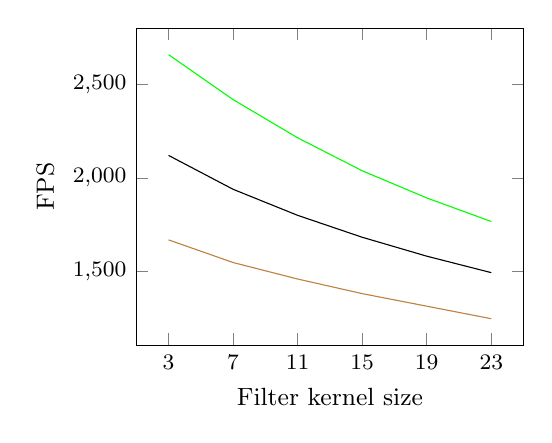
\begin{tikzpicture}
            \begin{axis}[
                small,
                xlabel={Filter kernel size},
                ylabel={FPS},
                xtick={3,7,11,15,19,23},
                xticklabels={3,7,11,15,19,23},
                % legend style={
                %     overlay,
                %     at={(1.25,0.5)},
                %     anchor=center},
                y tick label style={
                    /pgf/number format/.cd,
                        fixed,   % po zakomentowaniu os rzednych jest indeksowana wykladniczo
                        fixed, % 1.0 zamiast 1
                        precision=1,
                    /tikz/.cd
                },
                x tick label style={
                    /pgf/number format/.cd,
                        fixed,
                        fixed,
                        precision=2,
                    /tikz/.cd
                }
                ]
                \addplot [color=green]
                coordinates {
                    (3,2658)(7,2418)(11,2214)(15,2038)(19,1893)(23,1767)}; %\addlegendentry{720p}
                \addplot [color=black]
                coordinates {
                    (3,2120)(7,1939)(11,1800)(15,1683)(19,1582)(23,1494)}; %\addlegendentry{1080p}
                \addplot [color=brown]
                coordinates {
                    (3,1669)(7,1548)(11,1460)(15,1382)(19,1315)(23,1248)}; %\addlegendentry{2k}
            \end{axis} 
        \end{tikzpicture}
        \caption{Results for the \textit{Crytek Sponza} scene.}
        \label{fig:plot:vsm_sponza}
    \end{subfigure}
    \caption{Frames per second for all test scenes, for different sizes of the filter kernel and output resolutions. In green \(1280\times 720\), in black \(1920\times 1080\) and in brown \(2560\times 1440\). Rendering with the variance shadow mapping technique with box filtering, at constant shadow map size \(1024\times 1024\).}
    \label{fig:plot:vsm_results}
\end{figure}

The results are exceptionally good, showing performance much better than PCF and even adaptive PCF. The tests were performed with twice as large filter kernels as in the case of PCF and FPS never dropped below 224 in the worst case. The performance degradation, if extrapolated from these plots, also seems to be slowing down, which hints that even larger kernel sizes are within reach with this technique.

During testing comparisons of regular shadow mapping and VSM without any filtering were performed, and VSM usually scored just up to 5 FPS worse. If it is intended to be used with any kind of filtering, then this cost of the pure VSM algorithm is well worth it.

Variance shadow maps introduce higher memory requirements which has to be taken into account when working with particularly restrictive memory budgets. VSM in itself requires a texture with two-channels, each 32-bit to avoid numeric issues. In addition, a separate depth buffer has to be used, which adds another 32-bit resource. This is three times the memory consumption of a basic shadow mapping implementation. If filtering is to be utilized, another resource of same size and format as the VSM is needed to perform separable filtering.

Visually, VSM is very good at anti-aliasing and smoothing shadows. Large filter kernels can be used with great performance. When combined with standard bilinear texture filtering the results are perfectly smooth. Unfortunately this technique tends to lose detail in the shadows. It also suffers from light leaks that need to be tweaked by hand to disappear and artifacts can occur in places where occluders overlap. On the other hand it is mostly free of shadow acne, even at highest filter sizes. Results of rendering with VSM, including its pitfalls, are presented in Fig. \ref{fig:test_vsm_screens}.

\begin{figure}[h]
    \centering
    \begin{subfigure}[t]{0.49\textwidth}
		\centering
        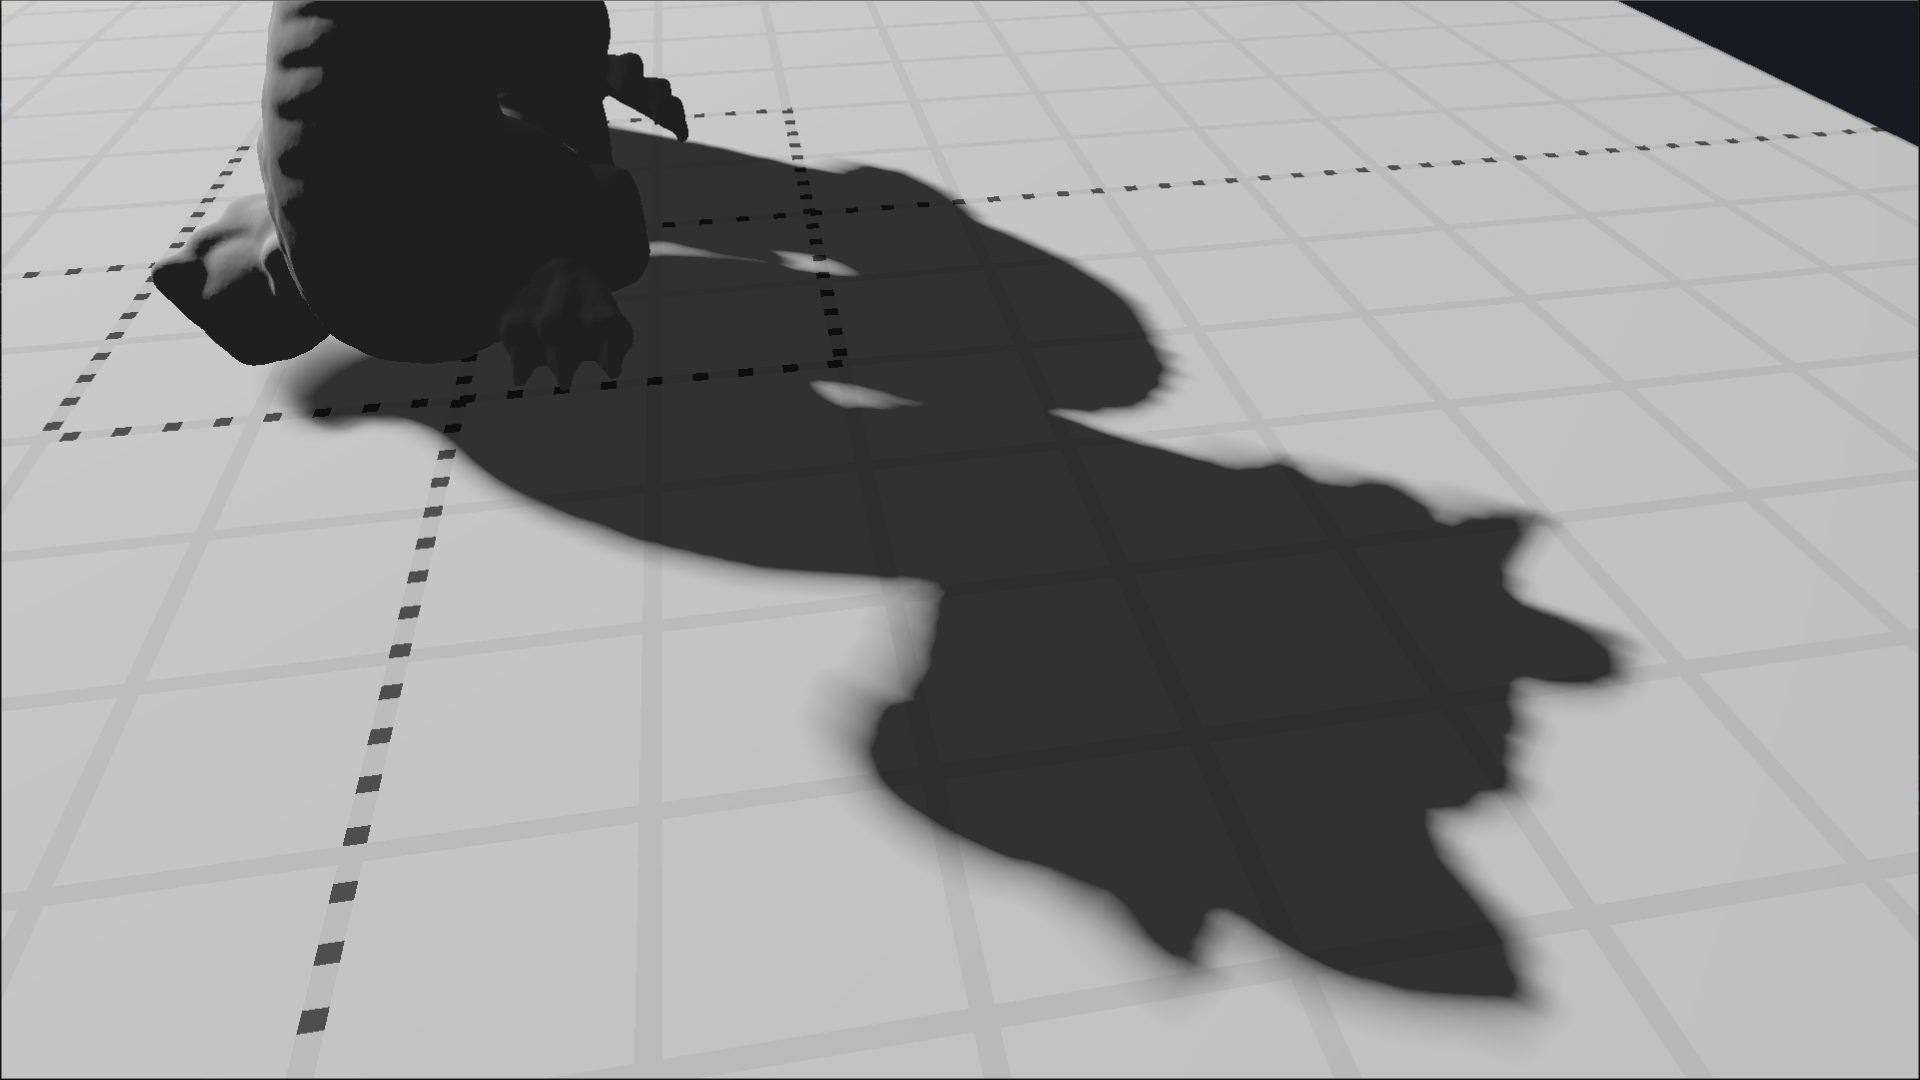
\includegraphics[width=\textwidth]{./graf/tests/vsm/cropped/dragon_vsm_512_23_smooth.png}
        \caption{The \textit{Chinese Dragon} rendered with \(11\times 11\) kernel with bilinear filtering and low resolution \(512\times 512\) shadow map. The shadow is very smooth, but has lost some detail.}
    \end{subfigure}
	\hfill
    \begin{subfigure}[t]{0.49\textwidth}
		\centering
        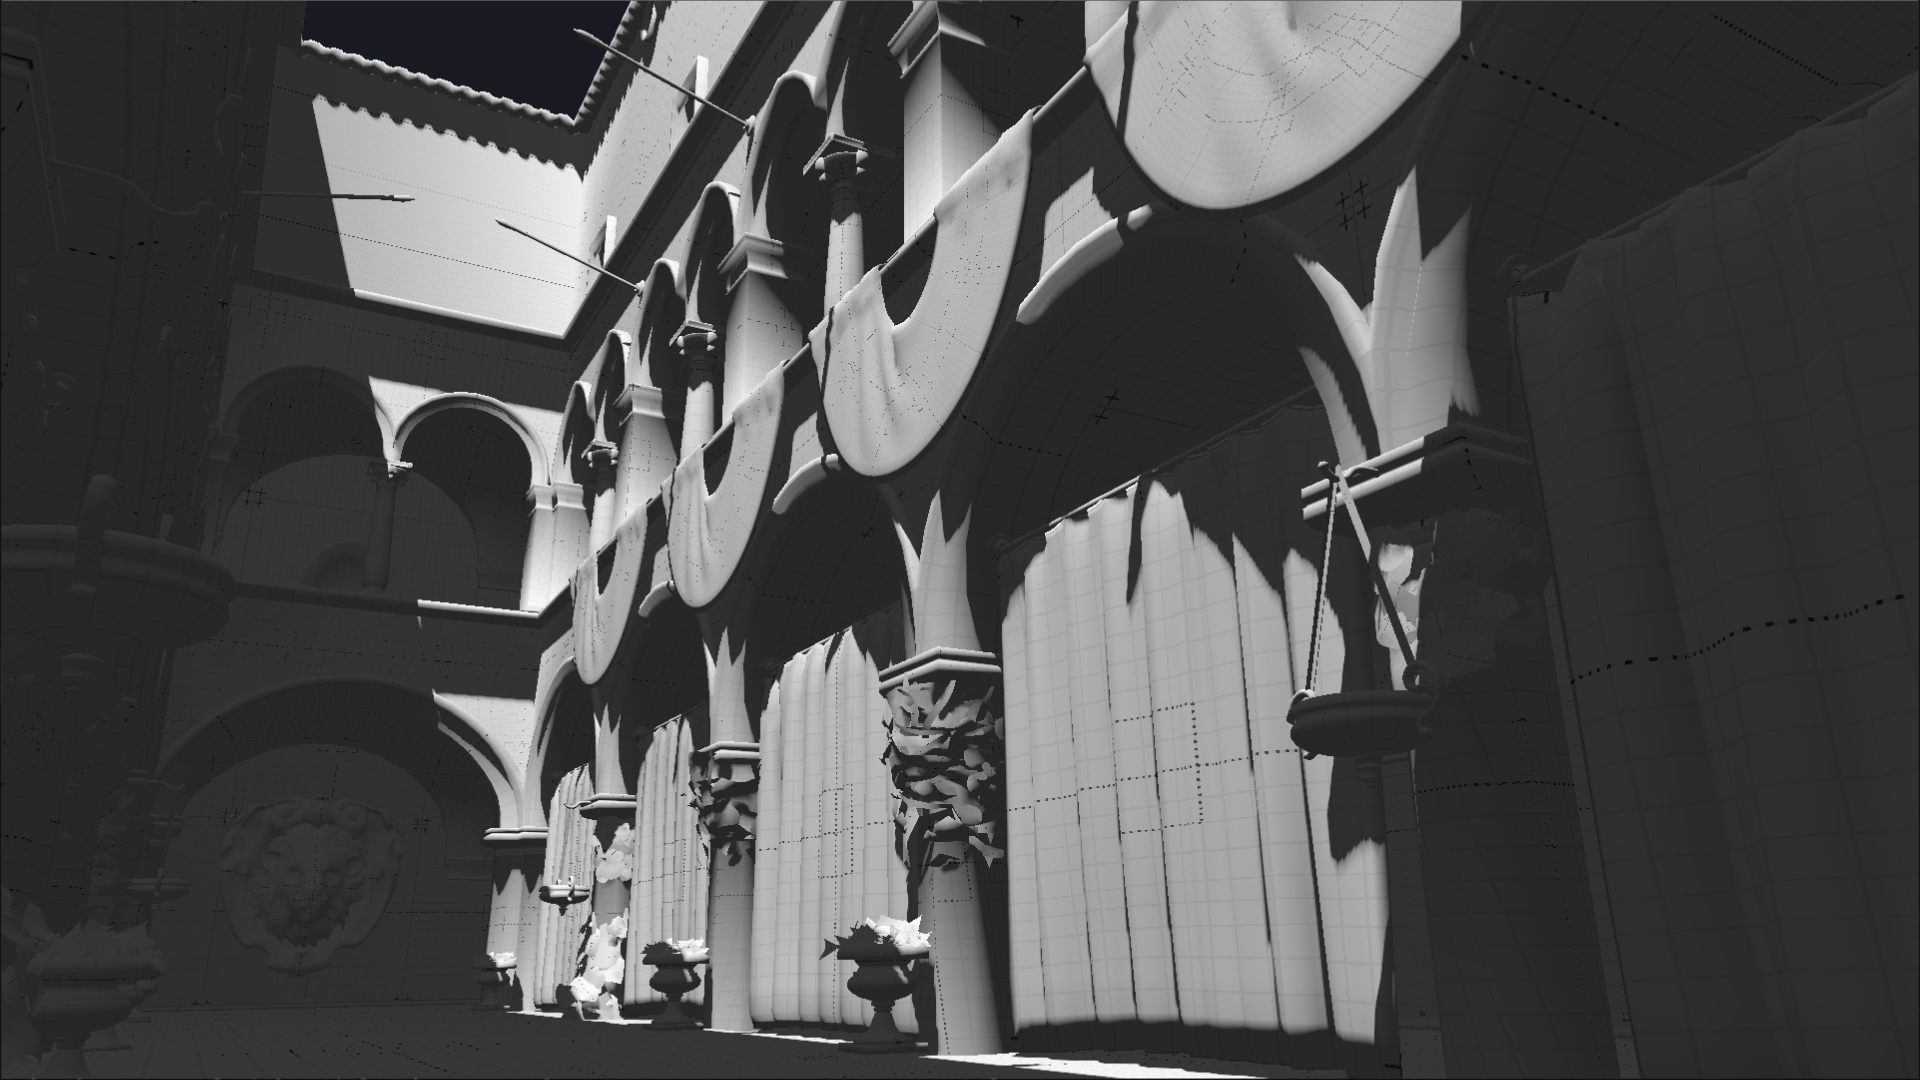
\includegraphics[width=\textwidth]{./graf/tests/vsm/cropped/sponza_vsm_4096_23.png}
        \caption{The \textit{Crytek Sponza} scene rendered with VSM producing very pleasant shadows.}
    \end{subfigure}
    \begin{subfigure}[t]{0.49\textwidth}
		\centering
        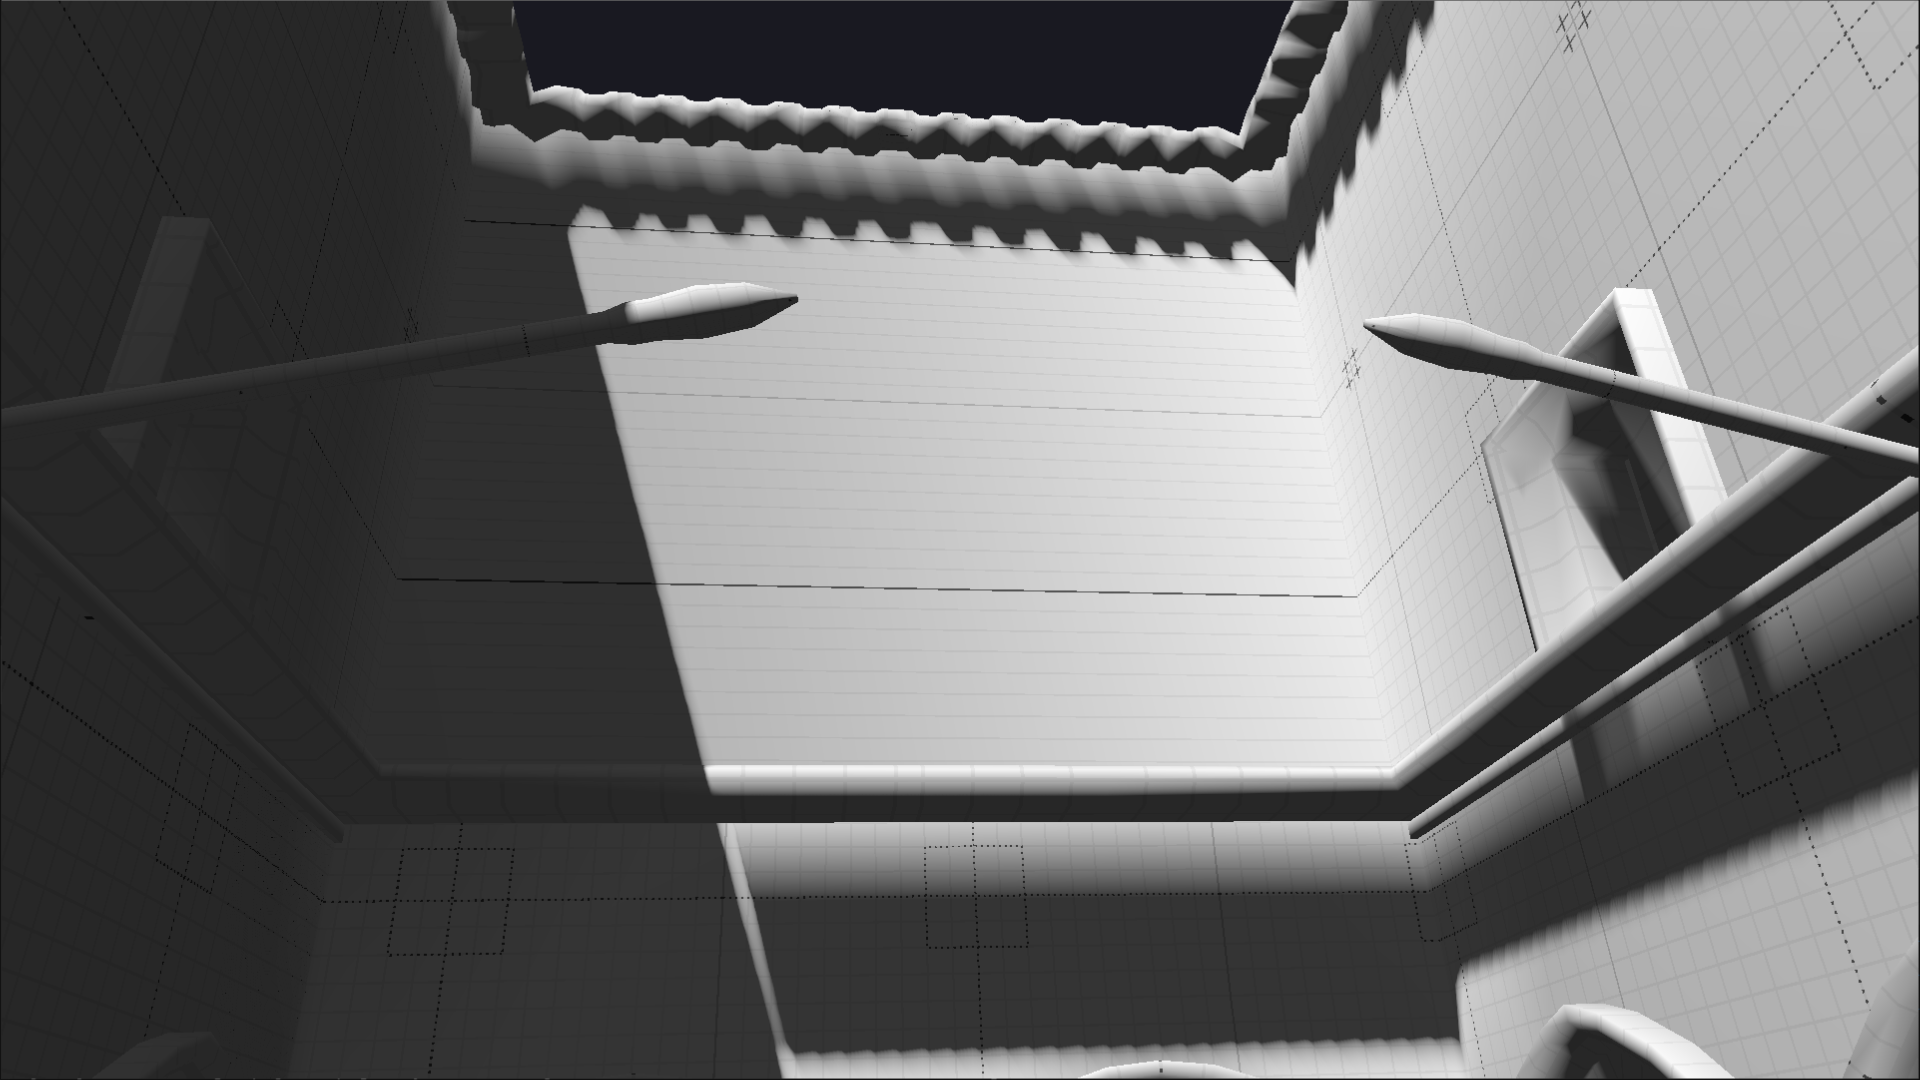
\includegraphics[width=\textwidth]{./graf/tests/vsm/cropped/sponza_vsm_4096_23_badsetup.png}
        \caption{The \textit{Crytek Sponza} scene rendered with VSM exhibiting light leaking due to wrong selection of parameters.}
    \end{subfigure}
	\hfill
    \begin{subfigure}[t]{0.49\textwidth}
		\centering
        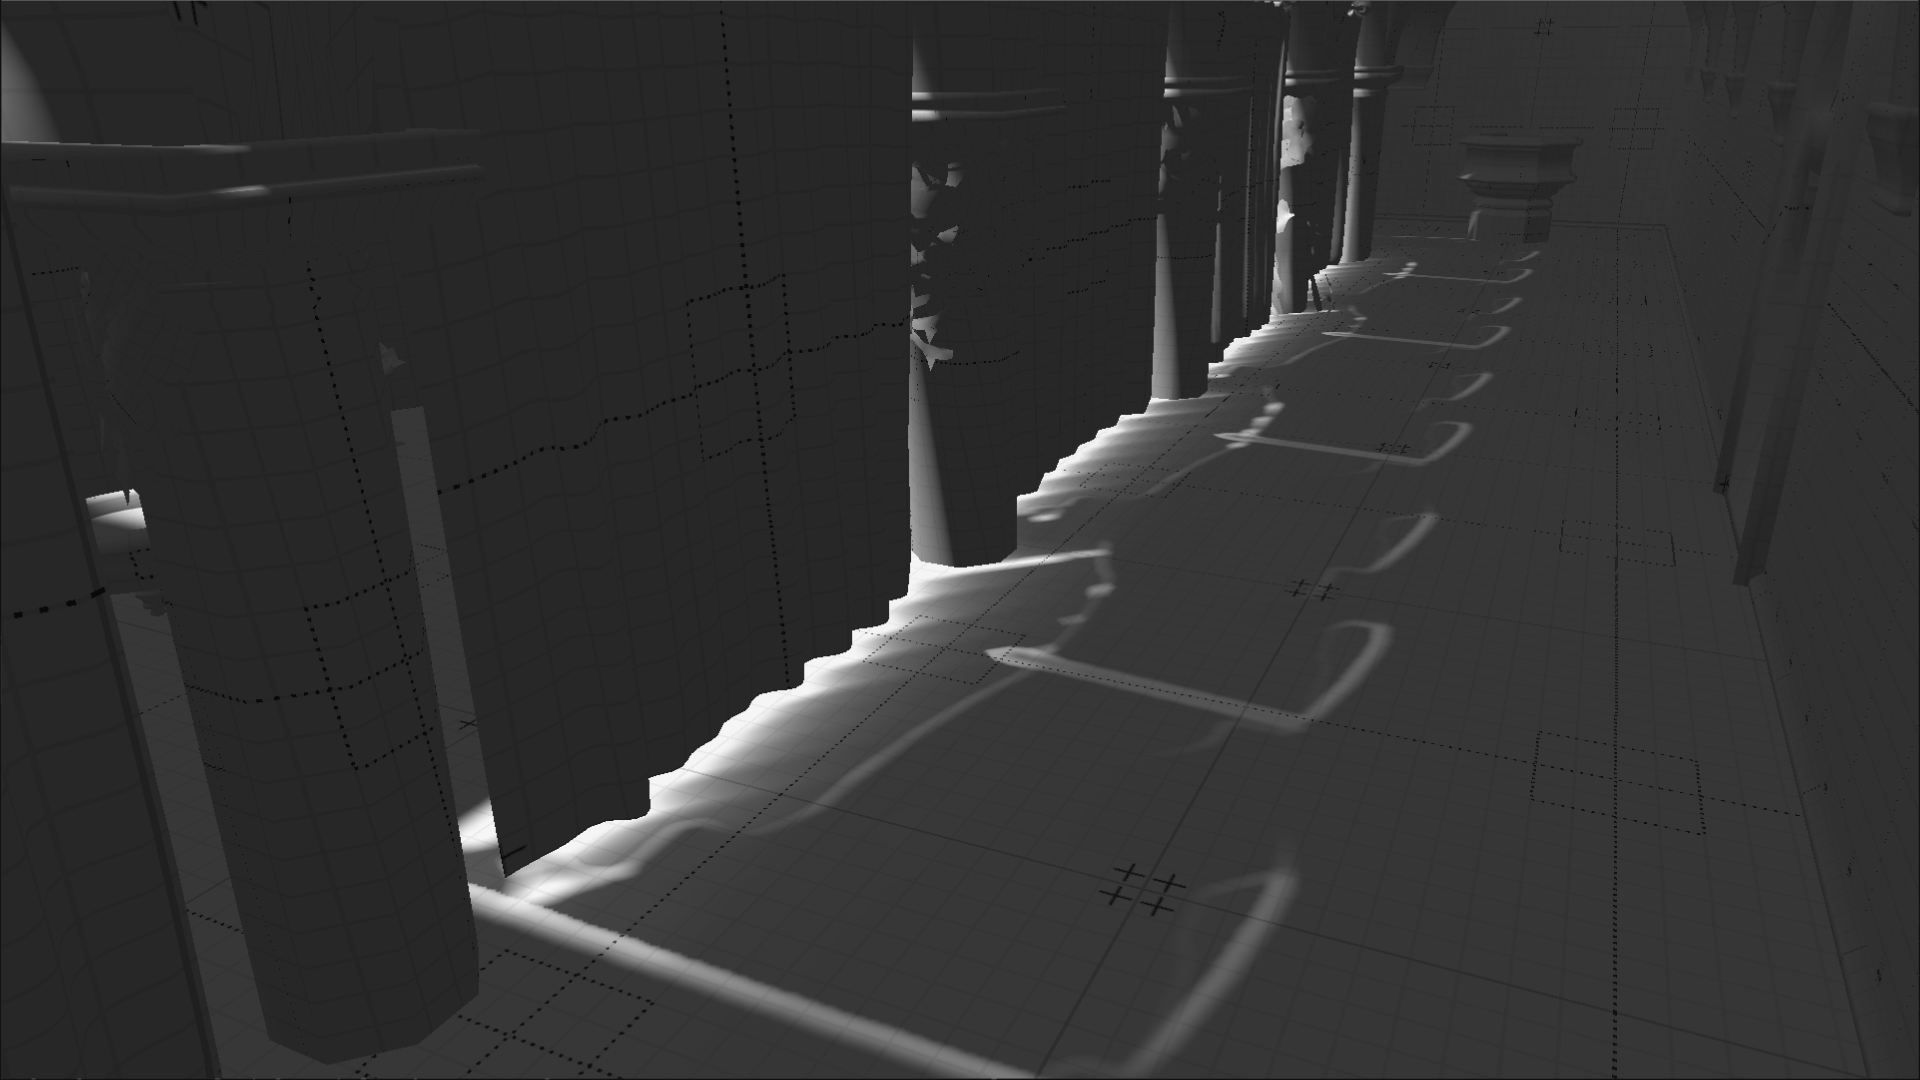
\includegraphics[width=\textwidth]{./graf/tests/vsm/cropped/sponza_vsm_4096_23_leaks.png}
        \caption{The \textit{Crytek Sponza} scene rendered with VSM with visible light leaks due to incorrect parameters.}
    \end{subfigure}

    \caption{Test scenes showcasing pros and cons of VSM.}
    \label{fig:test_vsm_screens}
\end{figure}

\subsection{Soft shadows with shadow maps}

\subsubsection{PCSS}
Implementation of percentage-closer soft shadows was presented in section \ref{section:pcss}. This section presents the results of testing this technique. Figure \ref{fig:plot:pcss_results} shows FPS measurements for all test scenes with different light source sizes, which define the size of the penumbra and impact overall performance. PCSS is implemented here using adaptive techniques for both finding the average occluder depth and filtering.

\begin{figure}[h]
    \centering
    \begin{subfigure}[t]{0.48\textwidth}
        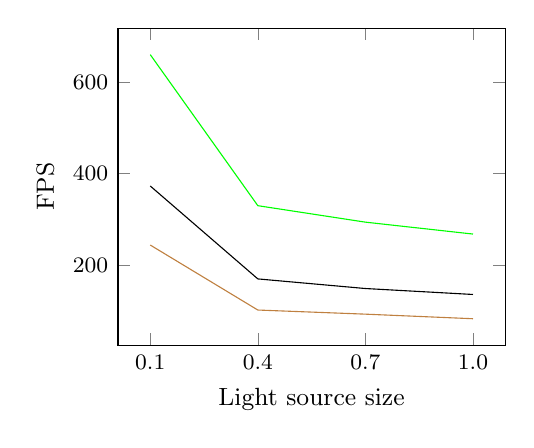
\begin{tikzpicture}
            \begin{axis}[
                small,
                xlabel={Light source size},
                ylabel={FPS},
                xtick={0.1,0.4,0.7,1.0},
                xticklabels={0.1,0.4,0.7,1.0},
                % legend style={
                %     overlay,
                %     at={(1.25,0.5)},
                %     anchor=center},
                y tick label style={
                    /pgf/number format/.cd,
                        fixed,   % po zakomentowaniu os rzednych jest indeksowana wykladniczo
                        fixed, % 1.0 zamiast 1
                        precision=1,
                    /tikz/.cd
                },
                x tick label style={
                    /pgf/number format/.cd,
                        fixed,
                        fixed,
                        precision=2,
                    /tikz/.cd
                }
                ]
                \addplot [color=green]
                coordinates {
                    (0.1,660)(0.4,330)(0.7,294)(1.0,268)}; %\addlegendentry{720p}
                \addplot [color=black]
                coordinates {
                    (0.1,373)(0.4,170)(0.7,149)(1.0,136)}; %\addlegendentry{1080p}
                \addplot [color=brown]
                coordinates {
                    (0.1,244)(0.4,102)(0.7,93)(1.0,83)}; %\addlegendentry{2k}
            \end{axis} 
        \end{tikzpicture}
        \caption{Results for the \textit{Chinese Dragon} scene.}
        \label{fig:plot:pcss_dragon}
    \end{subfigure}
    \hfill
    \begin{subfigure}[t]{0.48\textwidth}
        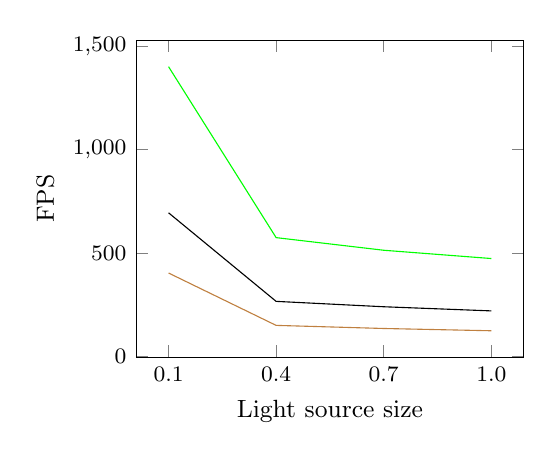
\begin{tikzpicture}
            \begin{axis}[
                small,
                xlabel={Light source size},
                ylabel={FPS},
                xtick={0.1,0.4,0.7,1.0},
                xticklabels={0.1,0.4,0.7,1.0},
                % legend style={
                %     overlay,
                %     at={(1.25,0.5)},
                %     anchor=center},
                y tick label style={
                    /pgf/number format/.cd,
                        fixed,   % po zakomentowaniu os rzednych jest indeksowana wykladniczo
                        fixed, % 1.0 zamiast 1
                        precision=1,
                    /tikz/.cd
                },
                x tick label style={
                    /pgf/number format/.cd,
                        fixed,
                        fixed,
                        precision=2,
                    /tikz/.cd
                }
                ]
                \addplot [color=green]
                coordinates {
                    (0.1,1401)(0.4,575)(0.7,514)(1.0,474)}; %\addlegendentry{720p}
                \addplot [color=black]
                coordinates {
                    (0.1,695)(0.4,267)(0.7,241)(1.0,221)}; %\addlegendentry{1080p}
                \addplot [color=brown]
                coordinates {
                    (0.1,404)(0.4,151)(0.7,136)(1.0,125)}; %\addlegendentry{2k}
            \end{axis} 
        \end{tikzpicture}
        \caption{Results for the \textit{Cube} scene.}
        \label{fig:plot:pcss_cube}
    \end{subfigure}

    \vspace{20pt}
    \begin{subfigure}[t]{0.48\textwidth}
        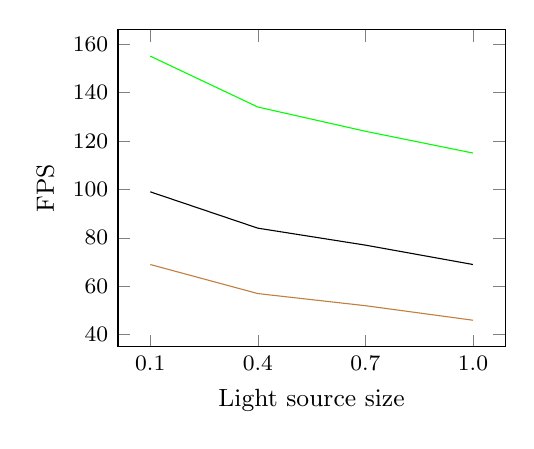
\begin{tikzpicture}
            \begin{axis}[
                small,
                xlabel={Light source size},
                ylabel={FPS},
                xtick={0.1,0.4,0.7,1.0},
                xticklabels={0.1,0.4,0.7,1.0},
                % legend style={
                %     overlay,
                %     at={(1.25,0.5)},
                %     anchor=center},
                y tick label style={
                    /pgf/number format/.cd,
                        fixed,   % po zakomentowaniu os rzednych jest indeksowana wykladniczo
                        fixed, % 1.0 zamiast 1
                        precision=1,
                    /tikz/.cd
                },
                x tick label style={
                    /pgf/number format/.cd,
                        fixed,
                        fixed,
                        precision=2,
                    /tikz/.cd
                }
                ]
                \addplot [color=green]
                coordinates {
                    (0.1,155)(0.4,134)(0.7,124)(1.0,115)}; %\addlegendentry{720p}
                \addplot [color=black]
                coordinates {
                    (0.1,99)(0.4,84)(0.7,77)(1.0,69)}; %\addlegendentry{1080p}
                \addplot [color=brown]
                coordinates {
                    (0.1,69)(0.4,57)(0.7,52)(1.0,46)}; %\addlegendentry{2k}
            \end{axis} 
        \end{tikzpicture}
        \caption{Results for the \textit{Power Plant} scene.}
        \label{fig:plot:pss_power}
    \end{subfigure}
    \hfill
    \begin{subfigure}[t]{0.48\textwidth}
        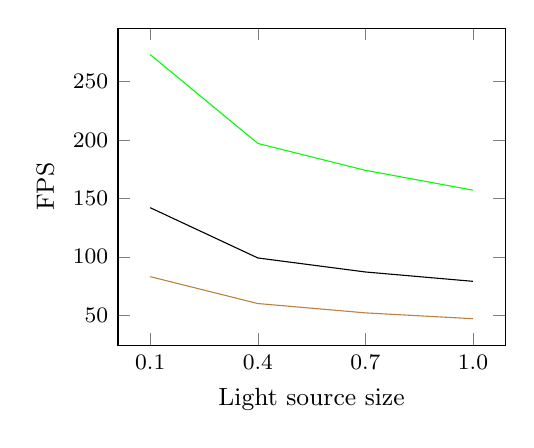
\begin{tikzpicture}
            \begin{axis}[
                small,
                xlabel={Light source size},
                ylabel={FPS},
                xtick={0.1,0.4,0.7,1.0},
                xticklabels={0.1,0.4,0.7,1.0},
                % legend style={
                %     overlay,
                %     at={(1.25,0.5)},
                %     anchor=center},
                y tick label style={
                    /pgf/number format/.cd,
                        fixed,   % po zakomentowaniu os rzednych jest indeksowana wykladniczo
                        fixed, % 1.0 zamiast 1
                        precision=1,
                    /tikz/.cd
                },
                x tick label style={
                    /pgf/number format/.cd,
                        fixed,
                        fixed,
                        precision=2,
                    /tikz/.cd
                }
                ]
                \addplot [color=green]
                coordinates {
                    (0.1,273)(0.4,197)(0.7,174)(1.0,157)}; %\addlegendentry{720p}
                \addplot [color=black]
                coordinates {
                    (0.1,142)(0.4,99)(0.7,87)(1.0,79)}; %\addlegendentry{1080p}
                \addplot [color=brown]
                coordinates {
                    (0.1,83)(0.4,60)(0.7,52)(1.0,47)}; %\addlegendentry{2k}
            \end{axis} 
        \end{tikzpicture}
        \caption{Results for the \textit{Crytek Sponza} scene.}
        \label{fig:plot:pcss_sponza}
    \end{subfigure}
    \caption{Frames per second for all test scenes, for different sizes of the light source and output resolutions. In green \(1280\times 720\), in black \(1920\times 1080\) and in brown \(2560\times 1440\). Rendering with shadow mapping with PCSS at constant shadow map size \(1024\times 1024\) and \(16\times 16\) \(8\times 8\) kernels.}
    \label{fig:plot:pcss_results}
\end{figure}

Performance is affected more negatively than with adaptive PCF. This decrease happens because PCSS basically performs two adaptive filtering-like steps per-pixel. It first has to sample the shadow map to find the average occluder depth and then again for PCF with a calculated size. For simpler scenes however, as the size of the light source increases, there seems to be a threshold value beyond which the performance degradation slows down. This is probably because in the case of a simple scene like the \textit{Chinese Dragon} or the \textit{Cube}, once the light source is large enough almost all surfaces will be evaluated as if in a penumbra. Additionally, very high light source sizes produce unpleasant results and should not be used in a real application anyway.

The light size needs to be carefully tuned on a per-scene basis to get plausible results. Additionally, bias has to be adjusted to account for wider kernels. Images rendered with PCSS are presented in Fig \ref{fig:test_pcss_screens}.
\begin{figure}[h]
    \centering
    \begin{subfigure}[t]{0.49\textwidth}
		\centering
        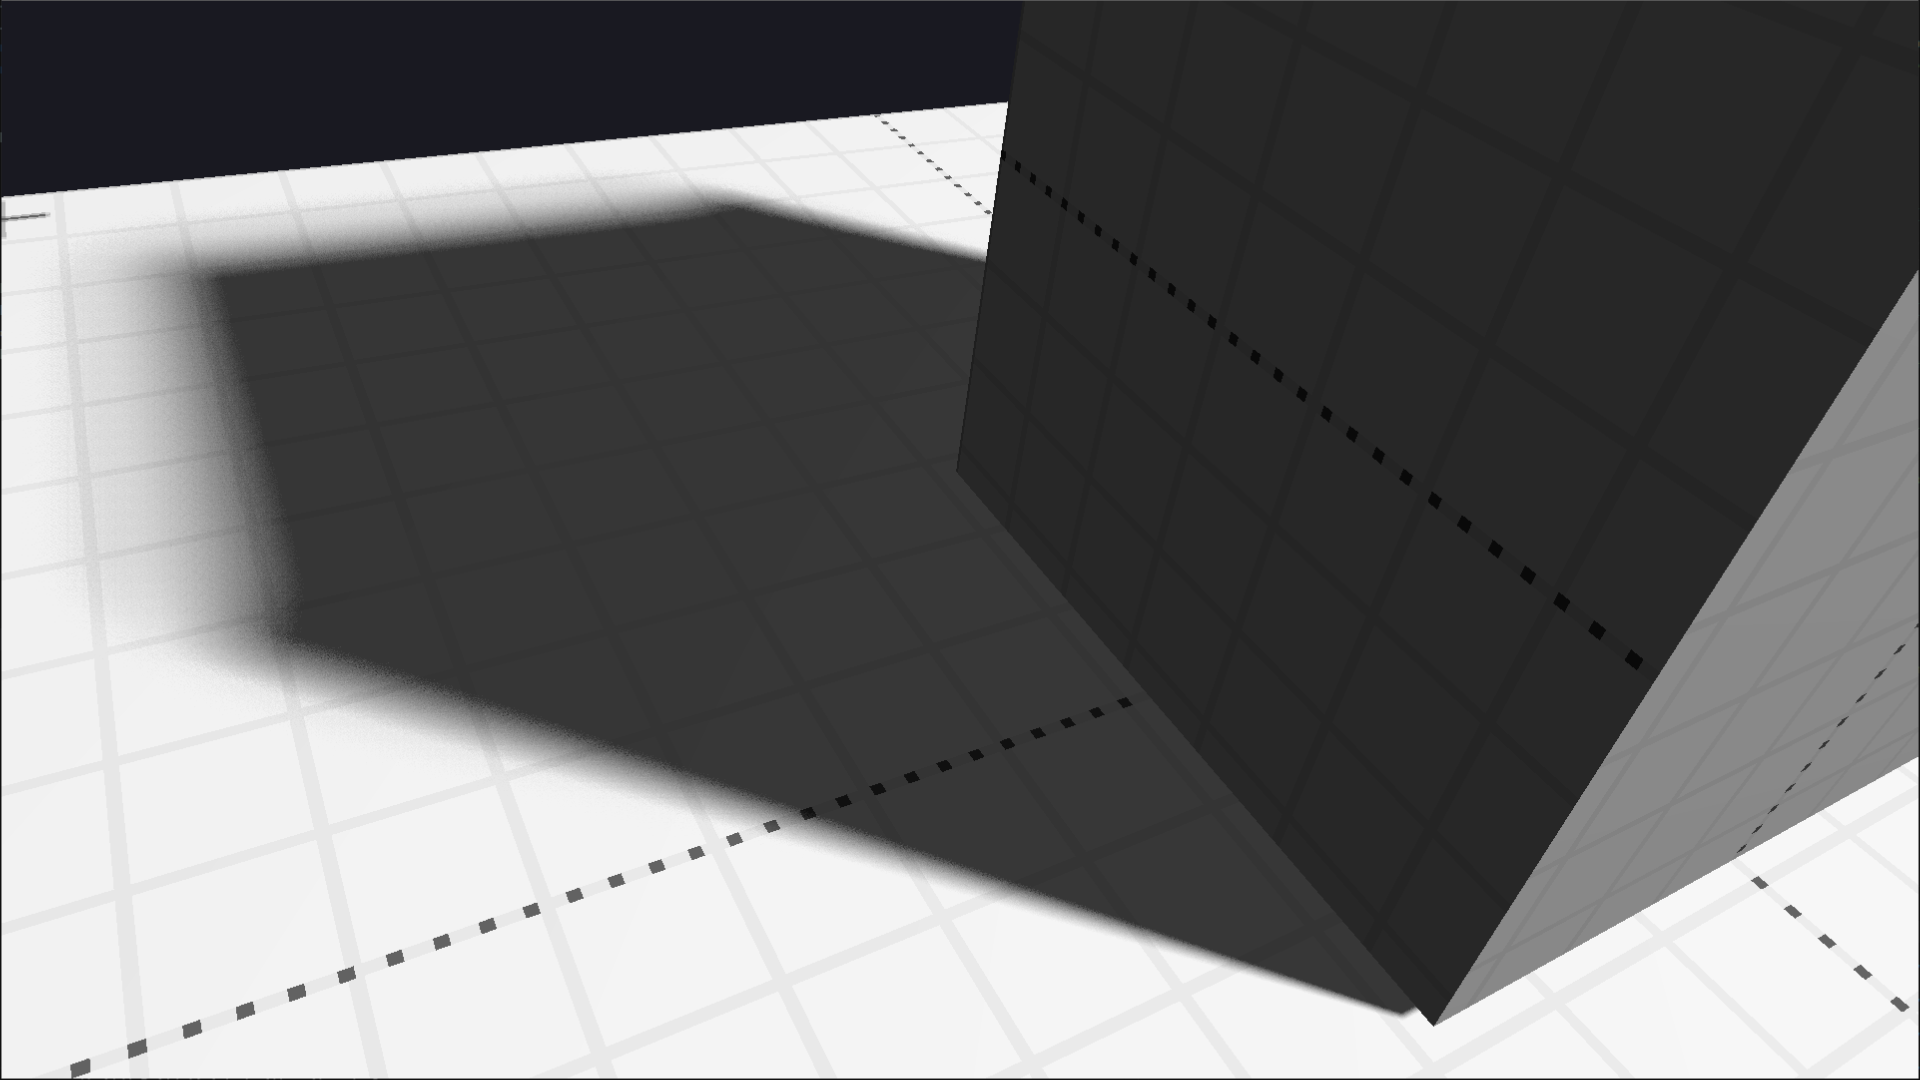
\includegraphics[width=\textwidth]{./graf/tests/pcss/cropped/cube_pcss_1.png}
        \caption{The \textit{Cube} scene showing smooth shadow penumbra falloff with changing distance between shadow caster and receiver.}
    \end{subfigure}
	\hfill
    \begin{subfigure}[t]{0.49\textwidth}
		\centering
        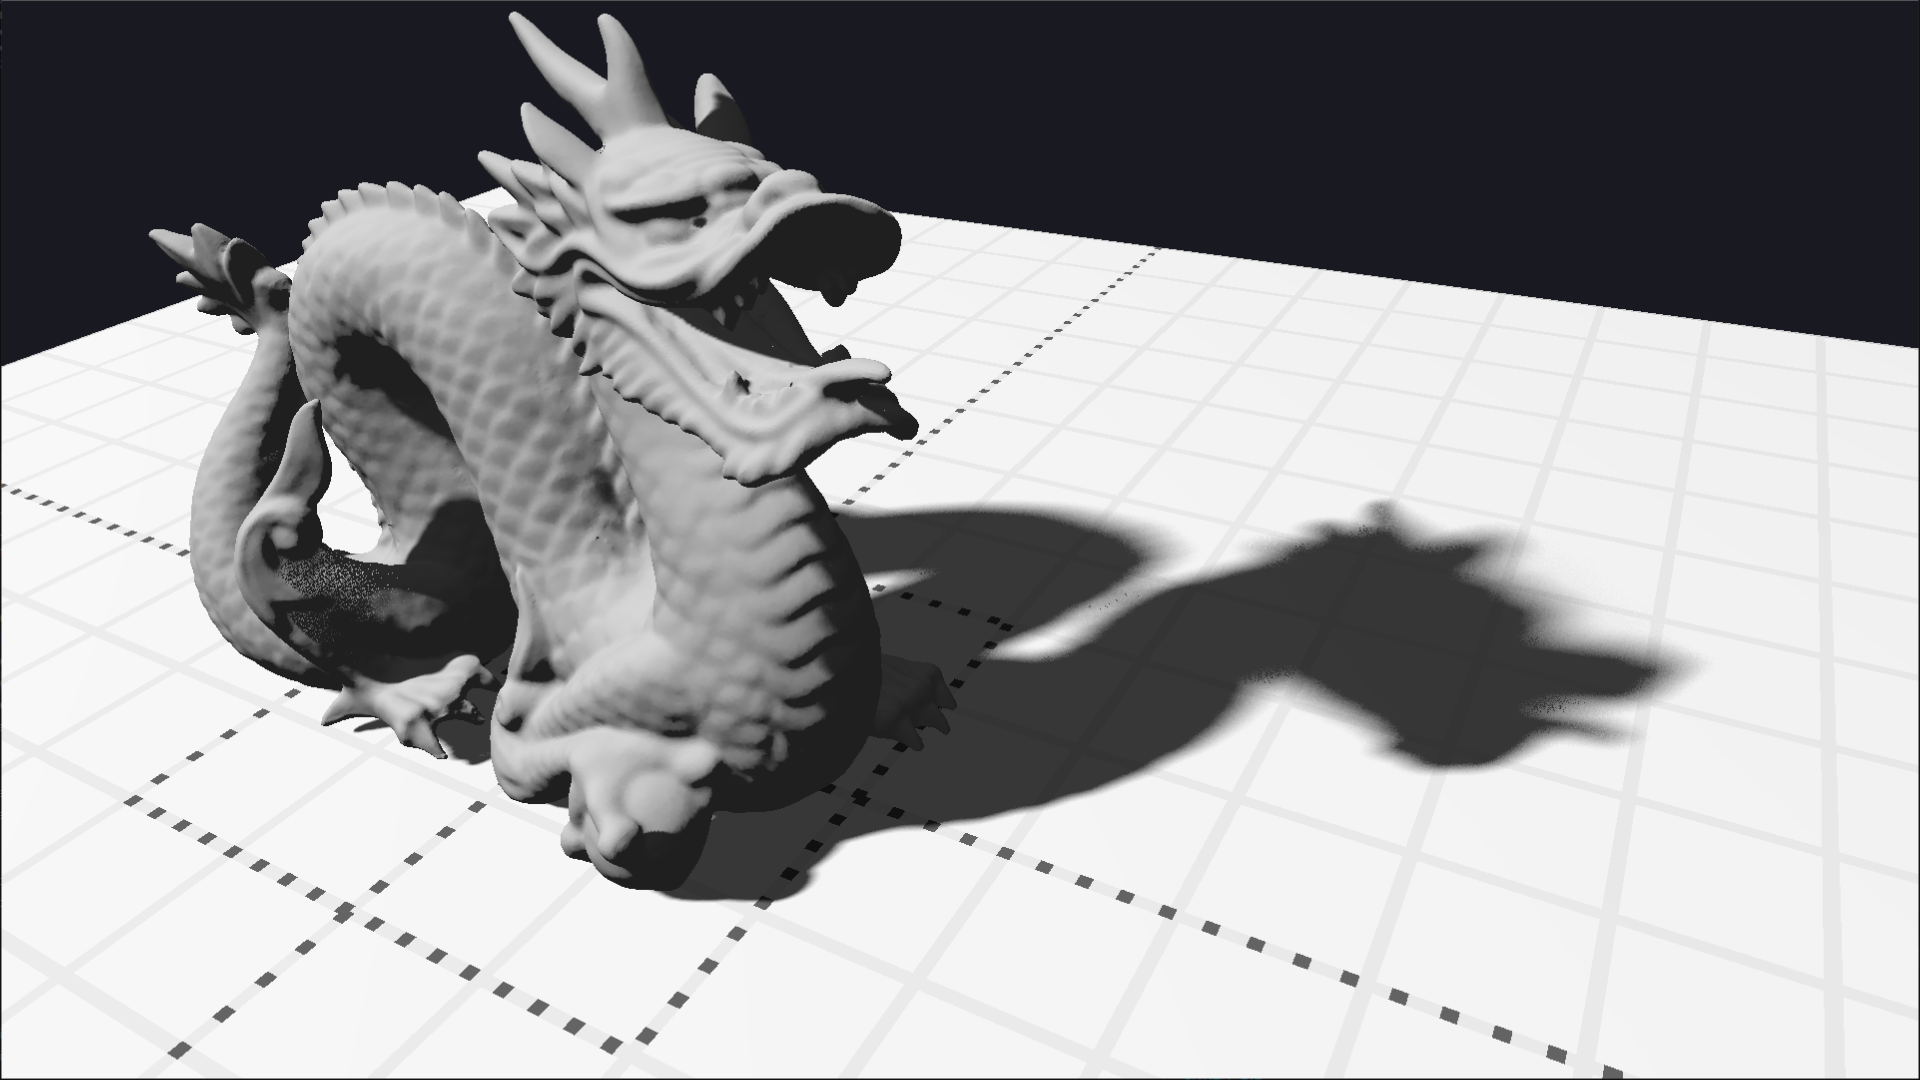
\includegraphics[width=\textwidth]{./graf/tests/pcss/cropped/dragon_pcss_1.png}
        \caption{The \textit{Chinese Dragon} showcasing contact hardening shadows.}
    \end{subfigure}
    \begin{subfigure}[t]{0.49\textwidth}
		\centering
        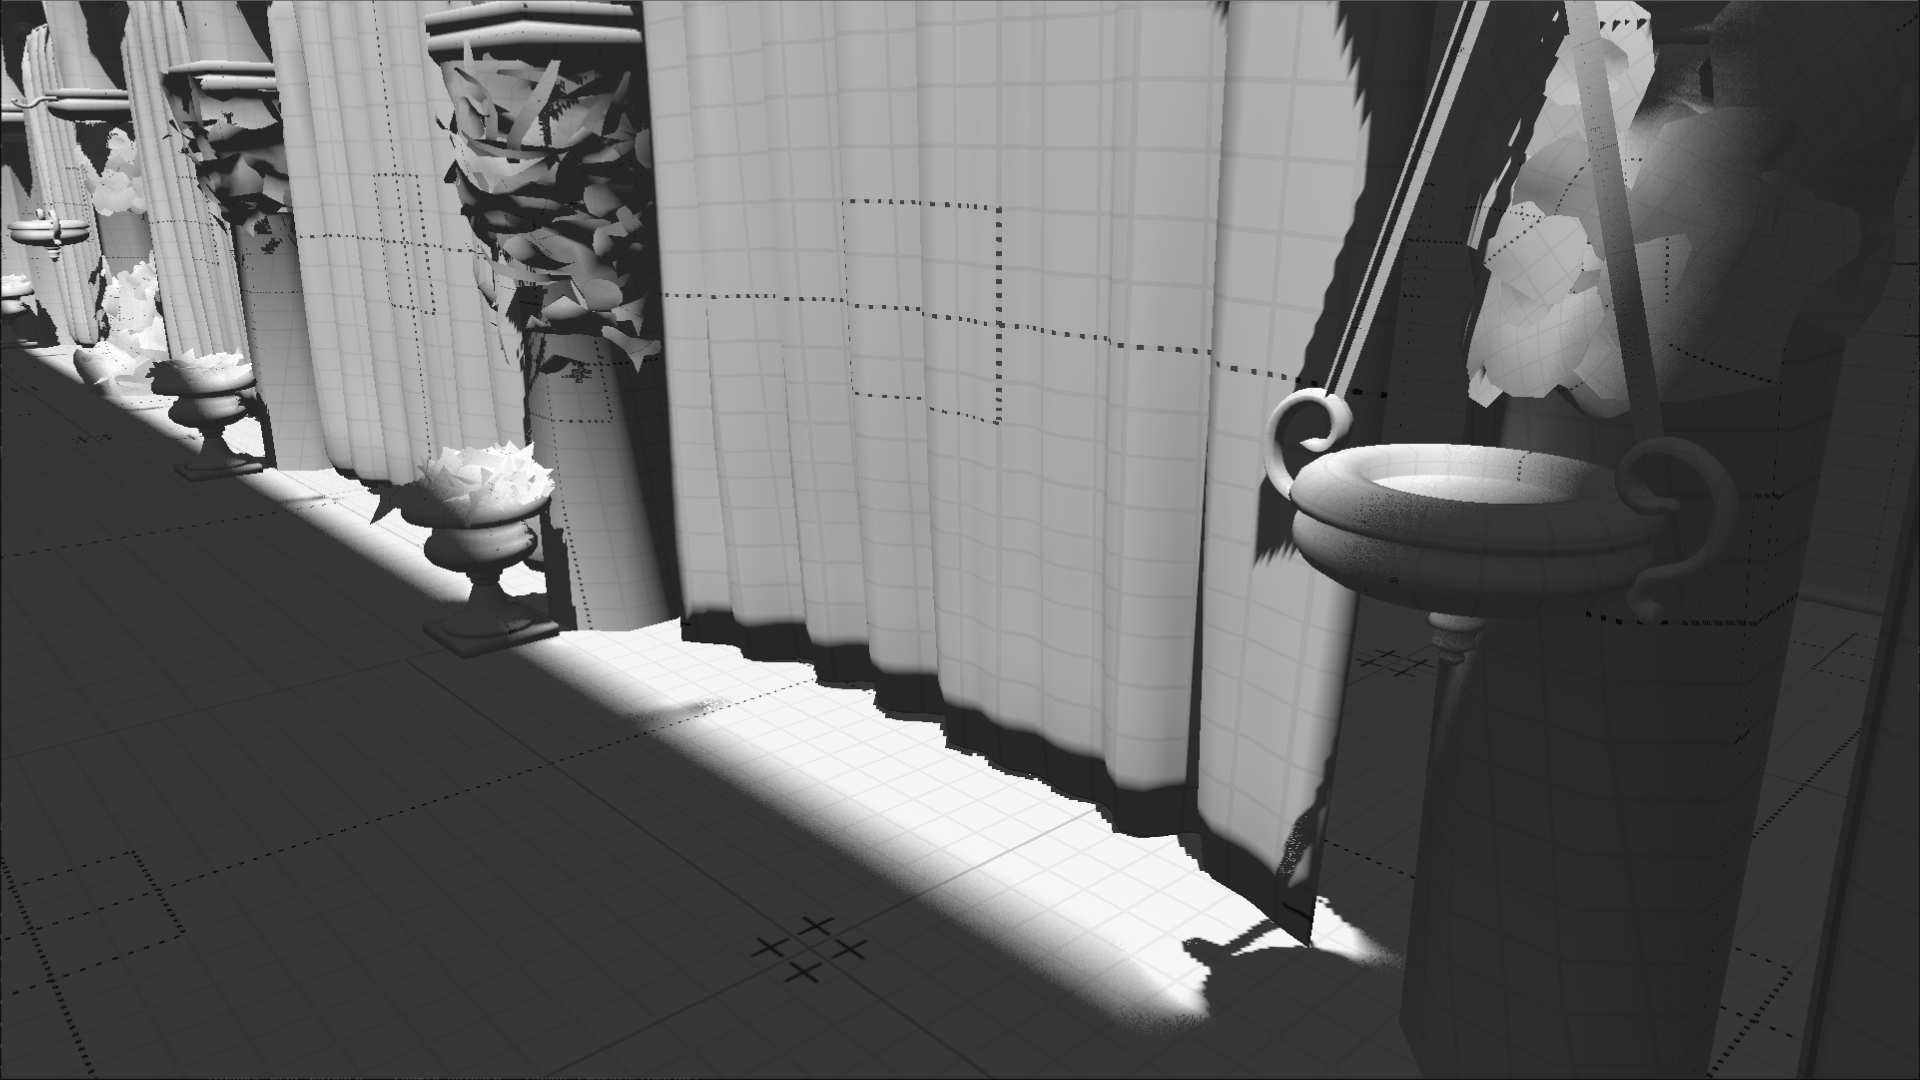
\includegraphics[width=\textwidth]{./graf/tests/pcss/cropped/sponza_pcss_1.png}
        \caption{PCSS shadows in \textit{Crytek Sponza}, creating soft shadows cast by the rooftop above and harder shadows cast by the hanging bowl.}
    \end{subfigure}
	\hfill
    \begin{subfigure}[t]{0.49\textwidth}
		\centering
        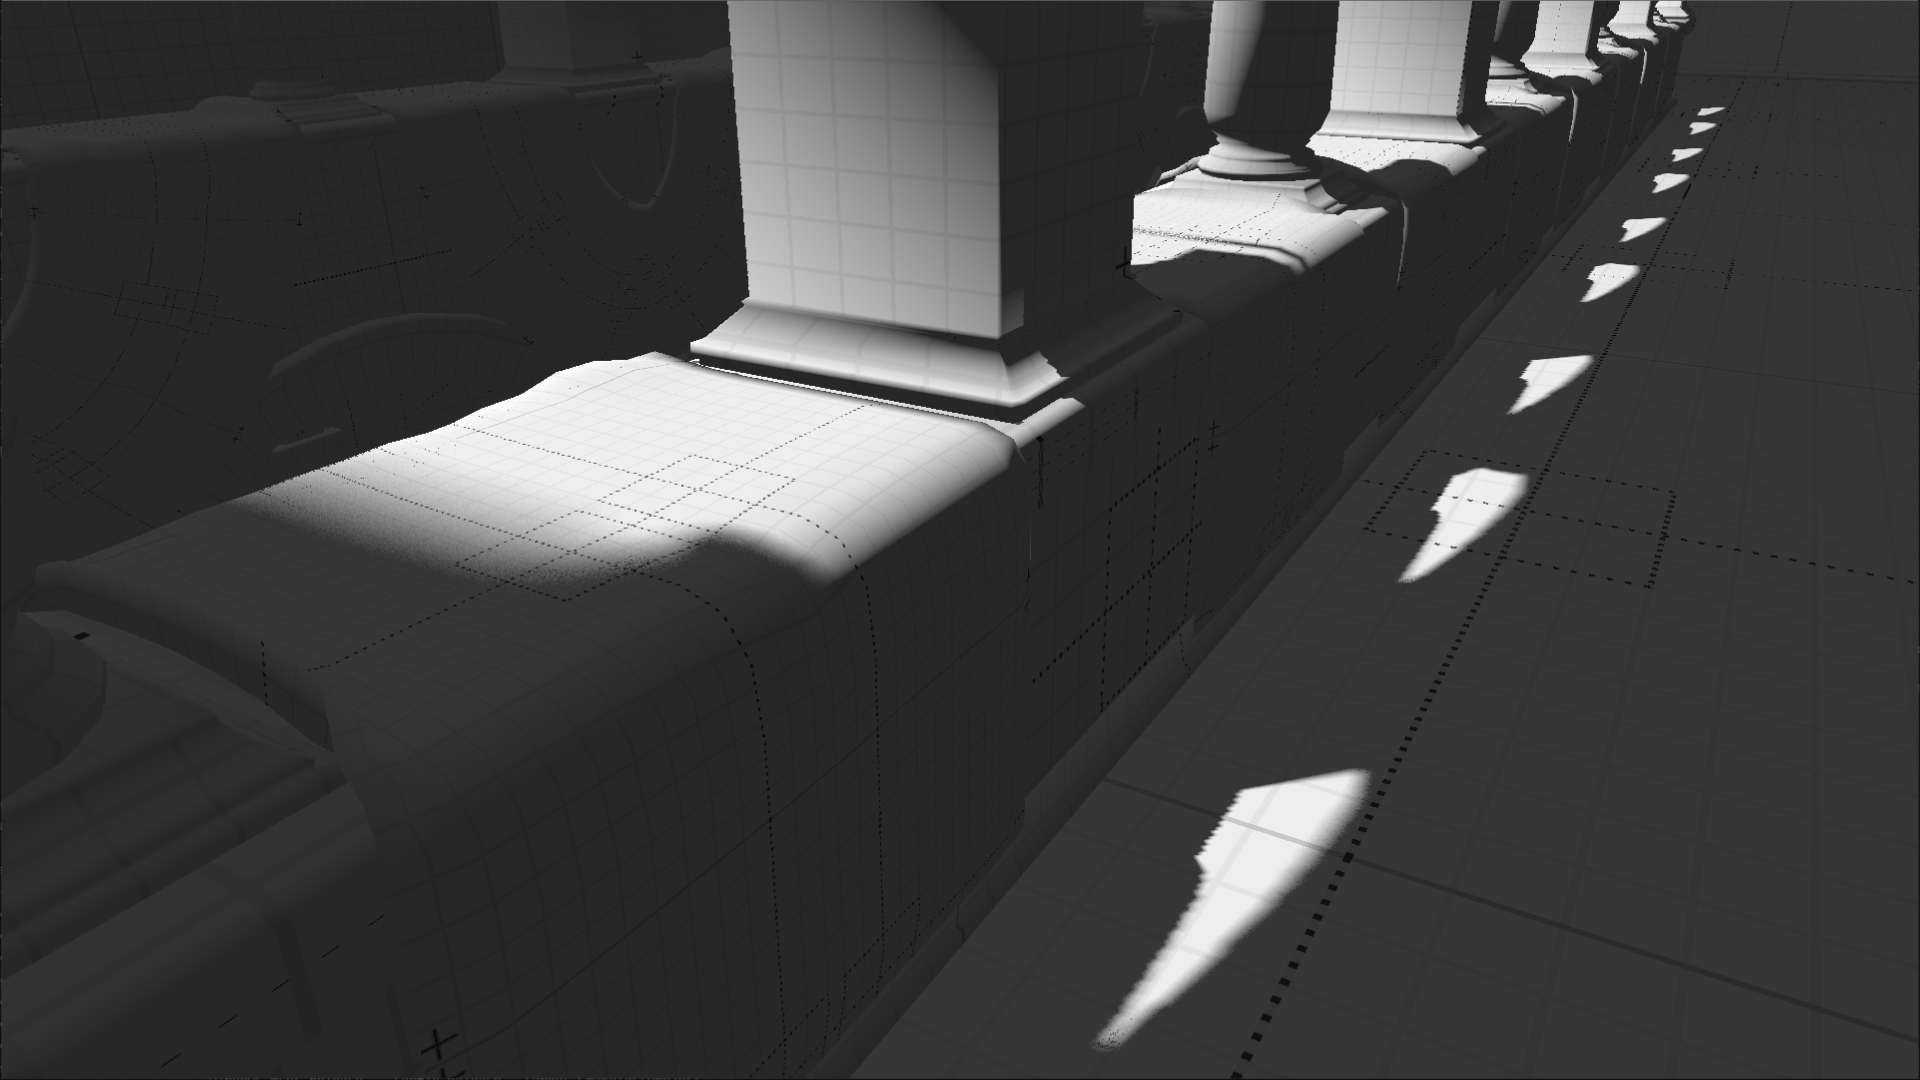
\includegraphics[width=\textwidth]{./graf/tests/pcss/cropped/sponza_pcss_2.png}
        \caption{Shadows hardening with changing distance to occluder in \textit{Crytek Sponza}.}
    \end{subfigure}

    \caption{The results of PCSS in different scenes, rendered with \(4096\times 4096\) shadow map resolution.}
    \label{fig:test_pcss_screens}
\end{figure}

PCSS has its performance cost, but the results it produces can certainly elevate the graphical presentation of a real-time application.

\section{Summary and conclusions}

Basic shadow mapping lays the foundation on which more advanced techniques can be built. It has a performance cost that is slightly smaller than double the main render pass. On its own it requires very high resolution to get pleasant results, so that aliasing it eliminated.

\begin{figure}[t]
    \centering
    \definecolor{color1}{HTML}{329BC8}
    \definecolor{color2}{HTML}{DC8952}
    \definecolor{color3}{HTML}{228E8E}
    \definecolor{color4}{HTML}{E58E98}
    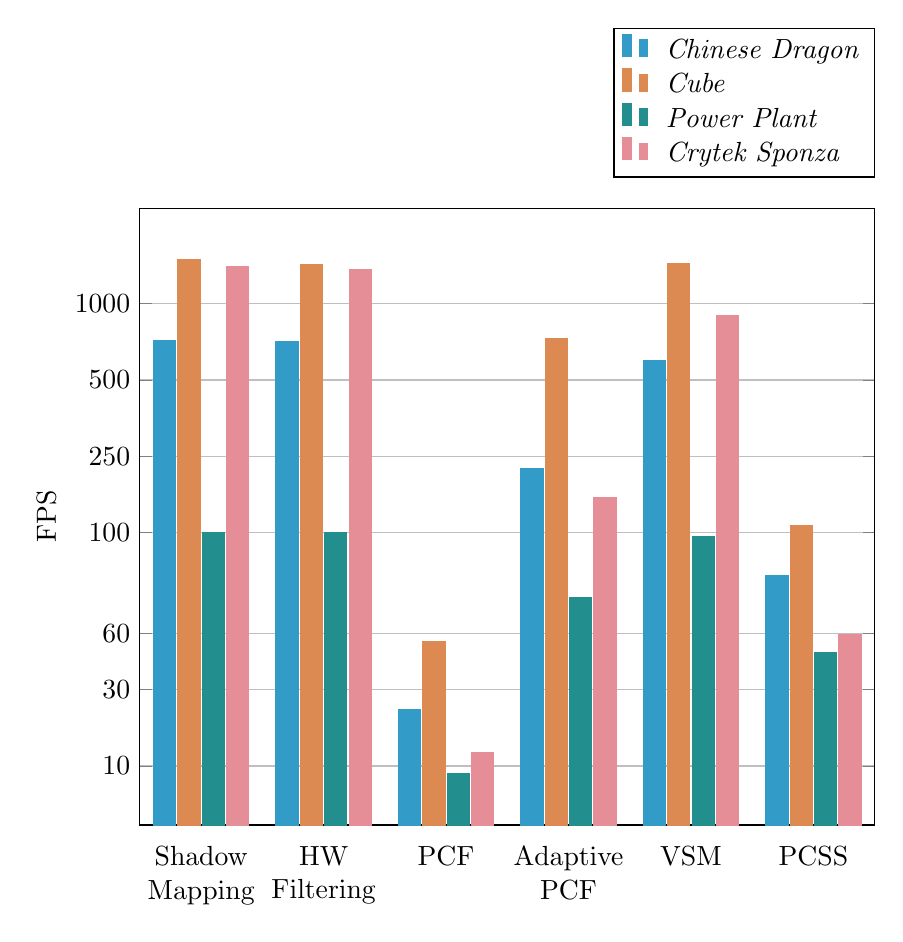
\begin{tikzpicture}
        \begin{semilogyaxis}[
            % xlabel={Shadow rendering technique},
            xlabel style = {align=center},
            ylabel={FPS},
            width  = 0.9*\textwidth,
            % height = 8cm,
            major x tick style = transparent,
            ybar=2*\pgflinewidth,
            bar width=8pt,
            ymajorgrids = true,
            ylabel = {FPS},
            ytick = {0, 10, 30, 60, 100, 250, 500, 1000, 2000},
            yticklabels = {0, 10, 30, 60, 100, 250, 500, 1000, 2000},
            x tick label style = {align=center},
            % symbolic x style = {align=center},
            symbolic x coords={Shadow\\Mapping,HW\\Filtering,PCF,Adaptive\\PCF,VSM,PCSS},
            xtick = data,
            scaled y ticks = false,
            enlarge x limits=0.1,
            % ymin=0,
            legend cell align=left,
            legend style={
                    at={(1,1.05)},
                    anchor=south east,
                    column sep=1ex
            }
        ]
            \addplot[style={color1,fill=color1,mark=none}]
                coordinates {(Shadow\\Mapping, 1428) (HW\\Filtering,1416) (PCF,50) (Adaptive\\PCF, 447) (VSM, 1192) (PCSS, 170)}; % dragon

            \addplot[style={color2,fill=color2,mark=none}]
                coordinates {(Shadow\\Mapping, 2978) (HW\\Filtering,2861) (PCF,93) (Adaptive\\PCF, 1463) (VSM, 2888) (PCSS, 267)}; % cube

            \addplot[style={color3,fill=color3,mark=none}]
                coordinates {(Shadow\\Mapping, 251) (HW\\Filtering,250) (PCF,28) (Adaptive\\PCF, 138) (VSM, 241) (PCSS, 84)}; % power

            \addplot[style={color4,fill=color4,mark=none}]
                coordinates {(Shadow\\Mapping, 2795) (HW\\Filtering,2736) (PCF,34) (Adaptive\\PCF, 343) (VSM, 1800) (PCSS, 99)}; % sponza

            \legend{\textit{Chinese Dragon},\textit{Cube},\textit{Power Plant},\textit{Crytek Sponza}}
        \end{semilogyaxis}
    \end{tikzpicture}
    \caption{Average measured frame rates for all test scenes and all tested techniques, at \(1024\times 1024\) shadow map resolution, \(1920\times 1080\) screen resolution, \(11\times 11\) filter kernel size (for PCF, adaptive PCF, PCSS and VSM). For PCSS light source size of 0.4 was assumed.}
    \label{fig:plot:summary_fps}
\end{figure}

It can be enhanced with various filtering methods. Bilinear comparison filtering is implemented within GPU hardware, so it can be very fast. It can be used to blur the edges of shadows for almost no performance cost. This helps separate hard shadows from actual geometry. Percentage-closer filtering allows control over the strength and quality of the shadow smoothing effect. It uses a square filter kernel to average shadow function results. The performance drops very rapidly with increase in the filer size and the results feature quite severe banding and visible shadow map texel borders. This can be greatly improved by combining PCF with hardware bilinear filtering. Then, even a very small shadow map and a modestly sized kernel can produce very pleasant shadows. Adaptive PCF improves both performance and visual results. By using sets of filter kernels stored in a 3D texture, the algorithm can quit filtering early where further samples are not required. The blurring gives very smooth results, hiding any banding or texel boundaries and is easily controllable. Adaptive PCF increases the memory consumption by \(m\times m\times (n^2 / 2)\). It can also unfortunately introduce high-contrast noise in specific areas of the shadows. VSM offers outstanding performance by enabling the use of typical texture filtering operations and separable manual filtering. It does not suffer from shadow acne, but has its own issues with light leaks. It produces very pleasant shadows that exhibit certain softness, but at the same time they can lack in detail. Additionally, VSM requires up to five times more memory than regular shadow mapping.

Finally, percentage-closer soft shadows can be used to render contact-hardening shadows. This technique gives the most robust visuals, but requires careful hand tuning of the parameters such as bias and light size. It gives realistic looking results, which are however not physically correct, and are only an approximation. The performance cost is approximately twice that of adaptive PCF on its own.

Figure \ref{fig:plot:summary_fps} presents aggregated frame rate results for all tested algorithms for \(1024\times 1024\) shadow maps, filter kernel size \(11\times 11\) (where applicable) and output resolution of \(1920\times 1080\).

If the visuals are of the highest importance and the application has a lot of frame time budget available, PCSS is the best choice. VSM is both very performant and gives very smooth shadows, but should be reconsidered if shadow detail is important. In other cases, a balance between shadow map resolution, kernel size and kernel offset scale should be found within adaptive PCF. Basic PCF should probably be avoided, unless combining a small kernel size with hardware bilinear filtering and high shadow map resolution for basic anti-aliasing of shadows. Table \ref{fig:table:breakdown} contains a summary of visual aspects of the techniques.

\begin{table}[h]
    \centering
    \caption{Breakdown of visual characteristics of all tested techniques. `$\sim$' means partially applicable.}
    \label{fig:table:breakdown}
    \begin{tabular}{|>{\columncolor[HTML]{EFEFEF}}l |l|l|l|l|l|l|}
    \hline
    \cellcolor[HTML]{D0D0D0}{\color[HTML]{000000} Characteristics} &
      \multicolumn{1}{c|}{\cellcolor[HTML]{EFEFEF}{\color[HTML]{000000} \textbf{\begin{tabular}[c]{@{}c@{}}Shadow\\ mapping\end{tabular}}}} &
      \multicolumn{1}{c|}{\cellcolor[HTML]{EFEFEF}{\color[HTML]{000000} \textbf{\begin{tabular}[c]{@{}c@{}}HW\\ Filtering\end{tabular}}}} &
      \multicolumn{1}{c|}{\cellcolor[HTML]{EFEFEF}{\color[HTML]{000000} \textbf{PCF}}} &
      \multicolumn{1}{c|}{\cellcolor[HTML]{EFEFEF}{\color[HTML]{000000} \textbf{\begin{tabular}[c]{@{}c@{}}Adaptive\\ PCF\end{tabular}}}} &
      \multicolumn{1}{c|}{\cellcolor[HTML]{EFEFEF}{\color[HTML]{000000} \textbf{VSM}}} &
      \multicolumn{1}{c|}{\cellcolor[HTML]{EFEFEF}{\color[HTML]{000000} \textbf{PCSS}}} \\ \hline
    {\color[HTML]{000000} \textbf{\begin{tabular}[c]{@{}l@{}}Precise\\ shadows\end{tabular}}} &
      {\color[HTML]{000000} Yes} &
      {\color[HTML]{000000} Yes} &
      {\color[HTML]{000000} Yes} &
      {\color[HTML]{000000} Yes} &
      {\color[HTML]{000000} $\sim$} &
      {\color[HTML]{000000} Yes} \\ \hline
    {\color[HTML]{000000} \textbf{Soft shadows}} &
      {\color[HTML]{000000} No} &
      {\color[HTML]{000000} No} &
      {\color[HTML]{000000} Yes} &
      {\color[HTML]{000000} Yes} &
      {\color[HTML]{000000} Yes} &
      {\color[HTML]{000000} Yes} \\ \hline
    {\color[HTML]{000000} \textbf{Anti-aliasing}} &
      {\color[HTML]{000000} No} &
      {\color[HTML]{000000} $\sim$} &
      {\color[HTML]{000000} $\sim$} &
      {\color[HTML]{000000} Yes} &
      {\color[HTML]{000000} Yes} &
      {\color[HTML]{000000} Yes} \\ \hline
    {\color[HTML]{000000} \textbf{\begin{tabular}[c]{@{}l@{}}Contact-hardening\\ shadows\end{tabular}}} &
      {\color[HTML]{000000} No} &
      {\color[HTML]{000000} No} &
      {\color[HTML]{000000} No} &
      {\color[HTML]{000000} No} &
      {\color[HTML]{000000} No} &
      {\color[HTML]{000000} Yes} \\ \hline
    {\color[HTML]{000000} \textbf{Surface acne-free}} &
      {\color[HTML]{000000} No} &
      {\color[HTML]{000000} No} &
      {\color[HTML]{000000} No} &
      {\color[HTML]{000000} No} &
      {\color[HTML]{000000} Yes} &
      {\color[HTML]{000000} No} \\ \hline
    {\color[HTML]{000000} \textbf{Noise-free}} &
      {\color[HTML]{000000} Yes} &
      {\color[HTML]{000000} Yes} &
      {\color[HTML]{000000} Yes} &
      {\color[HTML]{000000} No} &
      {\color[HTML]{000000} No} &
      {\color[HTML]{000000} No} \\ \hline
    \end{tabular}
\end{table}

% \begin{table}
% \centering
% \caption{A caption of a table is ABOVE it.}
% \label{id:tab:wyniki}
% \begin{tabular}{rrrrrrrr}
% \toprule
% 	         &                                     \multicolumn{7}{c}{method}                                      \\
% 	         \cmidrule{2-8}
% 	         &         &         &        \multicolumn{3}{c}{alg. 3}        & \multicolumn{2}{c}{alg. 4, $\gamma = 2$} \\
% 	         \cmidrule(r){4-6}\cmidrule(r){7-8}
% 	$\zeta$ &     alg. 1 &   alg. 2 & $\alpha= 1.5$ & $\alpha= 2$ & $\alpha= 3$ &   $\beta = 0.1$  &   $\beta = -0.1$ \\
% \midrule
% 	       0 &  8.3250 & 1.45305 &       7.5791 &    14.8517 &    20.0028 & 1.16396 &                       1.1365 \\
% 	       5 &  0.6111 & 2.27126 &       6.9952 &    13.8560 &    18.6064 & 1.18659 &                       1.1630 \\
% 	      10 & 11.6126 & 2.69218 &       6.2520 &    12.5202 &    16.8278 & 1.23180 &                       1.2045 \\
% 	      15 &  0.5665 & 2.95046 &       5.7753 &    11.4588 &    15.4837 & 1.25131 &                       1.2614 \\
% 	      20 & 15.8728 & 3.07225 &       5.3071 &    10.3935 &    13.8738 & 1.25307 &                       1.2217 \\
% 	      25 &  0.9791 & 3.19034 &       5.4575 &     9.9533 &    13.0721 & 1.27104 &                       1.2640 \\
% 	      30 &  2.0228 & 3.27474 &       5.7461 &     9.7164 &    12.2637 & 1.33404 &                       1.3209 \\
% 	      35 & 13.4210 & 3.36086 &       6.6735 &    10.0442 &    12.0270 & 1.35385 &                       1.3059 \\
% 	      40 & 13.2226 & 3.36420 &       7.7248 &    10.4495 &    12.0379 & 1.34919 &                       1.2768 \\
% 	      45 & 12.8445 & 3.47436 &       8.5539 &    10.8552 &    12.2773 & 1.42303 &                       1.4362 \\
% 	      50 & 12.9245 & 3.58228 &       9.2702 &    11.2183 &    12.3990 & 1.40922 &                       1.3724 \\
% \bottomrule
% \end{tabular}
% \end{table}  

% The table is here too \ref{id:tab:wyniki}

%%%%%%%%%%%%%%%%%%%%%
% FIGURE FROM FILE
%
% \begin{figure}
% \centering
% 
\includegraphics[width=0.5\textwidth]{./graf/politechnika_sl_logo_bw_pion_en.pdf}
% \caption{Caption of a figure is always below the figure.}
% \label{fig:label}
% \end{figure}

% Fig. \ref{fig:label} presents asdasd

% \begin{figure}
% 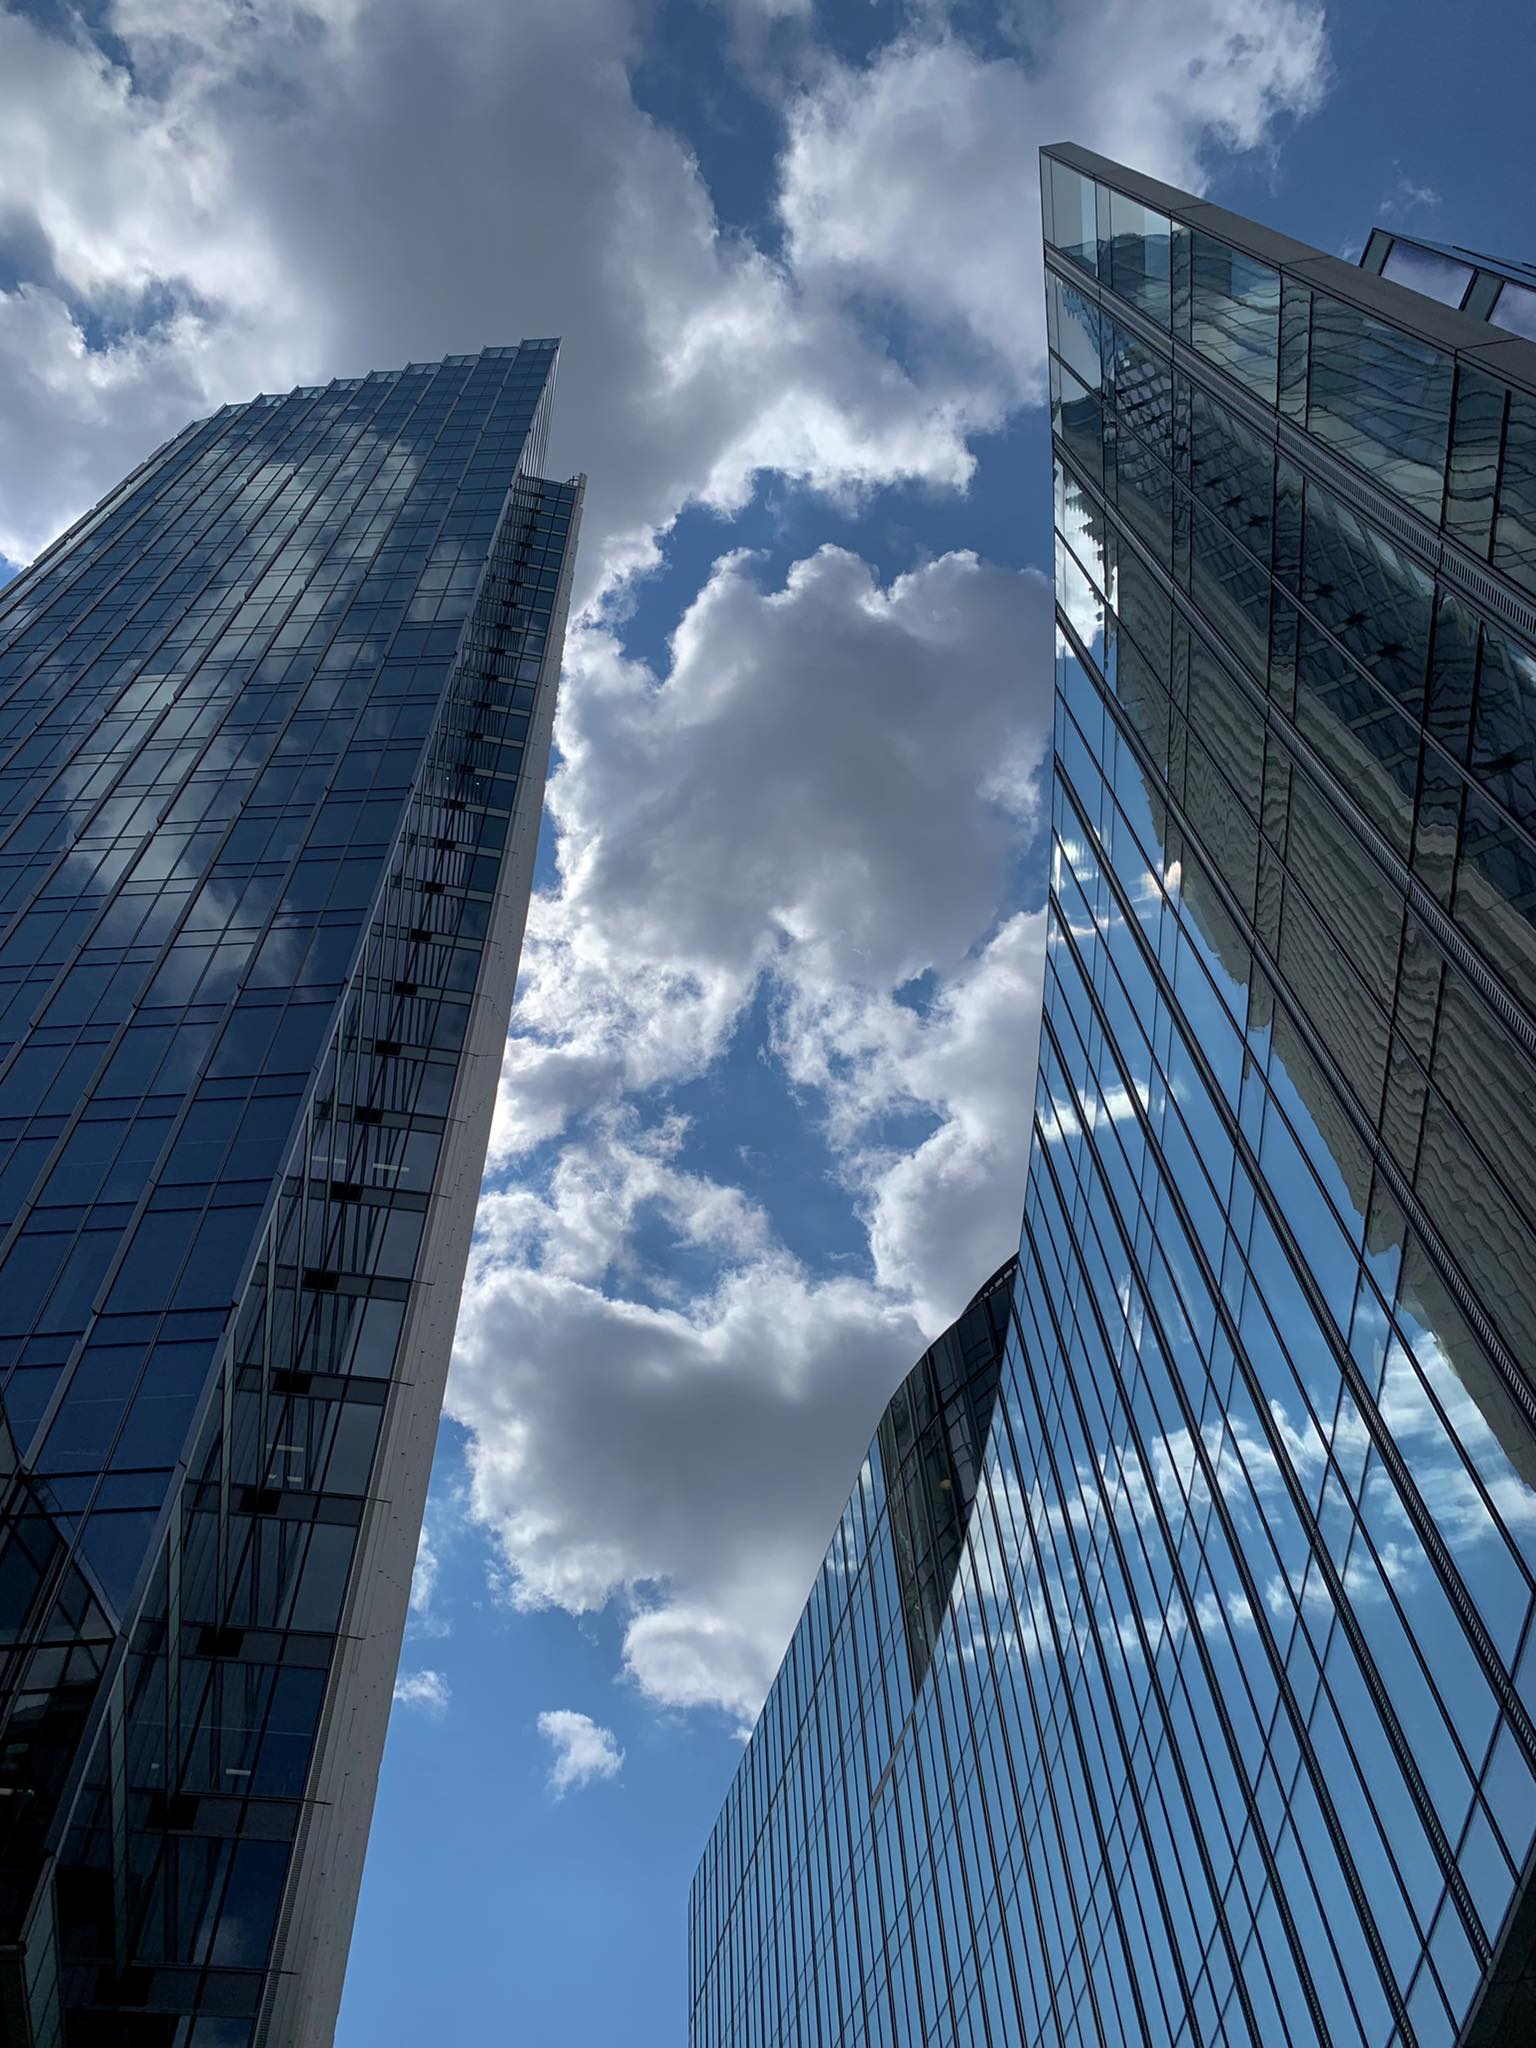
\includegraphics[width=0.5\textwidth]{./graf/test_image.jpg}
% \caption{Caption of a figure is always below the figure akakak.}
% \label{fig:duped_image3}
% \end{figure}

% some citation of the above \ref{fig:duped_image3}

%%%%%%%%%%%%%%%%%%%%%
%
%%%%%%%%%%%%%%%%%%%%
%% SUBFIGURES
%
% \begin{figure}
% \centering
% \begin{subfigure}{0.4\textwidth}
%    
\includegraphics[width=\textwidth]{./graf/politechnika_sl_logo_bw_pion_en.pdf}
%    \caption{Upper left figure.}
%    \label{fig:upper-left}
% \end{subfigure}
% \hfill
% \begin{subfigure}{0.4\textwidth}
%    
\includegraphics[width=\textwidth]{./graf/politechnika_sl_logo_bw_pion_en.pdf}
%    \caption{Upper right figure.}
%    \label{fig:upper-right}
% \end{subfigure}

% \begin{subfigure}{0.4\textwidth}
%    
\includegraphics[width=\textwidth]{./graf/politechnika_sl_logo_bw_pion_en.pdf}
%    \caption{Lower left figure.}
%    \label{fig:lower-left}
% \end{subfigure}
% \hfill
% \begin{subfigure}{0.4\textwidth}
%    
\includegraphics[width=\textwidth]{./graf/politechnika_sl_logo_bw_pion_en.pdf}
%    \caption{Lower right figure.}
%    \label{fig:lower-right}
% \end{subfigure}
       
% \caption{Common caption for all subfigures.}
% \label{fig:subfigures}
% \end{figure}
% Fig. \ref{fig:subfigures} presents very important information, eg. Fig. \ref{fig:upper-right} is an upper right subfigure.
%%%%%%%%%%%%%%%%%%%%%



% \begin{figure}
% \centering
% \begin{tikzpicture}
% \begin{axis}[
%    y tick label style={
%        /pgf/number format/.cd,
%            fixed,   % po zakomentowaniu os rzednych jest indeksowana wykladniczo
%            fixed zerofill, % 1.0 zamiast 1
%            precision=1,
%        /tikz/.cd
%    },
%    x tick label style={
%        /pgf/number format/.cd,
%            fixed,
%            fixed zerofill,
%            precision=2,
%        /tikz/.cd
%    }
% ]
% \addplot [domain=0.0:0.1] {rnd};
% \end{axis} 
% \end{tikzpicture}
% \caption{Figure caption is BELOW the figure.}
% \label{fig:3}
% \end{figure}

% \begin{figure}
% \centering
% 
\includegraphics[width=0.5\textwidth]{./graf/politechnika_sl_logo_bw_pion_en.pdf}
% \caption{Caption of a figure is always below the figure akakak.}
% \label{fig:3}
% \end{figure}

% some citation of the above \ref{fig:3}

% \begin{figure}
% \begin{lstlisting}
% if (_nClusters < 1)
% 	throw std::string ("unknown number of clusters");
% if (_nIterations < 1 and _epsilon < 0)
% 	throw std::string ("You should set a maximal number of iteration or minimal difference -- epsilon.");
% if (_nIterations > 0 and _epsilon > 0)
% 	throw std::string ("Both number of iterations and minimal epsilon set -- you should set either number of iterations or minimal epsilon.");
% \end{lstlisting}
% \caption{Example of pseudocode.}
% \end{figure}